\documentclass[journal,compsoc,10pt]{IEEEtran}
\usepackage[utf8]{inputenc}
\usepackage[T1]{fontenc}
\usepackage{mathptmx}
\usepackage[scaled=.90]{helvet}
\usepackage{courier}
\usepackage{microtype}
\usepackage[hyphens]{url}
\usepackage{cite}
\usepackage{amsmath,amssymb,amsfonts,amsthm,mathtools}
\usepackage{graphicx}
\usepackage{xcolor}
\usepackage{booktabs}
\usepackage{makecell}
\usepackage{multirow}
\usepackage{enumitem}
\usepackage{tikz}
\usetikzlibrary{positioning,arrows.meta,calc,decorations.pathreplacing}
\usepackage{pgfplots}
\pgfplotsset{compat=1.17}
\usepackage[colorlinks=true,linkcolor=black,citecolor=black,urlcolor=black]{hyperref}
\usepackage[noabbrev,capitalize]{cleveref}
\sloppy
\emergencystretch=2em
\hbadness=3000

% ---- theorem environments ----
\theoremstyle{definition}
\newtheorem{definition}{Definition}
\theoremstyle{plain}
\newtheorem{theorem}{Theorem}
\newtheorem{lemma}{Lemma}
\newtheorem{proposition}{Proposition}
\theoremstyle{remark}
\newtheorem*{observation}{Observation}
\crefname{definition}{Definition}{Definitions}
\Crefname{definition}{Definition}{Definitions}
\Crefname{proposition}{Proposition}{Propositions}

% ---- field macros (as in the artifact) ----
\newcommand{\fld}[1]{\mathit{#1}}
\newcommand{\rs}{\fld{read\_set}}
\newcommand{\ws}{\fld{write\_set}}
\newcommand{\rt}{\fld{read\_time}}
\newcommand{\wt}{\fld{write\_time}}
\newcommand{\rv}{\fld{read\_values}}
\newcommand{\wv}{\fld{write\_values}}
\newcommand{\rreg}{\fld{read\_registry}}
\newcommand{\wreg}{\fld{write\_registry}}
\newcommand{\pt}{\fld{planned\_tool}}
\newcommand{\tool}[1]{\texttt{#1}}
\newcommand{\A}[1]{$A_{#1}$}
\newcommand{\Rp}{$R$}                      % the residue predicate (artifact name: NoA7 / SupersededBasisEffect)
\newcommand{\Lv}[1]{$L_{#1}$}
\newcommand{\TLA}{TLA\textsuperscript{+}}
\newcommand{\ie}{i.e.}
\newcommand{\eg}{e.g.}

% ---- numbers that the experiment kit regenerates (one place to edit) ----
% ============================================================================
% claims.tex: every headline number (one definition each; comments give the receipt)
% ============================================================================
% claims.tex -- every headline number, as a macro.  Regenerate with
%   python3 harness/macaudit/claims_to_tex.py CLAIMS.json > paper/claims.tex
% so that the paper and CLAIMS.json cannot drift.  VERIFIED-HERE = re-derived
% from committed receipts in this audit; PAPER = carried from the submitted
% artifact's receipts and gated by reproduce.sh but not re-run in this audit.

% --- formal (VERIFIED-HERE unless noted) ---
\newcommand{\VerusCurated}{371}        % PAPER: verus_count.sh under the pinned build 0.2026.09.13 (364 + the 7 of lib_l5_ledger.rs), 2026-10-13
\newcommand{\VerusFull}{392}           % PAPER: verus_count.sh --full under the pinned build
\newcommand{\VerusLoadBearing}{236}    % arithmetic on the per-file table (Sec. 5)
\newcommand{\VerusScaffold}{135}       % arithmetic on the per-file table (+7: the ledger file)
\newcommand{\VerusDetector}{24}        % PAPER
\newcommand{\TlapsHierarchy}{15}       % log committed
\newcommand{\TlapsLowerBound}{28}      % log committed
\newcommand{\TlapsCommitOrder}{60}     % PAPER; tlapm log committed 2026-10-14: formal/tla/tlaps.CommitOrder.log ("All 60 obligations proved")
\newcommand{\CommitOrderVerdicts}{15}  % VERIFIED-HERE
\newcommand{\CommitOrderHistories}{35{,}659}      % VERIFIED-HERE
\newcommand{\CommitOrderMemoryStates}{2{,}961{,}434} % VERIFIED-HERE
\newcommand{\LatticeRuns}{64}          % VERIFIED-HERE (6-run sample identical to reference; full matrix in reference json)
\newcommand{\LatticeMaxOpsThreeRuns}{16}
\newcommand{\LatticeSafeStatesMin}{380{,}920}
\newcommand{\LatticeSafeStatesMax}{2{,}015{,}279}

% --- live LangGraph A1 study (VERIFIED-HERE, incl. the outcome columns) ---
\newcommand{\LiveNPerCell}{100}
\newcommand{\LiveGptVanillaAOne}{60}
\newcommand{\LiveHaikuVanillaAOne}{91}
\newcommand{\LiveLlamaVanillaAOne}{1}
\newcommand{\LiveGptValidatedWrong}{34}
\newcommand{\LiveHaikuValidatedWrong}{7}
\newcommand{\LiveLlamaValidatedWrong}{100}
\newcommand{\LiveGptRegen}{66}
\newcommand{\LiveHaikuRegen}{93}
\newcommand{\LiveGptPinnedMean}{1.07}
\newcommand{\LiveGptPinnedMax}{3.79}
\newcommand{\LiveHaikuPinnedMean}{1.21}
\newcommand{\LiveHaikuPinnedMax}{1.96}
\newcommand{\LiveLlamaPinnedMean}{3.77}
\newcommand{\LiveLlamaPinnedMax}{9.06}
\newcommand{\LiveOffsetMs}{150}
\newcommand{\SuperstepGpt}{42}
\newcommand{\SuperstepHaiku}{72}
\newcommand{\SuperstepLlama}{26}

% --- AutoGen pilot (VERIFIED-HERE via rescore) ---
\newcommand{\PilotTriageRates}{42\%, 48\% and 52\%}
\newcommand{\PilotTriagePooled}{142/300}
\newcommand{\PilotSiEditResidual}{5}
\newcommand{\PilotSiTriageResidual}{8}

% --- cost (VERIFIED-HERE: workcost.py, realstore_metrics.py --check) ---
\newcommand{\CostRun}{20260913T0150Z}

% --- L2 / L4 / A6 (PAPER; receipts to be committed as results/*.json) ---
\newcommand{\LtwoDefThreeBaseline}{519, 624 and 563}
\newcommand{\LtwoExposedBaseline}{1{,}538, 2{,}059 and 2{,}010}
\newcommand{\LtwoExposedVerified}{402, 547 and 549}
\newcommand{\LtwoRelabeled}{767, 1{,}288 and 1{,}239}
\newcommand{\LiveLtwoRetractions}{66}
\newcommand{\LfourPhantom}{630, 505 and 387}

% --- ToolNode A6 (VERIFIED-HERE from per-turn receipts) ---
\newcommand{\ToolNodeGptBatched}{30}
\newcommand{\ToolNodeGptReordered}{22}
\newcommand{\ToolNodeGptFull}{18}
\newcommand{\ToolNodeLlamaBatched}{3}
\newcommand{\ToolNodeLlamaReordered}{2}
\newcommand{\ToolNodeBatchedTurns}{33}
\newcommand{\ToolNodeReorderings}{24}

% --- census (VERIFIED-HERE: langgraph_census.py --summary/--check) ---
\newcommand{\CensusRepos}{98}
\newcommand{\CensusSites}{407}
\newcommand{\CensusSequential}{392}
\newcommand{\CensusParallelRepos}{11}
\newcommand{\CensusUpperRepos}{8}
\newcommand{\CensusErrorStringRepos}{34}

% --- residue predicate R (artifact: A7 / NoA7) and the ledger (added 2026-10-13) ---
% VERIFIED-HERE: A7 witness (3 s), NoA7 exhaustive under G7 (5,213,012 states; 9,688,601 with G3), the full lattice32 matrix (160 runs, 0 mismatches),
% the partition A1+A7 = booking!=final on every live cell (harness/macaudit/a7_rescore.py --check).
\newcommand{\AsevenGptVanilla}{40}
\newcommand{\AsevenHaikuVanilla}{9}
\newcommand{\AsevenLlamaVanilla}{99}
\newcommand{\AsevenGptValidated}{34}
\newcommand{\AsevenHaikuValidated}{7}
\newcommand{\AsevenLlamaValidated}{100}
\newcommand{\LatticeThirtyTwoRuns}{160}
\newcommand{\LatticeThirtyTwoSafeMin}{1{,}803{,}848}   % VERIFIED-HERE (lattice32_results.reference.json)
\newcommand{\LatticeThirtyTwoSafeMax}{9{,}688{,}601}
\newcommand{\NoAsevenStates}{5{,}213{,}012}
\newcommand{\NoAsevenStatesGthree}{9{,}688{,}601}
% PENDING (your machine): verus count for lib_l5_ledger.rs; probe 303 --modes ledger outcome
\newcommand{\LfiveVerus}{7 obligations, 0 errors}   % results/verus/lib_l5_ledger.verus.log, pinned build
% short forms for the abstract / intro: replace with "verified, N obligations" once lib_l5_ledger.rs verifies
\newcommand{\LfiveVerusStatus}{verified in Verus (7 obligations, 0 errors)}
\newcommand{\LfiveVerusIntro}{verified (7 obligations)}
\newcommand{\LfiveLiveOutcome}{\textbf{[probe 303 -{}-modes ledger: pending]}}
% per-cell defaults for the verified / ledger rows of Table 3 ("--" = pending); claims_results.tex overrides
\newcommand{\Pend}{--}
\newcommand{\LiveVerifiedGptAOne}{\Pend}\newcommand{\LiveVerifiedGptR}{\Pend}\newcommand{\LiveVerifiedGptWrong}{\Pend}\newcommand{\LiveVerifiedGptRegen}{\Pend}
\newcommand{\LiveVerifiedHaikuAOne}{\Pend}\newcommand{\LiveVerifiedHaikuR}{\Pend}\newcommand{\LiveVerifiedHaikuWrong}{\Pend}\newcommand{\LiveVerifiedHaikuRegen}{\Pend}
\newcommand{\LiveLedgerGptAOne}{\Pend}\newcommand{\LiveLedgerGptR}{\Pend}\newcommand{\LiveLedgerGptWrong}{\Pend}\newcommand{\LiveLedgerGptRegen}{\Pend}
\newcommand{\LiveLedgerHaikuAOne}{\Pend}\newcommand{\LiveLedgerHaikuR}{\Pend}\newcommand{\LiveLedgerHaikuWrong}{\Pend}\newcommand{\LiveLedgerHaikuRegen}{\Pend}
\newcommand{\LiveVerifiedLlamaAOne}{\Pend}\newcommand{\LiveVerifiedLlamaR}{\Pend}\newcommand{\LiveVerifiedLlamaWrong}{\Pend}\newcommand{\LiveVerifiedLlamaRegen}{\Pend}
\newcommand{\LiveLedgerLlamaAOne}{\Pend}\newcommand{\LiveLedgerLlamaR}{\Pend}\newcommand{\LiveLedgerLlamaWrong}{\Pend}\newcommand{\LiveLedgerLlamaRegen}{\Pend}
% probe 301 / 302 defaults
\newcommand{\ToolNodeRealSqlite}{\textbf{[probe 301: pending]}}
\newcommand{\ToolNodeRealHttp}{\textbf{[probe 301: pending]}}
\newcommand{\WallclockPairedGptAvailable}{0}\newcommand{\WallclockPairedClaudeAvailable}{0}
\newcommand{\WallclockPairedGptTriagePess}{\Pend}\newcommand{\WallclockPairedGptTriageSI}{\Pend}
\newcommand{\WallclockPairedGptEditReviewPess}{\Pend}\newcommand{\WallclockPairedGptEditReviewSI}{\Pend}
\newcommand{\WallclockPairedGptPlanExecutePess}{\Pend}\newcommand{\WallclockPairedGptPlanExecuteSI}{\Pend}
\newcommand{\WallclockPairedClaudeTriagePess}{\Pend}\newcommand{\WallclockPairedClaudeTriageSI}{\Pend}
\newcommand{\WallclockPairedClaudeEditReviewPess}{\Pend}\newcommand{\WallclockPairedClaudeEditReviewSI}{\Pend}
\newcommand{\WallclockPairedClaudePlanExecutePess}{\Pend}\newcommand{\WallclockPairedClaudePlanExecuteSI}{\Pend}
\newcommand{\OffsetCurveAvailable}{0}
\newcommand{\LatticeThirtyTwoOutcome}{All \LatticeThirtyTwoRuns{} runs match their expectation (0 mismatches); the exhaustive runs range over 1{,}803{,}848--9{,}688{,}601 distinct states, and the sixty-four commit-time cells with $G_7$ off return the verdicts of \texttt{lattice16.sh} one for one.}
\newcommand{\LiveVerifiedOutcome}{\textbf{[probe 303 -{}-modes verified: pending]}}

% --- hypothesis gates (VERIFIED-HERE: harness/macaudit/hypothesis_gates.py --tex, over every committed record) ---
\newcommand{\HypRecords}{56{,}079}     % hypothesis_gates.py over results/ on 2026-10-14 (tools/hypothesis_gates.log): September + probe 303 (sequential, sweep, three interleaved runs) + probe 304 + Claude op-record pilot
\newcommand{\HypTraces}{15{,}891}
\newcommand{\HypSameAgentOverlaps}{0}
\newcommand{\HypReadBeforeCommitViolations}{0}
\newcommand{\HypCampaigns}{18}
\newcommand{\HypValueUniqueCampaigns}{12}
\newcommand{\HypCollisionCells}{126}
\newcommand{\HypCollisionTraces}{105}
\newcommand{\HypLiveLtwoSessions}{600}
\newcommand{\HypLiveLtwoCollisions}{0}
\newcommand{\HypAOneWitnesses}{1{,}299}
\newcommand{\HypRestored}{0}
\newcommand{\HypBookings}{9{,}000}
\newcommand{\HypBasisRecovered}{9{,}000}
% two-value safety half of lattice16 on the CURRENT model (lattice16_v2.sh); filled in by finalize
\newcommand{\LatticeVtwoOutcome}{all $32$ safety runs \textsc{safe}, $2.4$--$17.3$M states}
\newcommand{\LiveLtwoHaikuThousand}{$0/1{,}000$ retractions; hold of kept effects median $687$\,ms, p90 $789$\,ms}   % results/live_l2_haiku1000.log, seed 20261013, 2026-10-14

% a fourth API family (DeepSeek, OpenAI-compatible endpoint) -- all four arms "--" until step 2 runs
\newcommand{\LiveVanillaDeepseekAOne}{\Pend}\newcommand{\LiveVanillaDeepseekR}{\Pend}\newcommand{\LiveVanillaDeepseekWrong}{\Pend}\newcommand{\LiveVanillaDeepseekRegen}{\Pend}
\newcommand{\LiveValidatedDeepseekAOne}{\Pend}\newcommand{\LiveValidatedDeepseekR}{\Pend}\newcommand{\LiveValidatedDeepseekWrong}{\Pend}\newcommand{\LiveValidatedDeepseekRegen}{\Pend}
\newcommand{\LiveVerifiedDeepseekAOne}{\Pend}\newcommand{\LiveVerifiedDeepseekR}{\Pend}\newcommand{\LiveVerifiedDeepseekWrong}{\Pend}\newcommand{\LiveVerifiedDeepseekRegen}{\Pend}
\newcommand{\LiveLedgerDeepseekAOne}{\Pend}\newcommand{\LiveLedgerDeepseekR}{\Pend}\newcommand{\LiveLedgerDeepseekWrong}{\Pend}\newcommand{\LiveLedgerDeepseekRegen}{\Pend}
\newcommand{\LiveVanillaSonnetAOne}{\Pend}\newcommand{\LiveVanillaSonnetR}{\Pend}\newcommand{\LiveVanillaSonnetWrong}{\Pend}\newcommand{\LiveVanillaSonnetRegen}{\Pend}
\newcommand{\LiveValidatedSonnetAOne}{\Pend}\newcommand{\LiveValidatedSonnetR}{\Pend}\newcommand{\LiveValidatedSonnetWrong}{\Pend}\newcommand{\LiveValidatedSonnetRegen}{\Pend}
\newcommand{\LiveVerifiedSonnetAOne}{\Pend}\newcommand{\LiveVerifiedSonnetR}{\Pend}\newcommand{\LiveVerifiedSonnetWrong}{\Pend}\newcommand{\LiveVerifiedSonnetRegen}{\Pend}
\newcommand{\LiveLedgerSonnetAOne}{\Pend}\newcommand{\LiveLedgerSonnetR}{\Pend}\newcommand{\LiveLedgerSonnetWrong}{\Pend}\newcommand{\LiveLedgerSonnetRegen}{\Pend}

% --- 2026-10-14 revision: receipt-derived constants (VERIFIED-HERE on the committed receipts) and the
%     defaults of the cells that await a run; claims_results.tex overrides the latter once the runner has produced them ---
% arm timing: harness/macaudit/arm_timing.py --tex (Fisher exact, two-sided; the arms of the October run were sequential blocks)
\newcommand{\ArmFisherHaiku}{0.010}\newcommand{\ArmFisherGpt}{1.000}\newcommand{\ArmFisherDeepseek}{0.152}
\newcommand{\RunFisherValidatedGpt}{0.022}\newcommand{\RunFisherVanillaGpt}{0.033}
\newcommand{\RunFisherValidatedHaiku}{0.335}\newcommand{\RunFisherVanillaHaiku}{0.593}
\newcommand{\ArmPinnedValidatedHaiku}{1.10}\newcommand{\ArmPinnedVerifiedHaiku}{1.10}
% hypothesis gates H5/H6 (hypothesis_gates.py --tex, 2026-10-14)
\newcommand{\HypExternalEffects}{9{,}900}\newcommand{\HypDuplicateEffects}{0}\newcommand{\HypInterruptEmissions}{2}
\newcommand{\HypObservedRecords}{5{,}400}\newcommand{\HypUndeclaredReads}{0}
% predicate D (formal/tla/Duplication.tla; check_duplication.sh, TLC 1.8.0, one worker; log committed as formal/tla/tlc.Duplication.log)
\newcommand{\DupAvailable}{1}\newcommand{\DupWitnessDepth}{5}\newcommand{\DupDivergentDepth}{6}\newcommand{\DupDedupStates}{1{,}714}
% the verified detector in the scoring path (run_experiments.sh --only 14: tools/verified_scorer.json) -- pending until run
\newcommand{\VerifiedScorerAvailable}{0}\newcommand{\VerifiedScorerCells}{--}\newcommand{\VerifiedScorerTraces}{--}\newcommand{\VerifiedScorerProblems}{--}
% the verified L3 bytes behind the ToolNode replay (--only 15) -- pending until run
\newcommand{\ToolNodeVerifiedAvailable}{0}\newcommand{\ToolNodeVerifiedSqlite}{--}\newcommand{\ToolNodeVerifiedHttp}{--}
\newcommand{\ToolNodeVerifiedBaselineSqlite}{--}\newcommand{\ToolNodeVerifiedBaselineHttp}{--}
% replicated, interleaved live arms (--only 17) and the ledger in a world (--only 18) -- pending until run
\newcommand{\LiveRunsAvailable}{0}\newcommand{\LedgerWorldAvailable}{0}
\newcommand{\LedgerWorldRevisions}{2}\newcommand{\LedgerWorldPCancelFail}{0.1}\newcommand{\LedgerWorldPRebookFail}{0.1}\newcommand{\LedgerWorldConsumerMaxMs}{1500}\newcommand{\LedgerWorldCompensator}{--}\newcommand{\LedgerWorldFirstAvailable}{0}   % protocol defaults of probe 304; claims_results.tex overrides from the receipt
\newcommand{\PilotClaudeAvailable}{0}   % the Claude pilot cells scored by the verified detector (step 14 after step 11); claims_results.tex overrides
\newcommand{\Pending}[1]{\textbf{[pending: #1]}}   % release_tag.sh refuses to tag while any \Pending survives in the PDF text

% ============================================================================
% claims_results.tex (2026-10-14): the receipt overrides generated by harness/macaudit/claims_from_results.py
% ============================================================================
% generated by harness/macaudit/claims_from_results.py -- do not edit; re-run the probes instead
% --- probe 303 (results/live_a1_outcome; *_arms150.json -> Table 3, *_sweep.json -> offset curve) ---
\renewcommand{\LiveVanillaDeepseekAOne}{$45/100$ [35.0, 55.3]}
\renewcommand{\LiveVanillaDeepseekR}{$55$}
\renewcommand{\LiveVanillaDeepseekWrong}{$100/100$ [96.4, 100.0]}
\renewcommand{\LiveVanillaDeepseekRegen}{0}
\renewcommand{\LiveValidatedDeepseekAOne}{$0/100$ [0.0, 3.6]}
\renewcommand{\LiveValidatedDeepseekR}{$63$}
\renewcommand{\LiveValidatedDeepseekWrong}{$63/100$ [52.8, 72.4]}
\renewcommand{\LiveValidatedDeepseekRegen}{37}
\renewcommand{\LiveVerifiedGptAOne}{$0/100$ [0.0, 3.6]}
\renewcommand{\LiveVerifiedGptR}{$51$}
\renewcommand{\LiveVerifiedGptWrong}{$51/100$ [40.8, 61.1]}
\renewcommand{\LiveVerifiedGptRegen}{49}
\renewcommand{\LiveLedgerGptAOne}{$0/100$ [0.0, 3.6]}
\renewcommand{\LiveLedgerGptR}{$0$}
\renewcommand{\LiveLedgerGptWrong}{$0/100$ [0.0, 3.6]}
\renewcommand{\LiveLedgerGptRegen}{55$+$45 (45/45 obl.)}
\renewcommand{\LiveVerifiedHaikuAOne}{$0/100$ [0.0, 3.6]}
\renewcommand{\LiveVerifiedHaikuR}{$2$}
\renewcommand{\LiveVerifiedHaikuWrong}{$2/100$ [0.2, 7.0]}
\renewcommand{\LiveVerifiedHaikuRegen}{98}
\renewcommand{\LiveLedgerHaikuAOne}{$0/100$ [0.0, 3.6]}
\renewcommand{\LiveLedgerHaikuR}{$0$}
\renewcommand{\LiveLedgerHaikuWrong}{$0/100$ [0.0, 3.6]}
\renewcommand{\LiveLedgerHaikuRegen}{95$+$5 (5/5 obl.)}
\renewcommand{\LiveVerifiedDeepseekAOne}{$0/100$ [0.0, 3.6]}
\renewcommand{\LiveVerifiedDeepseekR}{$52$}
\renewcommand{\LiveVerifiedDeepseekWrong}{$52/100$ [41.8, 62.1]}
\renewcommand{\LiveVerifiedDeepseekRegen}{48}
\renewcommand{\LiveLedgerDeepseekAOne}{$0/100$ [0.0, 3.6]}
\renewcommand{\LiveLedgerDeepseekR}{$0$}
\renewcommand{\LiveLedgerDeepseekWrong}{$0/100$ [0.0, 3.6]}
\renewcommand{\LiveLedgerDeepseekRegen}{47$+$53 (53/53 obl.)}
\renewcommand{\LiveVerifiedOutcome}{$A_1=0/300$; booking $\neq$ final $2$, $51$, $52$ of $100$ on haiku, gpt-4o-mini, deepseek-chat}
\renewcommand{\LfiveLiveOutcome}{booking $\neq$ final $0/100$ on all three families (5, 45, 53 obligations, all discharged)}
\providecommand{\SweepHaikuVanillaOZ}{46/5/51}
\providecommand{\SweepHaikuVanillaOOXZ}{47/4/51}
\providecommand{\SweepHaikuVanillaOXZZ}{4/40/44}
\providecommand{\SweepHaikuVanillaOOXZZ}{0/44/44}
\providecommand{\SweepHaikuValidatedOZ}{0/2/2}
\providecommand{\SweepHaikuValidatedOOXZ}{0/4/4}
\providecommand{\SweepHaikuValidatedOXZZ}{0/46/46}
\providecommand{\SweepHaikuValidatedOOXZZ}{0/42/42}
\providecommand{\SweepGptVanillaOZ}{40/11/51}
\providecommand{\SweepGptVanillaOOXZ}{36/15/51}
\providecommand{\SweepGptVanillaOXZZ}{1/43/44}
\providecommand{\SweepGptVanillaOOXZZ}{0/44/44}
\providecommand{\SweepGptValidatedOZ}{0/4/4}
\providecommand{\SweepGptValidatedOOXZ}{0/13/13}
\providecommand{\SweepGptValidatedOXZZ}{0/40/40}
\providecommand{\SweepGptValidatedOOXZZ}{0/42/42}
\providecommand{\SweepDeepseekVanillaOZ}{39/12/51}
\providecommand{\SweepDeepseekVanillaOOXZ}{20/31/51}
\providecommand{\SweepDeepseekVanillaOXZZ}{2/42/44}
\providecommand{\SweepDeepseekVanillaOOXZZ}{0/44/44}
\providecommand{\SweepDeepseekValidatedOZ}{0/17/17}
\providecommand{\SweepDeepseekValidatedOOXZ}{0/26/26}
\providecommand{\SweepDeepseekValidatedOXZZ}{0/52/52}
\providecommand{\SweepDeepseekValidatedOOXZZ}{0/42/42}
\renewcommand{\OffsetCurveAvailable}{1}
% --- probe 303 --interleave --runs (results/live_a1_outcome/*_arms150i.run*.json): replicated Table 3 rows ---
\renewcommand{\LiveRunsAvailable}{1}
\providecommand{\LiveRunsDeepseek}{3}
\providecommand{\RunsDeepseekVanillaAOne}{40/28/45 ($113/300$ [32.2, 43.4])}
\providecommand{\RunsDeepseekVanillaAOnePooled}{113/300}
\providecommand{\RunsDeepseekVanillaAOneRuns}{40/28/45}
\providecommand{\RunsDeepseekVanillaAOneShort}{40/28/45 ($113/300$)}
\providecommand{\RunsDeepseekVanillaAOnePct}{37.7}
\providecommand{\RunsDeepseekVanillaAOneCI}{[32.2, 43.4]}
\providecommand{\RunsDeepseekVanillaR}{60/72/55 ($187/300$ [56.6, 67.8])}
\providecommand{\RunsDeepseekVanillaRPooled}{187/300}
\providecommand{\RunsDeepseekVanillaRRuns}{60/72/55}
\providecommand{\RunsDeepseekVanillaRShort}{60/72/55 ($187/300$)}
\providecommand{\RunsDeepseekVanillaRPct}{62.3}
\providecommand{\RunsDeepseekVanillaRCI}{[56.6, 67.8]}
\providecommand{\RunsDeepseekVanillaWrong}{100/100/100 ($300/300$ [98.8, 100.0])}
\providecommand{\RunsDeepseekVanillaWrongPooled}{300/300}
\providecommand{\RunsDeepseekVanillaWrongRuns}{100/100/100}
\providecommand{\RunsDeepseekVanillaWrongShort}{100/100/100 ($300/300$)}
\providecommand{\RunsDeepseekVanillaWrongPct}{100.0}
\providecommand{\RunsDeepseekVanillaWrongCI}{[98.8, 100.0]}
\providecommand{\RunsDeepseekVanillaRegen}{0/0/0}
\providecommand{\RunsDeepseekVanillaLagAfter}{60/72/55}
\providecommand{\RunsDeepseekValidatedAOne}{0/0/0 ($0/300$ [0.0, 1.2])}
\providecommand{\RunsDeepseekValidatedAOnePooled}{0/300}
\providecommand{\RunsDeepseekValidatedAOneRuns}{0/0/0}
\providecommand{\RunsDeepseekValidatedAOneShort}{0/0/0 ($0/300$)}
\providecommand{\RunsDeepseekValidatedAOnePct}{0.0}
\providecommand{\RunsDeepseekValidatedAOneCI}{[0.0, 1.2]}
\providecommand{\RunsDeepseekValidatedR}{54/73/58 ($185/300$ [55.9, 67.2])}
\providecommand{\RunsDeepseekValidatedRPooled}{185/300}
\providecommand{\RunsDeepseekValidatedRRuns}{54/73/58}
\providecommand{\RunsDeepseekValidatedRShort}{54/73/58 ($185/300$)}
\providecommand{\RunsDeepseekValidatedRPct}{61.7}
\providecommand{\RunsDeepseekValidatedRCI}{[55.9, 67.2]}
\providecommand{\RunsDeepseekValidatedWrong}{54/73/58 ($185/300$ [55.9, 67.2])}
\providecommand{\RunsDeepseekValidatedWrongPooled}{185/300}
\providecommand{\RunsDeepseekValidatedWrongRuns}{54/73/58}
\providecommand{\RunsDeepseekValidatedWrongShort}{54/73/58 ($185/300$)}
\providecommand{\RunsDeepseekValidatedWrongPct}{61.7}
\providecommand{\RunsDeepseekValidatedWrongCI}{[55.9, 67.2]}
\providecommand{\RunsDeepseekValidatedRegen}{46/27/42}
\providecommand{\RunsDeepseekValidatedLagAfter}{54/73/58}
\providecommand{\RunsDeepseekVerifiedAOne}{0/0/0 ($0/300$ [0.0, 1.2])}
\providecommand{\RunsDeepseekVerifiedAOnePooled}{0/300}
\providecommand{\RunsDeepseekVerifiedAOneRuns}{0/0/0}
\providecommand{\RunsDeepseekVerifiedAOneShort}{0/0/0 ($0/300$)}
\providecommand{\RunsDeepseekVerifiedAOnePct}{0.0}
\providecommand{\RunsDeepseekVerifiedAOneCI}{[0.0, 1.2]}
\providecommand{\RunsDeepseekVerifiedR}{67/67/60 ($194/300$ [59.0, 70.1])}
\providecommand{\RunsDeepseekVerifiedRPooled}{194/300}
\providecommand{\RunsDeepseekVerifiedRRuns}{67/67/60}
\providecommand{\RunsDeepseekVerifiedRShort}{67/67/60 ($194/300$)}
\providecommand{\RunsDeepseekVerifiedRPct}{64.7}
\providecommand{\RunsDeepseekVerifiedRCI}{[59.0, 70.1]}
\providecommand{\RunsDeepseekVerifiedWrong}{67/67/60 ($194/300$ [59.0, 70.1])}
\providecommand{\RunsDeepseekVerifiedWrongPooled}{194/300}
\providecommand{\RunsDeepseekVerifiedWrongRuns}{67/67/60}
\providecommand{\RunsDeepseekVerifiedWrongShort}{67/67/60 ($194/300$)}
\providecommand{\RunsDeepseekVerifiedWrongPct}{64.7}
\providecommand{\RunsDeepseekVerifiedWrongCI}{[59.0, 70.1]}
\providecommand{\RunsDeepseekVerifiedRegen}{33/33/40}
\providecommand{\RunsDeepseekVerifiedLagAfter}{67/67/60}
\providecommand{\RunsDeepseekLedgerAOne}{0/0/0 ($0/300$ [0.0, 1.2])}
\providecommand{\RunsDeepseekLedgerAOnePooled}{0/300}
\providecommand{\RunsDeepseekLedgerAOneRuns}{0/0/0}
\providecommand{\RunsDeepseekLedgerAOneShort}{0/0/0 ($0/300$)}
\providecommand{\RunsDeepseekLedgerAOnePct}{0.0}
\providecommand{\RunsDeepseekLedgerAOneCI}{[0.0, 1.2]}
\providecommand{\RunsDeepseekLedgerR}{0/0/0 ($0/300$ [0.0, 1.2])}
\providecommand{\RunsDeepseekLedgerRPooled}{0/300}
\providecommand{\RunsDeepseekLedgerRRuns}{0/0/0}
\providecommand{\RunsDeepseekLedgerRShort}{0/0/0 ($0/300$)}
\providecommand{\RunsDeepseekLedgerRPct}{0.0}
\providecommand{\RunsDeepseekLedgerRCI}{[0.0, 1.2]}
\providecommand{\RunsDeepseekLedgerWrong}{0/0/0 ($0/300$ [0.0, 1.2])}
\providecommand{\RunsDeepseekLedgerWrongPooled}{0/300}
\providecommand{\RunsDeepseekLedgerWrongRuns}{0/0/0}
\providecommand{\RunsDeepseekLedgerWrongShort}{0/0/0 ($0/300$)}
\providecommand{\RunsDeepseekLedgerWrongPct}{0.0}
\providecommand{\RunsDeepseekLedgerWrongCI}{[0.0, 1.2]}
\providecommand{\RunsDeepseekLedgerRegen}{35/35/41}
\providecommand{\RunsDeepseekLedgerLagAfter}{65/65/59}
\providecommand{\RunsDeepseekLedgerVerifiedAOne}{0/0/0 ($0/300$ [0.0, 1.2])}
\providecommand{\RunsDeepseekLedgerVerifiedAOnePooled}{0/300}
\providecommand{\RunsDeepseekLedgerVerifiedAOneRuns}{0/0/0}
\providecommand{\RunsDeepseekLedgerVerifiedAOneShort}{0/0/0 ($0/300$)}
\providecommand{\RunsDeepseekLedgerVerifiedAOnePct}{0.0}
\providecommand{\RunsDeepseekLedgerVerifiedAOneCI}{[0.0, 1.2]}
\providecommand{\RunsDeepseekLedgerVerifiedR}{0/0/0 ($0/300$ [0.0, 1.2])}
\providecommand{\RunsDeepseekLedgerVerifiedRPooled}{0/300}
\providecommand{\RunsDeepseekLedgerVerifiedRRuns}{0/0/0}
\providecommand{\RunsDeepseekLedgerVerifiedRShort}{0/0/0 ($0/300$)}
\providecommand{\RunsDeepseekLedgerVerifiedRPct}{0.0}
\providecommand{\RunsDeepseekLedgerVerifiedRCI}{[0.0, 1.2]}
\providecommand{\RunsDeepseekLedgerVerifiedWrong}{0/0/0 ($0/300$ [0.0, 1.2])}
\providecommand{\RunsDeepseekLedgerVerifiedWrongPooled}{0/300}
\providecommand{\RunsDeepseekLedgerVerifiedWrongRuns}{0/0/0}
\providecommand{\RunsDeepseekLedgerVerifiedWrongShort}{0/0/0 ($0/300$)}
\providecommand{\RunsDeepseekLedgerVerifiedWrongPct}{0.0}
\providecommand{\RunsDeepseekLedgerVerifiedWrongCI}{[0.0, 1.2]}
\providecommand{\RunsDeepseekLedgerVerifiedRegen}{36/34/35}
\providecommand{\RunsDeepseekLedgerVerifiedLagAfter}{64/66/65}
\providecommand{\RunsFisherDeepseek}{=0.498}
\providecommand{\RunsPairedDiscordantDeepseek}{58 vs.\ 67}
\providecommand{\RunsMcNemarDeepseek}{=0.474}
\providecommand{\RunsDiffDeepseek}{-3.0}
\providecommand{\RunsDiffCIDeepseek}{[-10.3, +4.3]}
\providecommand{\RunsVsSeqDeepseekVanillaAOne}{=0.197}
\providecommand{\RunsVsSeqDeepseekValidatedR}{=0.905}
\providecommand{\RunsVsSeqDeepseekVerifiedR}{=0.032}
\providecommand{\LiveRunsGpt}{3}
\providecommand{\RunsGptVanillaAOne}{62/58/60 ($180/300$ [54.2, 65.6])}
\providecommand{\RunsGptVanillaAOnePooled}{180/300}
\providecommand{\RunsGptVanillaAOneRuns}{62/58/60}
\providecommand{\RunsGptVanillaAOneShort}{62/58/60 ($180/300$)}
\providecommand{\RunsGptVanillaAOnePct}{60.0}
\providecommand{\RunsGptVanillaAOneCI}{[54.2, 65.6]}
\providecommand{\RunsGptVanillaR}{38/42/40 ($120/300$ [34.4, 45.8])}
\providecommand{\RunsGptVanillaRPooled}{120/300}
\providecommand{\RunsGptVanillaRRuns}{38/42/40}
\providecommand{\RunsGptVanillaRShort}{38/42/40 ($120/300$)}
\providecommand{\RunsGptVanillaRPct}{40.0}
\providecommand{\RunsGptVanillaRCI}{[34.4, 45.8]}
\providecommand{\RunsGptVanillaWrong}{100/100/100 ($300/300$ [98.8, 100.0])}
\providecommand{\RunsGptVanillaWrongPooled}{300/300}
\providecommand{\RunsGptVanillaWrongRuns}{100/100/100}
\providecommand{\RunsGptVanillaWrongShort}{100/100/100 ($300/300$)}
\providecommand{\RunsGptVanillaWrongPct}{100.0}
\providecommand{\RunsGptVanillaWrongCI}{[98.8, 100.0]}
\providecommand{\RunsGptVanillaRegen}{0/0/0}
\providecommand{\RunsGptVanillaLagAfter}{38/42/40}
\providecommand{\RunsGptValidatedAOne}{0/0/0 ($0/300$ [0.0, 1.2])}
\providecommand{\RunsGptValidatedAOnePooled}{0/300}
\providecommand{\RunsGptValidatedAOneRuns}{0/0/0}
\providecommand{\RunsGptValidatedAOneShort}{0/0/0 ($0/300$)}
\providecommand{\RunsGptValidatedAOnePct}{0.0}
\providecommand{\RunsGptValidatedAOneCI}{[0.0, 1.2]}
\providecommand{\RunsGptValidatedR}{30/36/43 ($109/300$ [30.9, 42.1])}
\providecommand{\RunsGptValidatedRPooled}{109/300}
\providecommand{\RunsGptValidatedRRuns}{30/36/43}
\providecommand{\RunsGptValidatedRShort}{30/36/43 ($109/300$)}
\providecommand{\RunsGptValidatedRPct}{36.3}
\providecommand{\RunsGptValidatedRCI}{[30.9, 42.1]}
\providecommand{\RunsGptValidatedWrong}{30/36/43 ($109/300$ [30.9, 42.1])}
\providecommand{\RunsGptValidatedWrongPooled}{109/300}
\providecommand{\RunsGptValidatedWrongRuns}{30/36/43}
\providecommand{\RunsGptValidatedWrongShort}{30/36/43 ($109/300$)}
\providecommand{\RunsGptValidatedWrongPct}{36.3}
\providecommand{\RunsGptValidatedWrongCI}{[30.9, 42.1]}
\providecommand{\RunsGptValidatedRegen}{70/64/57}
\providecommand{\RunsGptValidatedLagAfter}{30/36/43}
\providecommand{\RunsGptVerifiedAOne}{0/0/0 ($0/300$ [0.0, 1.2])}
\providecommand{\RunsGptVerifiedAOnePooled}{0/300}
\providecommand{\RunsGptVerifiedAOneRuns}{0/0/0}
\providecommand{\RunsGptVerifiedAOneShort}{0/0/0 ($0/300$)}
\providecommand{\RunsGptVerifiedAOnePct}{0.0}
\providecommand{\RunsGptVerifiedAOneCI}{[0.0, 1.2]}
\providecommand{\RunsGptVerifiedR}{28/34/42 ($104/300$ [29.3, 40.3])}
\providecommand{\RunsGptVerifiedRPooled}{104/300}
\providecommand{\RunsGptVerifiedRRuns}{28/34/42}
\providecommand{\RunsGptVerifiedRShort}{28/34/42 ($104/300$)}
\providecommand{\RunsGptVerifiedRPct}{34.7}
\providecommand{\RunsGptVerifiedRCI}{[29.3, 40.3]}
\providecommand{\RunsGptVerifiedWrong}{28/34/42 ($104/300$ [29.3, 40.3])}
\providecommand{\RunsGptVerifiedWrongPooled}{104/300}
\providecommand{\RunsGptVerifiedWrongRuns}{28/34/42}
\providecommand{\RunsGptVerifiedWrongShort}{28/34/42 ($104/300$)}
\providecommand{\RunsGptVerifiedWrongPct}{34.7}
\providecommand{\RunsGptVerifiedWrongCI}{[29.3, 40.3]}
\providecommand{\RunsGptVerifiedRegen}{72/66/58}
\providecommand{\RunsGptVerifiedLagAfter}{28/34/42}
\providecommand{\RunsGptLedgerAOne}{0/0/0 ($0/300$ [0.0, 1.2])}
\providecommand{\RunsGptLedgerAOnePooled}{0/300}
\providecommand{\RunsGptLedgerAOneRuns}{0/0/0}
\providecommand{\RunsGptLedgerAOneShort}{0/0/0 ($0/300$)}
\providecommand{\RunsGptLedgerAOnePct}{0.0}
\providecommand{\RunsGptLedgerAOneCI}{[0.0, 1.2]}
\providecommand{\RunsGptLedgerR}{0/0/0 ($0/300$ [0.0, 1.2])}
\providecommand{\RunsGptLedgerRPooled}{0/300}
\providecommand{\RunsGptLedgerRRuns}{0/0/0}
\providecommand{\RunsGptLedgerRShort}{0/0/0 ($0/300$)}
\providecommand{\RunsGptLedgerRPct}{0.0}
\providecommand{\RunsGptLedgerRCI}{[0.0, 1.2]}
\providecommand{\RunsGptLedgerWrong}{0/0/0 ($0/300$ [0.0, 1.2])}
\providecommand{\RunsGptLedgerWrongPooled}{0/300}
\providecommand{\RunsGptLedgerWrongRuns}{0/0/0}
\providecommand{\RunsGptLedgerWrongShort}{0/0/0 ($0/300$)}
\providecommand{\RunsGptLedgerWrongPct}{0.0}
\providecommand{\RunsGptLedgerWrongCI}{[0.0, 1.2]}
\providecommand{\RunsGptLedgerRegen}{70/60/61}
\providecommand{\RunsGptLedgerLagAfter}{30/40/39}
\providecommand{\RunsGptLedgerVerifiedAOne}{0/0/0 ($0/300$ [0.0, 1.2])}
\providecommand{\RunsGptLedgerVerifiedAOnePooled}{0/300}
\providecommand{\RunsGptLedgerVerifiedAOneRuns}{0/0/0}
\providecommand{\RunsGptLedgerVerifiedAOneShort}{0/0/0 ($0/300$)}
\providecommand{\RunsGptLedgerVerifiedAOnePct}{0.0}
\providecommand{\RunsGptLedgerVerifiedAOneCI}{[0.0, 1.2]}
\providecommand{\RunsGptLedgerVerifiedR}{0/0/0 ($0/300$ [0.0, 1.2])}
\providecommand{\RunsGptLedgerVerifiedRPooled}{0/300}
\providecommand{\RunsGptLedgerVerifiedRRuns}{0/0/0}
\providecommand{\RunsGptLedgerVerifiedRShort}{0/0/0 ($0/300$)}
\providecommand{\RunsGptLedgerVerifiedRPct}{0.0}
\providecommand{\RunsGptLedgerVerifiedRCI}{[0.0, 1.2]}
\providecommand{\RunsGptLedgerVerifiedWrong}{0/0/0 ($0/300$ [0.0, 1.2])}
\providecommand{\RunsGptLedgerVerifiedWrongPooled}{0/300}
\providecommand{\RunsGptLedgerVerifiedWrongRuns}{0/0/0}
\providecommand{\RunsGptLedgerVerifiedWrongShort}{0/0/0 ($0/300$)}
\providecommand{\RunsGptLedgerVerifiedWrongPct}{0.0}
\providecommand{\RunsGptLedgerVerifiedWrongCI}{[0.0, 1.2]}
\providecommand{\RunsGptLedgerVerifiedRegen}{63/60/65}
\providecommand{\RunsGptLedgerVerifiedLagAfter}{37/40/35}
\providecommand{\RunsFisherGpt}{=0.733}
\providecommand{\RunsPairedDiscordantGpt}{72 vs.\ 67}
\providecommand{\RunsMcNemarGpt}{=0.735}
\providecommand{\RunsDiffGpt}{+1.7}
\providecommand{\RunsDiffCIGpt}{[-6.0, +9.4]}
\providecommand{\RunsVsSeqGptVanillaAOne}{=0.007}
\providecommand{\RunsVsSeqGptValidatedR}{=0.013}
\providecommand{\RunsVsSeqGptVerifiedR}{=0.004}
\providecommand{\LiveRunsHaiku}{3}
\providecommand{\RunsHaikuVanillaAOne}{98/100/98 ($296/300$ [96.6, 99.6])}
\providecommand{\RunsHaikuVanillaAOnePooled}{296/300}
\providecommand{\RunsHaikuVanillaAOneRuns}{98/100/98}
\providecommand{\RunsHaikuVanillaAOneShort}{98/100/98 ($296/300$)}
\providecommand{\RunsHaikuVanillaAOnePct}{98.7}
\providecommand{\RunsHaikuVanillaAOneCI}{[96.6, 99.6]}
\providecommand{\RunsHaikuVanillaR}{2/0/2 ($4/300$ [0.4, 3.4])}
\providecommand{\RunsHaikuVanillaRPooled}{4/300}
\providecommand{\RunsHaikuVanillaRRuns}{2/0/2}
\providecommand{\RunsHaikuVanillaRShort}{2/0/2 ($4/300$)}
\providecommand{\RunsHaikuVanillaRPct}{1.3}
\providecommand{\RunsHaikuVanillaRCI}{[0.4, 3.4]}
\providecommand{\RunsHaikuVanillaWrong}{100/100/100 ($300/300$ [98.8, 100.0])}
\providecommand{\RunsHaikuVanillaWrongPooled}{300/300}
\providecommand{\RunsHaikuVanillaWrongRuns}{100/100/100}
\providecommand{\RunsHaikuVanillaWrongShort}{100/100/100 ($300/300$)}
\providecommand{\RunsHaikuVanillaWrongPct}{100.0}
\providecommand{\RunsHaikuVanillaWrongCI}{[98.8, 100.0]}
\providecommand{\RunsHaikuVanillaRegen}{0/0/0}
\providecommand{\RunsHaikuVanillaLagAfter}{2/0/2}
\providecommand{\RunsHaikuValidatedAOne}{0/0/0 ($0/300$ [0.0, 1.2])}
\providecommand{\RunsHaikuValidatedAOnePooled}{0/300}
\providecommand{\RunsHaikuValidatedAOneRuns}{0/0/0}
\providecommand{\RunsHaikuValidatedAOneShort}{0/0/0 ($0/300$)}
\providecommand{\RunsHaikuValidatedAOnePct}{0.0}
\providecommand{\RunsHaikuValidatedAOneCI}{[0.0, 1.2]}
\providecommand{\RunsHaikuValidatedR}{3/1/3 ($7/300$ [0.9, 4.7])}
\providecommand{\RunsHaikuValidatedRPooled}{7/300}
\providecommand{\RunsHaikuValidatedRRuns}{3/1/3}
\providecommand{\RunsHaikuValidatedRShort}{3/1/3 ($7/300$)}
\providecommand{\RunsHaikuValidatedRPct}{2.3}
\providecommand{\RunsHaikuValidatedRCI}{[0.9, 4.7]}
\providecommand{\RunsHaikuValidatedWrong}{3/1/3 ($7/300$ [0.9, 4.7])}
\providecommand{\RunsHaikuValidatedWrongPooled}{7/300}
\providecommand{\RunsHaikuValidatedWrongRuns}{3/1/3}
\providecommand{\RunsHaikuValidatedWrongShort}{3/1/3 ($7/300$)}
\providecommand{\RunsHaikuValidatedWrongPct}{2.3}
\providecommand{\RunsHaikuValidatedWrongCI}{[0.9, 4.7]}
\providecommand{\RunsHaikuValidatedRegen}{97/99/97}
\providecommand{\RunsHaikuValidatedLagAfter}{3/1/3}
\providecommand{\RunsHaikuVerifiedAOne}{0/0/0 ($0/300$ [0.0, 1.2])}
\providecommand{\RunsHaikuVerifiedAOnePooled}{0/300}
\providecommand{\RunsHaikuVerifiedAOneRuns}{0/0/0}
\providecommand{\RunsHaikuVerifiedAOneShort}{0/0/0 ($0/300$)}
\providecommand{\RunsHaikuVerifiedAOnePct}{0.0}
\providecommand{\RunsHaikuVerifiedAOneCI}{[0.0, 1.2]}
\providecommand{\RunsHaikuVerifiedR}{0/1/1 ($2/300$ [0.1, 2.4])}
\providecommand{\RunsHaikuVerifiedRPooled}{2/300}
\providecommand{\RunsHaikuVerifiedRRuns}{0/1/1}
\providecommand{\RunsHaikuVerifiedRShort}{0/1/1 ($2/300$)}
\providecommand{\RunsHaikuVerifiedRPct}{0.7}
\providecommand{\RunsHaikuVerifiedRCI}{[0.1, 2.4]}
\providecommand{\RunsHaikuVerifiedWrong}{0/1/1 ($2/300$ [0.1, 2.4])}
\providecommand{\RunsHaikuVerifiedWrongPooled}{2/300}
\providecommand{\RunsHaikuVerifiedWrongRuns}{0/1/1}
\providecommand{\RunsHaikuVerifiedWrongShort}{0/1/1 ($2/300$)}
\providecommand{\RunsHaikuVerifiedWrongPct}{0.7}
\providecommand{\RunsHaikuVerifiedWrongCI}{[0.1, 2.4]}
\providecommand{\RunsHaikuVerifiedRegen}{100/99/99}
\providecommand{\RunsHaikuVerifiedLagAfter}{0/1/1}
\providecommand{\RunsHaikuLedgerAOne}{0/0/0 ($0/300$ [0.0, 1.2])}
\providecommand{\RunsHaikuLedgerAOnePooled}{0/300}
\providecommand{\RunsHaikuLedgerAOneRuns}{0/0/0}
\providecommand{\RunsHaikuLedgerAOneShort}{0/0/0 ($0/300$)}
\providecommand{\RunsHaikuLedgerAOnePct}{0.0}
\providecommand{\RunsHaikuLedgerAOneCI}{[0.0, 1.2]}
\providecommand{\RunsHaikuLedgerR}{0/0/0 ($0/300$ [0.0, 1.2])}
\providecommand{\RunsHaikuLedgerRPooled}{0/300}
\providecommand{\RunsHaikuLedgerRRuns}{0/0/0}
\providecommand{\RunsHaikuLedgerRShort}{0/0/0 ($0/300$)}
\providecommand{\RunsHaikuLedgerRPct}{0.0}
\providecommand{\RunsHaikuLedgerRCI}{[0.0, 1.2]}
\providecommand{\RunsHaikuLedgerWrong}{0/0/0 ($0/300$ [0.0, 1.2])}
\providecommand{\RunsHaikuLedgerWrongPooled}{0/300}
\providecommand{\RunsHaikuLedgerWrongRuns}{0/0/0}
\providecommand{\RunsHaikuLedgerWrongShort}{0/0/0 ($0/300$)}
\providecommand{\RunsHaikuLedgerWrongPct}{0.0}
\providecommand{\RunsHaikuLedgerWrongCI}{[0.0, 1.2]}
\providecommand{\RunsHaikuLedgerRegen}{100/99/97}
\providecommand{\RunsHaikuLedgerLagAfter}{0/1/3}
\providecommand{\RunsHaikuLedgerVerifiedAOne}{0/0/0 ($0/300$ [0.0, 1.2])}
\providecommand{\RunsHaikuLedgerVerifiedAOnePooled}{0/300}
\providecommand{\RunsHaikuLedgerVerifiedAOneRuns}{0/0/0}
\providecommand{\RunsHaikuLedgerVerifiedAOneShort}{0/0/0 ($0/300$)}
\providecommand{\RunsHaikuLedgerVerifiedAOnePct}{0.0}
\providecommand{\RunsHaikuLedgerVerifiedAOneCI}{[0.0, 1.2]}
\providecommand{\RunsHaikuLedgerVerifiedR}{0/0/0 ($0/300$ [0.0, 1.2])}
\providecommand{\RunsHaikuLedgerVerifiedRPooled}{0/300}
\providecommand{\RunsHaikuLedgerVerifiedRRuns}{0/0/0}
\providecommand{\RunsHaikuLedgerVerifiedRShort}{0/0/0 ($0/300$)}
\providecommand{\RunsHaikuLedgerVerifiedRPct}{0.0}
\providecommand{\RunsHaikuLedgerVerifiedRCI}{[0.0, 1.2]}
\providecommand{\RunsHaikuLedgerVerifiedWrong}{0/0/0 ($0/300$ [0.0, 1.2])}
\providecommand{\RunsHaikuLedgerVerifiedWrongPooled}{0/300}
\providecommand{\RunsHaikuLedgerVerifiedWrongRuns}{0/0/0}
\providecommand{\RunsHaikuLedgerVerifiedWrongShort}{0/0/0 ($0/300$)}
\providecommand{\RunsHaikuLedgerVerifiedWrongPct}{0.0}
\providecommand{\RunsHaikuLedgerVerifiedWrongCI}{[0.0, 1.2]}
\providecommand{\RunsHaikuLedgerVerifiedRegen}{99/96/95}
\providecommand{\RunsHaikuLedgerVerifiedLagAfter}{1/4/5}
\providecommand{\RunsFisherHaiku}{=0.176}
\providecommand{\RunsPairedDiscordantHaiku}{7 vs.\ 2}
\providecommand{\RunsMcNemarHaiku}{=0.180}
\providecommand{\RunsDiffHaiku}{+1.7}
\providecommand{\RunsDiffCIHaiku}{[-0.3, +3.6]}
\providecommand{\RunsVsSeqHaikuVanillaAOne}{=0.018}
\providecommand{\RunsVsSeqHaikuValidatedR}{<0.001}
\providecommand{\RunsVsSeqHaikuVerifiedR}{=0.261}
% --- probe 304 (ledger_world): the ledger with a consumer, a cancellation step and a fallible compensator ---
\renewcommand{\LedgerWorldAvailable}{1}
\renewcommand{\LedgerWorldRevisions}{2}
\renewcommand{\LedgerWorldPCancelFail}{0.1}
\renewcommand{\LedgerWorldPRebookFail}{0.1}
\renewcommand{\LedgerWorldConsumerMaxMs}{1500}
\renewcommand{\LedgerWorldCompensator}{latest}
\providecommand{\LWHaikuValidatedR}{98}
\providecommand{\LWHaikuValidatedStoreWrong}{98}
\providecommand{\LWHaikuValidatedWorldWrong}{98}
\providecommand{\LWHaikuValidatedWorldNone}{0}
\providecommand{\LWHaikuValidatedDouble}{0}
\providecommand{\LWHaikuValidatedConsumerStale}{98}
\providecommand{\LWHaikuValidatedConsumerNone}{0}
\providecommand{\LWHaikuValidatedRetries}{0}
\providecommand{\LWHaikuValidatedObl}{0/0/0}
\providecommand{\LWHaikuValidatedN}{100}
\providecommand{\LWHaikuValidatedCleanSessions}{100}
\providecommand{\LWHaikuValidatedCleanRight}{2}
\providecommand{\LWHaikuValidatedCleanWrong}{98}
\providecommand{\LWHaikuLedgerR}{0}
\providecommand{\LWHaikuLedgerStoreWrong}{7}
\providecommand{\LWHaikuLedgerWorldWrong}{12}
\providecommand{\LWHaikuLedgerWorldNone}{6}
\providecommand{\LWHaikuLedgerDouble}{11}
\providecommand{\LWHaikuLedgerConsumerStale}{42}
\providecommand{\LWHaikuLedgerConsumerNone}{53}
\providecommand{\LWHaikuLedgerRetries}{2}
\providecommand{\LWHaikuLedgerObl}{101/84/17}
\providecommand{\LWHaikuLedgerN}{100}
\providecommand{\LWHaikuLedgerCleanSessions}{83}
\providecommand{\LWHaikuLedgerCleanRight}{82}
\providecommand{\LWHaikuLedgerCleanWrong}{1}
\providecommand{\LWHaikuLedgerNoRollbackR}{0}
\providecommand{\LWHaikuLedgerNoRollbackStoreWrong}{11}
\providecommand{\LWHaikuLedgerNoRollbackWorldWrong}{99}
\providecommand{\LWHaikuLedgerNoRollbackWorldNone}{0}
\providecommand{\LWHaikuLedgerNoRollbackDouble}{88}
\providecommand{\LWHaikuLedgerNoRollbackConsumerStale}{99}
\providecommand{\LWHaikuLedgerNoRollbackConsumerNone}{0}
\providecommand{\LWHaikuLedgerNoRollbackRetries}{1}
\providecommand{\LWHaikuLedgerNoRollbackObl}{100/89/11}
\providecommand{\LWHaikuLedgerNoRollbackN}{100}
\providecommand{\LWHaikuLedgerNoRollbackCleanSessions}{89}
\providecommand{\LWHaikuLedgerNoRollbackCleanRight}{1}
\providecommand{\LWHaikuLedgerNoRollbackCleanWrong}{88}
\providecommand{\LWDeepseekValidatedR}{99}
\providecommand{\LWDeepseekValidatedStoreWrong}{99}
\providecommand{\LWDeepseekValidatedWorldWrong}{99}
\providecommand{\LWDeepseekValidatedWorldNone}{0}
\providecommand{\LWDeepseekValidatedDouble}{0}
\providecommand{\LWDeepseekValidatedConsumerStale}{99}
\providecommand{\LWDeepseekValidatedConsumerNone}{0}
\providecommand{\LWDeepseekValidatedRetries}{0}
\providecommand{\LWDeepseekValidatedObl}{0/0/0}
\providecommand{\LWDeepseekValidatedN}{100}
\providecommand{\LWDeepseekValidatedCleanSessions}{100}
\providecommand{\LWDeepseekValidatedCleanRight}{1}
\providecommand{\LWDeepseekValidatedCleanWrong}{99}
\providecommand{\LWDeepseekLedgerR}{0}
\providecommand{\LWDeepseekLedgerStoreWrong}{14}
\providecommand{\LWDeepseekLedgerWorldWrong}{16}
\providecommand{\LWDeepseekLedgerWorldNone}{12}
\providecommand{\LWDeepseekLedgerDouble}{14}
\providecommand{\LWDeepseekLedgerConsumerStale}{49}
\providecommand{\LWDeepseekLedgerConsumerNone}{50}
\providecommand{\LWDeepseekLedgerRetries}{13}
\providecommand{\LWDeepseekLedgerObl}{150/130/20}
\providecommand{\LWDeepseekLedgerN}{100}
\providecommand{\LWDeepseekLedgerCleanSessions}{80}
\providecommand{\LWDeepseekLedgerCleanRight}{70}
\providecommand{\LWDeepseekLedgerCleanWrong}{10}
\providecommand{\LWDeepseekLedgerNoRollbackR}{0}
\providecommand{\LWDeepseekLedgerNoRollbackStoreWrong}{7}
\providecommand{\LWDeepseekLedgerNoRollbackWorldWrong}{99}
\providecommand{\LWDeepseekLedgerNoRollbackWorldNone}{0}
\providecommand{\LWDeepseekLedgerNoRollbackDouble}{96}
\providecommand{\LWDeepseekLedgerNoRollbackConsumerStale}{99}
\providecommand{\LWDeepseekLedgerNoRollbackConsumerNone}{0}
\providecommand{\LWDeepseekLedgerNoRollbackRetries}{9}
\providecommand{\LWDeepseekLedgerNoRollbackObl}{154/147/7}
\providecommand{\LWDeepseekLedgerNoRollbackN}{100}
\providecommand{\LWDeepseekLedgerNoRollbackCleanSessions}{93}
\providecommand{\LWDeepseekLedgerNoRollbackCleanRight}{1}
\providecommand{\LWDeepseekLedgerNoRollbackCleanWrong}{92}
\providecommand{\LWGptValidatedR}{100}
\providecommand{\LWGptValidatedStoreWrong}{100}
\providecommand{\LWGptValidatedWorldWrong}{100}
\providecommand{\LWGptValidatedWorldNone}{0}
\providecommand{\LWGptValidatedDouble}{0}
\providecommand{\LWGptValidatedConsumerStale}{100}
\providecommand{\LWGptValidatedConsumerNone}{0}
\providecommand{\LWGptValidatedRetries}{0}
\providecommand{\LWGptValidatedObl}{0/0/0}
\providecommand{\LWGptValidatedN}{100}
\providecommand{\LWGptValidatedCleanSessions}{100}
\providecommand{\LWGptValidatedCleanRight}{0}
\providecommand{\LWGptValidatedCleanWrong}{100}
\providecommand{\LWGptLedgerR}{0}
\providecommand{\LWGptLedgerStoreWrong}{11}
\providecommand{\LWGptLedgerWorldWrong}{16}
\providecommand{\LWGptLedgerWorldNone}{9}
\providecommand{\LWGptLedgerDouble}{14}
\providecommand{\LWGptLedgerConsumerStale}{46}
\providecommand{\LWGptLedgerConsumerNone}{52}
\providecommand{\LWGptLedgerRetries}{10}
\providecommand{\LWGptLedgerObl}{150/126/24}
\providecommand{\LWGptLedgerN}{100}
\providecommand{\LWGptLedgerCleanSessions}{76}
\providecommand{\LWGptLedgerCleanRight}{71}
\providecommand{\LWGptLedgerCleanWrong}{5}
\providecommand{\LWGptLedgerNoRollbackR}{0}
\providecommand{\LWGptLedgerNoRollbackStoreWrong}{9}
\providecommand{\LWGptLedgerNoRollbackWorldWrong}{99}
\providecommand{\LWGptLedgerNoRollbackWorldNone}{0}
\providecommand{\LWGptLedgerNoRollbackDouble}{94}
\providecommand{\LWGptLedgerNoRollbackConsumerStale}{99}
\providecommand{\LWGptLedgerNoRollbackConsumerNone}{0}
\providecommand{\LWGptLedgerNoRollbackRetries}{7}
\providecommand{\LWGptLedgerNoRollbackObl}{152/143/9}
\providecommand{\LWGptLedgerNoRollbackN}{100}
\providecommand{\LWGptLedgerNoRollbackCleanSessions}{91}
\providecommand{\LWGptLedgerNoRollbackCleanRight}{1}
\providecommand{\LWGptLedgerNoRollbackCleanWrong}{90}
% --- probe 301 (results/a6_real_latency/sqlite.jsonl) ---
\renewcommand{\ToolNodeRealSqlite}{$126/165$}
% --- probe 301 --l3-server (results/a6_real_latency/sqlite_verified.jsonl) ---
\renewcommand{\ToolNodeVerifiedSqlite}{$0/165$}
\renewcommand{\ToolNodeVerifiedBaselineSqlite}{$119/165$}
\renewcommand{\ToolNodeVerifiedAvailable}{1}
% --- probe 301 (results/a6_real_latency/http.jsonl) ---
\renewcommand{\ToolNodeRealHttp}{$112/165$}
% --- probe 301 --l3-server (results/a6_real_latency/http_verified.jsonl) ---
\renewcommand{\ToolNodeVerifiedHttp}{$0/165$}
\renewcommand{\ToolNodeVerifiedBaselineHttp}{$113/165$}
\renewcommand{\ToolNodeVerifiedAvailable}{1}
% --- verus ledger (results/verus/lib_l5_ledger.verus.log) ---
\renewcommand{\LfiveVerus}{7 obligations, 0 errors}
\renewcommand{\LfiveVerusStatus}{verified in Verus (7 obligations, 0 errors)}
\renewcommand{\LfiveVerusIntro}{verified (7 obligations)}
% --- verified_scorer_gate (./tools/verified_scorer.json) ---
\renewcommand{\VerifiedScorerCells}{63}
\renewcommand{\VerifiedScorerTraces}{1{,}500}
\renewcommand{\VerifiedScorerProblems}{4818}
% verified_scorer_gate reports 4818 problem(s) over 63 cell(s): the paper's cell stays PENDING
% --- check_duplication.sh (./formal/tla/tlc.Duplication.log) ---
\renewcommand{\DupWitnessDepth}{5}
\renewcommand{\DupDivergentDepth}{6}
\renewcommand{\DupDedupStates}{1{,}714}
\renewcommand{\DupAvailable}{1}
% a regenerated claims_results.tex beside this file (run_experiments.sh step 13) overrides the block above
\IfFileExists{claims_results.tex}{% generated by harness/macaudit/claims_from_results.py -- do not edit; re-run the probes instead
% --- probe 303 (results/live_a1_outcome; *_arms150.json -> Table 3, *_sweep.json -> offset curve) ---
\renewcommand{\LiveVanillaDeepseekAOne}{$45/100$ [35.0, 55.3]}
\renewcommand{\LiveVanillaDeepseekR}{$55$}
\renewcommand{\LiveVanillaDeepseekWrong}{$100/100$ [96.4, 100.0]}
\renewcommand{\LiveVanillaDeepseekRegen}{0}
\renewcommand{\LiveValidatedDeepseekAOne}{$0/100$ [0.0, 3.6]}
\renewcommand{\LiveValidatedDeepseekR}{$63$}
\renewcommand{\LiveValidatedDeepseekWrong}{$63/100$ [52.8, 72.4]}
\renewcommand{\LiveValidatedDeepseekRegen}{37}
\renewcommand{\LiveVerifiedGptAOne}{$0/100$ [0.0, 3.6]}
\renewcommand{\LiveVerifiedGptR}{$51$}
\renewcommand{\LiveVerifiedGptWrong}{$51/100$ [40.8, 61.1]}
\renewcommand{\LiveVerifiedGptRegen}{49}
\renewcommand{\LiveLedgerGptAOne}{$0/100$ [0.0, 3.6]}
\renewcommand{\LiveLedgerGptR}{$0$}
\renewcommand{\LiveLedgerGptWrong}{$0/100$ [0.0, 3.6]}
\renewcommand{\LiveLedgerGptRegen}{55$+$45 (45/45 obl.)}
\renewcommand{\LiveVerifiedHaikuAOne}{$0/100$ [0.0, 3.6]}
\renewcommand{\LiveVerifiedHaikuR}{$2$}
\renewcommand{\LiveVerifiedHaikuWrong}{$2/100$ [0.2, 7.0]}
\renewcommand{\LiveVerifiedHaikuRegen}{98}
\renewcommand{\LiveLedgerHaikuAOne}{$0/100$ [0.0, 3.6]}
\renewcommand{\LiveLedgerHaikuR}{$0$}
\renewcommand{\LiveLedgerHaikuWrong}{$0/100$ [0.0, 3.6]}
\renewcommand{\LiveLedgerHaikuRegen}{95$+$5 (5/5 obl.)}
\renewcommand{\LiveVerifiedDeepseekAOne}{$0/100$ [0.0, 3.6]}
\renewcommand{\LiveVerifiedDeepseekR}{$52$}
\renewcommand{\LiveVerifiedDeepseekWrong}{$52/100$ [41.8, 62.1]}
\renewcommand{\LiveVerifiedDeepseekRegen}{48}
\renewcommand{\LiveLedgerDeepseekAOne}{$0/100$ [0.0, 3.6]}
\renewcommand{\LiveLedgerDeepseekR}{$0$}
\renewcommand{\LiveLedgerDeepseekWrong}{$0/100$ [0.0, 3.6]}
\renewcommand{\LiveLedgerDeepseekRegen}{47$+$53 (53/53 obl.)}
\renewcommand{\LiveVerifiedOutcome}{$A_1=0/300$; booking $\neq$ final $2$, $51$, $52$ of $100$ on haiku, gpt-4o-mini, deepseek-chat}
\renewcommand{\LfiveLiveOutcome}{booking $\neq$ final $0/100$ on all three families (5, 45, 53 obligations, all discharged)}
\providecommand{\SweepHaikuVanillaOZ}{46/5/51}
\providecommand{\SweepHaikuVanillaOOXZ}{47/4/51}
\providecommand{\SweepHaikuVanillaOXZZ}{4/40/44}
\providecommand{\SweepHaikuVanillaOOXZZ}{0/44/44}
\providecommand{\SweepHaikuValidatedOZ}{0/2/2}
\providecommand{\SweepHaikuValidatedOOXZ}{0/4/4}
\providecommand{\SweepHaikuValidatedOXZZ}{0/46/46}
\providecommand{\SweepHaikuValidatedOOXZZ}{0/42/42}
\providecommand{\SweepGptVanillaOZ}{40/11/51}
\providecommand{\SweepGptVanillaOOXZ}{36/15/51}
\providecommand{\SweepGptVanillaOXZZ}{1/43/44}
\providecommand{\SweepGptVanillaOOXZZ}{0/44/44}
\providecommand{\SweepGptValidatedOZ}{0/4/4}
\providecommand{\SweepGptValidatedOOXZ}{0/13/13}
\providecommand{\SweepGptValidatedOXZZ}{0/40/40}
\providecommand{\SweepGptValidatedOOXZZ}{0/42/42}
\providecommand{\SweepDeepseekVanillaOZ}{39/12/51}
\providecommand{\SweepDeepseekVanillaOOXZ}{20/31/51}
\providecommand{\SweepDeepseekVanillaOXZZ}{2/42/44}
\providecommand{\SweepDeepseekVanillaOOXZZ}{0/44/44}
\providecommand{\SweepDeepseekValidatedOZ}{0/17/17}
\providecommand{\SweepDeepseekValidatedOOXZ}{0/26/26}
\providecommand{\SweepDeepseekValidatedOXZZ}{0/52/52}
\providecommand{\SweepDeepseekValidatedOOXZZ}{0/42/42}
\renewcommand{\OffsetCurveAvailable}{1}
% --- probe 301 (results/a6_real_latency/sqlite.jsonl) ---
\renewcommand{\ToolNodeRealSqlite}{$126/165$}
% --- probe 301 (results/a6_real_latency/http.jsonl) ---
\renewcommand{\ToolNodeRealHttp}{$112/165$}
% --- probe 302 (results/runs/20261014T0617Z-interleaved; model gpt-4o) ---
\renewcommand{\WallclockPairedGptAvailable}{1}
% --- verus ledger (results/verus/lib_l5_ledger.verus.log) ---
\renewcommand{\LfiveVerus}{7 obligations, 0 errors}
\renewcommand{\LfiveVerusStatus}{verified in Verus (7 obligations, 0 errors)}
\renewcommand{\LfiveVerusIntro}{verified (7 obligations)}
}{}


\begin{document}

% Title changed 2026-10-14 (second hostile round). The arXiv v3 title, "Verified Detection and Prevention of Concurrency
% Anomalies in Multi-Agent Large Language Model Systems", promised a verified detection path the measurements did not yet
% take; the new title names what the paper establishes. Revert by restoring the line below.
%\title{Verified Detection and Prevention of Concurrency Anomalies in Multi-Agent Large Language Model Systems}
% 2026-10-14, second-round audit: "Isolation Is Not the Harm" generalized a one-scenario finding; the line below is the former title.
%\title{Isolation Is Not the Harm: Mechanized Anomaly Predicates, Verified Disciplines, and the Residue They Leave in Multi-Agent LLM Systems}
\title{What Commit-Time Isolation Leaves Behind: Mechanized Anomaly Predicates, Verified Disciplines, and the Residue in Multi-Agent LLM Systems}

\author{Sajjad~Khan%
\thanks{S.~Khan is an independent researcher (e-mail: sajjadanwar200@gmail.com).}%
\thanks{Artifact: \url{https://github.com/sajjadanwar0/mac-consistency-mono}, release tag \texttt{v4.1-tse}, cut at submission by a gate that refuses while any cell of this text is still marked pending (\TLA{} models, Verus proofs, the reference runtime, every harness, and the committed traces behind every table; \texttt{reproduce.sh} re-derives each figure from committed data and \texttt{CLAIMS.json} is the one source of every number the text states). A supplementary document (\S\S\,A--W) holds raw tables and proofs omitted here for length.}}

\markboth{IEEE Transactions (submitted)}{Khan: Mechanized Anomaly Predicates, Verified Disciplines, and the Residue They Leave in Multi-Agent LLM Systems}

\IEEEtitleabstractindextext{%
\begin{abstract}
An agent's step in a multi-agent LLM system is a transaction whose compute phase is an inference call of unbounded latency, during which the state it read is neither locked nor re-validated. We port four classical consistency conditions to this regime as history predicates---stale generation, phantom tool, causal cascade, tool-effect reordering---prove in TLAPS that stale-generation freedom implies commit-order read consistency under three stated hypotheses, realize the $2^4$ exclusion lattice by bounded model checking, verify the disciplines of one chain in Verus, and measure \ifnum\ToolNodeVerifiedAvailable=1 all four\else three\fi{} of them as the bytes that were verified. The central empirical finding is what commit-time isolation leaves behind. On an unmodified LangGraph runtime under live models, read-set validation removes every commit grounded in a superseded read, yet the booking still contradicts the final trip date in $1$--$65\%$ of sessions per family and arm (pooled over three interleaved runs; $0$--$73\%$ in single runs) on three API families, in two implementations of the discipline between which three interleaved replications detect no difference, because the revision landed after the commit. That residue is not a concurrency anomaly---it occurs in correct sequential executions---and no commit-time discipline reaches it. We define it as a predicate on effects and their recovered bases, observe that under an open-world store it can only be owed, and realize a basis ledger (modelled in Verus, executed as harness code) that registers the obligation atomically: with a compensator it leaves no wrong booking in the store across $2{,}100$ sessions, while against a world with a consumer and a compensator whose cancellations and rebookings the world refuses at an injected rate, the refused share ends wrong or empty, a consumer that reads within $1.5$\,s sees the final booking in at most $5\%$ of sessions, and in $1$--$10\%$ the ledger reports every obligation discharged while a stale booking is active: the ledger's verdict is only as truthful as its compensator, which the world, not the records, exposed. A released tool executor commits an order-dependent pipeline out of order on $22$ of $30$ turns of one backbone while the transcript shows it in order; a resumption path emits an irreversible effect twice, stated as a predicate outside the catalog. Per sound committed operation, snapshot isolation costs $+0.4$--$11.1\%$ in tokens and pessimistic locking up to $+97\%$; a census of $98$ public LangGraph repositories finds the stale-generation precondition confirmed nowhere. Every number carries its receipt and its assurance level.
\end{abstract}

\begin{IEEEkeywords}
Multi-agent systems, large language models, memory consistency, isolation levels, formal verification, TLA+, Verus.
\end{IEEEkeywords}}

\maketitle
\IEEEdisplaynontitleabstractindextext
\IEEEpeerreviewmaketitle

% ============================================================================
% sec/01-intro.tex
% ============================================================================
\section{Introduction}
\label{sec:intro}

A multi-agent LLM system shares state: one agent writes a plan that another
reads, a tool registry is consulted at planning time and called at execution
time, a supervisor retracts a decision a worker has already acted on. Each
agent's step has the shape of a transaction---read, compute, commit---with one
difference from every setting in which transactions have been studied: the
compute phase is an inference call that takes seconds to minutes, during
which the read set is neither locked nor cheaply re-validated. Deployed
frameworks place this phase inside a pinned snapshot (LangGraph's superstep),
a re-rendered context (Letta) or a message queue (AutoGen), and none states
what guarantee the shared state carries across it.

\subsection{A failure, constructed and then observed}
\label{sec:intro-example}
Two agents share a trip record. A flight agent reads ``trip date $=$ 14 June,''
drafts a reservation over a model call, and books it. During that call a second
agent, acting for the user, moves the trip to 21 June. The flight agent commits
a 14 June booking beside a 21 June trip date. No component failed; the history
is even serializable, in the order in which the flight agent runs to completion
and the revision follows. What it is not is serializable \emph{in the order in
which its operations committed}: the revision committed first, and a flight
agent executing after it would have read 21 June. \Cref{fig:window} draws the
shape.

We ran this scenario on an unmodified LangGraph runtime under live models
(\cref{sec:live-a1}). With the second agent started inside the first agent's
generation window, the framework committed the stale booking in every session
in which the revision landed inside the window---$\LiveGptVanillaAOne\%$ and
$\LiveHaikuVanillaAOne\%$ of sessions on two API models, the remainder landing
after the commit---and read-set validation at commit removed every such firing.
The same data record a second fact the predicate does not see: when the
revision lands \emph{after} the commit, the booking contradicts the final trip
date just the same, and no isolation discipline can prevent it. We report both
numbers throughout, because the distance between them is the distance between a
consistency predicate and the harm it is meant to track. The rates themselves
are properties of the race we opened (a $150$\,ms offset; swept from $0$ to
$1.5$\,s in \cref{fig:offset}) and we attach no prevalence reading to them.

\smallskip\noindent\textbf{What this paper is not claiming.} A census of
\CensusRepos{} public LangGraph repositories (\cref{sec:prevalence}) finds
the structural precondition of the failure above---a reader and a writer of
one last-value channel scheduled together---confirmed in none of
\CensusSites{} graph sites, with eight unresolved. We take that at face
value: public LangGraph code is mostly sequential, and four of five
frameworks we probed close the window by construction. The regime studied
here is the one in which contention is designed in (parallel fan-out over a
shared store, several agents acting for one user, a registry mutated while
plans are in flight); the contribution is not that the anomalies are common
but a catalog with mechanized definitions, disciplines priced per unit of
sound work, and an account of what each leaves behind.

\begin{figure}[t]
\centering
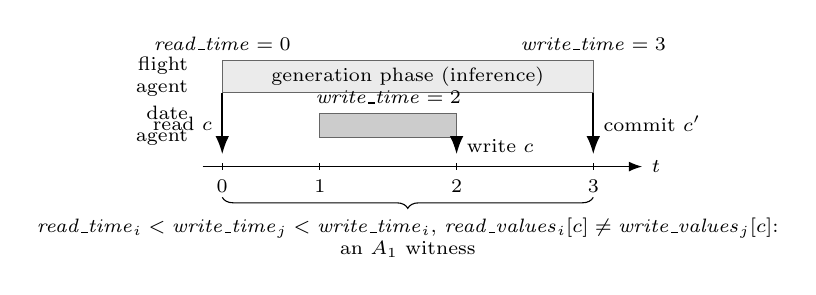
\begin{tikzpicture}[x=0.62cm,y=0.52cm,font=\scriptsize,>=Latex]
  % time axis
  \draw[->] (0,0) -- (9.0,0) node[right]{$t$};
  \foreach \x/\l in {0.4/0,2.4/1,5.2/2,8.0/3} {\draw (\x,0.08)--(\x,-0.08) node[below]{\l};}
  % flight agent
  \node[anchor=east,align=right] at (-0.1,2.2) {flight\\agent};
  \draw[fill=black!8,draw=black!60] (0.4,1.8) rectangle (8.0,2.6);
  \node at (4.2,2.2) {generation phase (inference)};
  \draw[->,thick] (0.4,1.8) -- (0.4,0.3) node[midway,left]{read $c$};
  \node[anchor=south] at (0.4,2.6) {$\rt=0$};
  \draw[->,thick] (8.0,1.8) -- (8.0,0.3) node[midway,right]{commit $c'$};
  \node[anchor=south] at (8.0,2.6) {$\wt=3$};
  % date agent
  \node[anchor=east,align=right] at (-0.1,1.0) {date\\agent};
  \draw[fill=black!20,draw=black!60] (2.4,0.7) rectangle (5.2,1.3);
  \draw[->,thick] (5.2,0.7) -- (5.2,0.3) node[midway,right]{write $c$};
  \node[anchor=south] at (3.8,1.3) {$\wt=2$};
  % witness brace
  \draw[decorate,decoration={brace,amplitude=4pt,mirror}] (0.4,-0.75) -- (8.0,-0.75)
    node[midway,below=4pt,font=\scriptsize,align=center]{$\rt_i<\wt_j<\wt_i$,\ $\rv_i[c]\neq\wv_j[c]$:\\an \A1 witness};
\end{tikzpicture}
\caption{The read--generate--commit window. Logical time is the length of the
operation log. Operation $i$ (flight agent) reads $c$ at $\rt_i=0$; operation
$j$ (date agent) commits a different value to $c$ at $\wt_j=2$, inside $i$'s
window; $i$ commits at $\wt_i=3$ grounded in the superseded read ($L_1$
re-validates the read set at $\wt_i$ and discards the generation).}
\label{fig:window}
\end{figure}

\subsection{Why existing theory does not operationalize these failures}
\label{sec:why-classical-fails}
Hardware models~\cite{Lamport1979SC,HerlihyWing1990}
presuppose bounded latency and static access sets; database isolation
theory~\cite{BerensonEtAl1995,Adya1999,AdyaLiskovOneil2000} supplies the
anomaly-by-anomaly method we follow but holds the read set under lock or
snapshot for the transaction's lifetime; replicated-storage
consistency~\cite{LloydEtAl2011COPS}
treats operations as discrete events with summarizable signatures. The agent
regime has unbounded generation latency, a mutable tool registry, and
irreversible effects, so the cascading-abort machinery of database
recovery, which assumes effects can be undone, is exactly what fails.

\subsection{Contributions}
\label{sec:contributions}
We claim no new concurrency theory; each anomaly below is a classical one,
and we say which. The contribution is the operational port of four of them to
agent runtimes, its mechanization at stated assurance levels, and an
evaluation that measures the gap between each predicate and the harm it
tracks, including the part of the harm that is not a concurrency anomaly.

\smallskip\noindent\textbf{(C1) A catalog with classical names, and what it
leaves out} (\cref{sec:anomalies}). Four history predicates in
\TLA{}---stale generation (\A1), phantom tool (\A2), causal cascade (\A3),
tool-effect reordering (\A6)---each with a TLC witness and its classical
counterpart: a failed backward validation~\cite{KungRobinson1981OCC}, a
dangling capability reference, recoverability with externalization as the
commit point~\cite{BernsteinHadzilacosGoodman1987}, and order preservation
of external effects. \Cref{thm:corc} (TLAPS, \TlapsCommitOrder{}
obligations) places \A1-freedom among the classical classes exactly, as a
conditional guarantee whose hypotheses (per-agent non-overlap,
read-before-commit, faithful records) are stated, checked on every committed
record, and violated by one deployed construct we name. Two predicates stand
outside the catalog, each for a stated reason: the \emph{residue predicate}
\Rp{}---an irreversible effect is out while ordinary later writes have revised
the state it was derived from; not an anomaly, it fires in correct sequential
executions, but the harm no commit-time discipline reaches, decided on the
records by argument provenance, and on the live study \A1 and \Rp{} partition
the outcome column (\cref{sec:residue})---and the \emph{duplication predicate}
$D$---one node's irreversible effect is out twice, the shape a deployed
resumption path produces, a property of the executor's replay semantics
rather than of the window, stated with its witness and the guard that
excludes it (\cref{sec:dup}).

\smallskip\noindent\textbf{(C2) A lattice, realized at stated bounds}
(\cref{sec:lattice}). The $2^4$ exclusion lattice is trivial; what is not is
that every point is inhabited by a checked runtime configuration
(\LatticeRuns{} TLC runs, no mismatch, at two agents, two cells, two
operations and, for the safety half, two values), that one chain
$L_0\subsetneq\dots\subsetneq L_4$ has a verified realizing runtime at every
level, and that the basis ledger composes with every point without
disturbing its verdict (\LatticeThirtyTwoRuns{} further runs).

\smallskip\noindent\textbf{(C3) Verified disciplines, verified detectors, and
exactly which bytes were measured} (\cref{sec:mechanization}). Under two
enumerated axioms and three enumerated stubs, with no \texttt{assume} or
\texttt{admit}: detectors sound and complete against their specifications,
two concurrent $L_1$ stores proved window-free under a verified
reader--writer lock, and $L_2$ (output commit), $L_3$ (commit-order
sequencing) and $L_4$ (validation at dispatch) runtimes whose verified files
are, byte for byte, the files the runtime compiles (a gate checks the
identity); the $L_1$, $L_2$ and $L_4$ bytes are the ones measured\ifnum\ToolNodeVerifiedAvailable=1 , and
so are the $L_3$ bytes\else{} and the $L_3$ replay through its bytes is
\Pending{step 15}\fi. \ifnum\VerifiedScorerAvailable=1 The \A1 verdict of every table
is the verified detector executing, behind one interning wrapper we list in
the trust base; every published cell was rescored through it
(\VerifiedScorerCells{} cells, \VerifiedScorerTraces{} traces,
\VerifiedScorerProblems{} disagreements).\else The \A1 verdict of the
published tables was taken by a hand-written port gated against the verified
predicate on every cell; the verified detector is compiled into the scorer
and the rescoring of every cell through it is \Pending{runner step
14}.\fi{} \Cref{tab:assurance} labels every claim with its assurance level
(checked model, verified decision procedure, verified bytes, unverified port,
open) and names each correspondence between \TLA{} definition, Verus
restatement, executed code and scorer, with its hypothesis and the gate that
checks it. Of \VerusCurated{} obligations, \VerusLoadBearing{} bear a
deployed or measured artifact and \VerusScaffold{} are scaffolding
(supplement \S\,S); the count is an inventory, not a result.

\smallskip\noindent\textbf{(C4) An evaluation scored on outcomes, not flags,
with its own confounds measured} (\cref{sec:eval}). For each discipline we
report the anomaly it excludes, the harm that remains, and the price: on the
live LangGraph study the $L_1$ residue is \Rp{} in $1$--$65\%$ of sessions
per family and arm at the $150$\,ms offset ($0$--$73\%$ in single runs),
on three API families and in two implementations of $L_1$ between which
three interleaved replications detect no difference, decided on the
records; the basis ledger with a compensator removes it on the store
($0/2{,}100$ across both ledger arms and four runs), and in a world with a
downstream consumer and a compensator the world refuses at an injected
rate, the refused share ends wrong or empty and $1$--$10\%$ of sessions are
misreported as repaired (\cref{sec:ledger-world});
on $1{,}000$ seeded cascades per depth, output commit removes exposure
exactly when the review precedes the release and refuses the retraction
otherwise; per sound committed operation, snapshot isolation costs
$+0.4$--$11.1\%$ and pessimistic locking $+1.2$--$97\%$ in tokens. Where
the design limits what a difference can mean we quantify the confound on
the receipts and say which comparisons it voids.

\smallskip\noindent\textbf{(C5) Where the preconditions occur} (\cref{sec:prevalence}).
A census of \CensusRepos{} public LangGraph repositories (\CensusSites{} graph
sites) finds no confirmed co-scheduled reader and writer of a last-value
channel (eight sites unresolved; a bracket of none to about half)---a
negative result for \A1's structural precondition, which we report as
one---while
a released tool executor dispatches a model-emitted, order-dependent pipeline
concurrently on $\ToolNodeGptBatched/\ToolNodeGptBatched$ turns of one backbone
and never on another, which is the case for \A6.

\smallskip\noindent\textbf{What this paper does not establish.} No
production prevalence for any anomaly: every occurrence figure is a race our
harness opened or a rate on our own workloads, and the census measures how
public code is written, not how often it runs. The instrumentation and the
Python harnesses are not verified (\cref{sec:trust}), and the refinement of
the deployed concurrent stores to their abstract machines is open. A verified
arm's zero is a theorem executing, not evidence, so the evaluation leads with
costs and with counts that read no runtime flag.

% ============================================================================
% sec/02-model.tex
% ============================================================================
\section{Runtime model}
\label{sec:model}

A system consists of a finite set of agents $A$, a shared memory $M$ mapping
cells to values with a distinguished sentinel $\mathrm{NULL}$, and a shared
registry $R$ of available tools. An agent executes a sequence of
\emph{operations}, each in three phases: a \emph{read} phase that captures the
values of a chosen subset of cells (the operation's $\rs$) together with the
registry contents ($\rreg$), stamping the read with the current log length as
$\rt$; a \emph{generation} phase, dominated by inference latency and not
treated as instantaneous; and a \emph{write} phase that atomically appends a
record to the log, installing the planned writes ($\ws$, $\wv$), the selected
tool ($\pt$) and the registry at commit ($\wreg$), stamped $\wt$. The log
length is a logical clock~\cite{Lamport1978TimeClocks}; a history $h$ is the
log, $h\in\mathrm{Seq}(\fld{OpRecord})$. The specification is
\texttt{Memory.tla}.

\smallskip\noindent\emph{Store axiom.} A read returns the latest committed
value at or before its read time (stamps are log lengths, so no write
shares a stamp with a read and ``after'' is the strict inequality of
\cref{def:a1}). TLC confirms this and the two hypotheses
below as invariants of \texttt{Memory.tla} over all
\CommitOrderMemoryStates{} reachable states at the checked bounds
(\cref{sec:a1}).

\smallskip\noindent\emph{Per-agent non-overlap; read before commit.} Two
operations of one agent do not overlap in $[\rt,\wt]$; every operation reads
strictly before it commits. Both are invariants of the model, and both are
load-bearing for \cref{thm:corc} and for the detector transcription of
\cref{sec:verus-detectors}. A framework that runs one node as several parallel
instances under one name (LangGraph's \texttt{Send} fan-out) violates the first
and is outside the model; \cref{sec:prevalence} counts how often that shape
appears in public code.

\smallskip\noindent\emph{Determinism is not assumed by the theorems.} Every
mechanized result ranges over recorded histories with write values free. Under
sampling, a value mismatch need not change the downstream decision, so the
\A1 detector is a sound candidate screen that over-reports by a factor
\cref{sec:live-a1} measures (materiality). Durable-execution engines take the same
stance~\cite{BurckhardtEtAl2021Durable}: replay is deterministic because every
non-deterministic step's result is recorded, not because the step is.

\smallskip\noindent\emph{Atomic commit is at the record level.} External
effects are outside the store and are governed separately: their order by
\A6 and $L_3$, their release relative to a still-retractable basis by \A3 and
$L_2$. At-most-once externalization is a hypothesis of this model; it is
stated as the predicate $D$ of \cref{sec:dup}, checked on every committed
record (\HypDuplicateEffects{} duplicate emissions among \HypExternalEffects{}
externalized effects), and violated by one deployed resumption path we
reproduce.

\smallskip\noindent\emph{No replication; no one runtime.} The memory is one
logical store (split view under replication, \A4, is formalized in
supplement \S\,J and plays no role in the lattice), and the model derives
from no one runtime: LangGraph is driven through it live
(\cref{sec:live-a1}); three others are placed informally (supplement \S\,D).

% ============================================================================
% sec/03-catalog.tex
% ============================================================================
\section{The anomaly catalog}
\label{sec:anomalies}

Four anomaly predicates over histories are formalized in \TLA{}
(\texttt{Anomalies.tla}); each has a TLC witness at $|A|{=}2$,
$|\fld{Cells}|\le 2$, $\fld{MaxOps}\le 4$, reproduced by the artifact's
\texttt{reproduce.sh}. Each predicate's classical counterpart and the
regime feature that forces the port are named in its subsection and
tabulated in supplement \S\,R. The numbering
($A_1, A_2, A_3, A_6$) is kept from the public artifact (an earlier $A_5$
was subsumed by \A1); \cref{sec:residue} defines, outside the catalog, the
predicate for what the four leave behind.


\subsection{\A1: stale generation}
\label{sec:a1}
\begin{definition}[Stale generation]
\label{def:a1}
A history $h$ exhibits \emph{stale generation} when there exist
$i\neq j$ with $h[i].\fld{agent}\neq h[j].\fld{agent}$ and
$c\in h[i].\rs\cap h[j].\ws$ such that
\[
  \begin{gathered}
  h[i].\rt < h[j].\wt < h[i].\wt\\
  \text{and}\quad h[i].\rv[c] \neq h[j].\wv[c].
  \end{gathered}
\]
\end{definition}

\noindent\emph{Witness.} TLC finds a five-state counterexample: $a_2$ reads
$c_1=\mathrm{NULL}$ at $\rt=0$; $a_1$ commits $c_1=v_1$ at $\wt=1$; $a_2$
commits at $\wt=2$ with $\rv[c_1]=\mathrm{NULL}$.

\smallskip\noindent\emph{Classical placement.} The minimal witness is a single
read--write antidependency from $i$ to $j$, serializable in the order $i;j$,
and none of Adya's proscribed phenomena~\cite{Adya1999}; TLC exhibits such a
history (claim \texttt{A1OnlyOnNonSerializable}, violated as expected). \A1
is therefore not an isolation anomaly in the classical sense. Its
\emph{absence} is nevertheless a classical correctness class, and we state
which one at the level at which the theorem holds.

\begin{definition}[Commit-order read consistency]
\label{def:corc}
A history is \emph{commit-order read consistent} when every operation read, for
every cell in its read set, exactly the value it would have read had it
executed atomically at its own commit point: for all $i$ and $c\in h[i].\rs$,
$h[i].\rv[c]$ is the value of the latest write to $c$ with
$\wt<h[i].\wt$, or $\mathrm{NULL}$ if there is none.
\end{definition}

Writes are installed in commit order in any case, so \cref{def:corc} is
value-level equivalence, on the reads, to the serial execution in commit
order. It is the value-level analogue of Weikum and Vossen's
commit-order-preserving serializability~\cite{WeikumVossen2001} and not that
condition itself, which is conflict-based; under value-unique writes the two
coincide on reads (view equivalence~\cite{Papadimitriou1979}).

\begin{theorem}[\A1-freedom implies commit-order read consistency]
\label{thm:corc}
Let $h$ satisfy the store axiom, read-before-commit and per-agent non-overlap.
If $h$ has no \A1 witness, then $h$ is commit-order read consistent.
\end{theorem}

The proof (\texttt{CommitOrder.tla}; TLAPS, \TlapsCommitOrder{} obligations,
no omitted step) is Kung and Robinson's backward-validation argument run
against our definitions: if some operation's read of $c$ disagrees with the
latest write to $c$ before its commit, that write lies inside the operation's
window, was made by another agent (one agent's operations do not overlap), and
wrote a different value---an \A1 witness. Fifteen TLC verdicts
(\texttt{check\_commitorder.sh}) fix what the statement says, and all
reproduce: over all \CommitOrderHistories{} histories of length at most
three the implication holds; it is not vacuous; it fails when either
droppable hypothesis is removed; the relational definitions equal
\texttt{Memory.tla}'s and a literal serial replay; the three hypotheses are
invariants of the operational model over \CommitOrderMemoryStates{} reachable
states; and the converse fails in exactly one shape---a value overwritten and
then restored inside the window fires \A1 although the history is
commit-order read consistent. The predicates nest strictly:
\[
  \neg\text{CORC} \;\Longrightarrow\; A_1 \;\Longrightarrow\; \text{validation fails}.
\]
\emph{Reach.} The theorem is a conditional guarantee over faithful histories
that satisfy its three hypotheses; it says nothing about serializability of
an application, about effects, about reads the instrumentation did not
declare, or about a runtime that violates per-agent non-overlap---LangGraph's
\texttt{Send} fan-out, several instances under one agent name, is outside
the model (\cref{sec:model}). On the committed data both droppable
hypotheses hold---\HypSameAgentOverlaps{} same-agent overlapping windows and
\HypReadBeforeCommitViolations{} reads not before their commit in
\HypRecords{} records over \HypTraces{} traces (\texttt{hypothesis\_gates.py},
a gate that fails on the first violation; the live sessions commit once
per agent, so the pilot's multi-operation traces are where the first can
fail)---and a runtime can enforce the first by refusing a second operation
of an agent whose window is open. The
converse shape is a false positive of $L_1$, priced in discarded
generations; on the live records it occurs in \HypRestored{} of
\HypAOneWitnesses{} \A1 witness pairs. Two corollaries are mechanized with
the theorem: the classical lost update (P4 of Berenson et
al.~\cite{BerensonEtAl1995}) is an \A1 witness in which the stale reader
also writes the cell it read, so $L_1$ excludes it; a \emph{blind}
overwrite---a write by an operation that never read the cell---is not an
anomaly in isolation theory and is outside the catalog, and it is the kind
of the one in-the-wild bug we reproduce (\cref{sec:prevalence}) and of a
revision that lands \emph{after} the reader's commit (\cref{sec:live-a1}).

\subsection{\A2: phantom tool}
\label{sec:a2}
\begin{definition}[Phantom tool]
\label{def:a2}
$h$ exhibits a \emph{phantom tool} when for some $i$,
\[
  \begin{gathered}
  h[i].\pt\neq\mathrm{NULL},\\
  h[i].\pt\in h[i].\rreg,\\
  h[i].\pt\notin h[i].\wreg.
  \end{gathered}
\]
\end{definition}
An agent selects a tool from the registry it read; the registry mutates
during generation; the commit emits a call to a capability that no longer
exists. TLC's witness has four states. \emph{Tool validity}, canonically, is
membership of the (identifier, signature) pair. \Cref{def:a2} is stated over
identifiers, the \TLA{} registry being a set of them; the Verus restatement
of \cref{sec:l4} maps identifiers to signatures and fires additionally when
a tool is re-signed under its old name. The two coincide under the encoding
the executable dispatcher uses, in which re-signing is removal of the old
pair and insertion of a fresh one; the scorer and the $L_4$ dispatcher
decide the pair form, and \cref{tab:assurance} records the correspondence
as an encoding, not a proof. A tool the agent names that was never in
$\rreg$ (a hallucinated call) is not \A2 and not in the catalog.

\subsection{\A3: causal cascade}
\label{sec:a3}
When an operation is retracted in a compensating (saga-style) runtime, any
operation that read a value it produced is grounded on a basis no surviving
commit supports. The classical remedy, cascading abort, flags the dependent
aborted. In the agent regime that remedy fails in a specific way: if the
dependent's tool effects have already been issued, the flag changes nothing
that reached the world. The cataloged predicate is therefore stated over
externalization.

\begin{definition}[Causal cascade]
\label{def:a3}
Let each record carry $\fld{aborted}$ and $\fld{externalized}$ flags and a
predecessor set $\fld{preds}$ (the operations whose committed writes it
observed, transitively closed). $h$ exhibits a \emph{causal cascade} when for
some $j,p$:
\[
  h[j].\fld{externalized}\;\wedge\;p\in h[j].\fld{preds}\;\wedge\;h[p].\fld{aborted}.
\]
\end{definition}
The surviving-dependent form, $\neg h[j].\fld{aborted}\wedge p\in
h[j].\fld{preds}\wedge h[p].\fld{aborted}$, is kept beside it as
\textsc{CascadeUnpropagated}; a cascading abort falsifies that form by
flagging $j$ after $j$'s effects are out, and \cref{sec:l2-eval} measures the
separation on runnable arms.

\smallskip\noindent\emph{Prevention is output commit, and output commit has a
residue.} Under \cref{def:a3} a runtime must hold an operation's effects
(output commit, in the sense of optimistic
recovery~\cite{StromYemini1985OptimisticRecovery}) until
every operation in its closure has released its own, and must refuse to
retract an operation whose effects are out. The first clause is prevention;
the second keeps the predicate false by refusing to set the flag it reads,
which we do not count as prevention---a refused retraction is a basis someone
wished to withdraw after release, the ordinary rule that a committed
transaction cannot abort---and \cref{sec:l2-eval} counts its residue beside
the zero.

\smallskip\noindent\emph{What the detector decides.} A trace without
provenance fields cannot decide \cref{def:a3}. What it can decide is an
\emph{unsupported read}---a committed read of a value that no surviving
committed write produced at or before the read. The verified
\texttt{detect\_a3} decides exactly that screen, and its relation to
\cref{def:a3} is five mechanized facts (supplement \S\,G): it is not sound
in general (a value collision hides the aborted writer), it is sound under
value-unique writes, the hypothesis black-box isolation checkers also
need~\cite{Aphyr2020Elle,TanEtAl2020Cobra}, it holds along chains, it is not
complete, and it is blind to relabeled effects. We therefore claim
\cref{def:a3} only where the hypothesis holds, and check it: value-unique
writes hold by construction in the synthetic cascades (distinct value ranges
per writer) and in all \HypLiveLtwoSessions{} live replay sessions
(\HypLiveLtwoCollisions{} collisions), the two data sets the detector scores;
they fail in \HypCollisionCells{} cells of the pilot and occurrence-study
traces, where only \A1 is scored. A recorder that stamps each written value
with its writer's operation identifier makes the hypothesis a system
invariant.

\subsection{\A6: tool-effect reordering}
\label{sec:a6}
Each record additionally carries an issuance order $\fld{io}$ and a commit
order $\fld{co}$ over its external effects; $\ws$ and $\wv$ derive from
$\fld{co}$.
\begin{definition}[Tool-effect reordering]
\label{def:a6}
$h$ exhibits \emph{tool-effect reordering} when for some $i$,
\[
  \begin{gathered}
  |h[i].\fld{io}|\ge 2,\quad h[i].\fld{co}\neq h[i].\fld{io},\\
  h[i].\fld{co}\ \text{is a permutation of}\ h[i].\fld{io}.
  \end{gathered}
\]
\end{definition}
The minimal witness (three states, one agent, two cells) is benign over store
cells, where writes to distinct cells commute; the predicate names an anomaly
only under the reading in which each element of $\fld{io}$ is an external
effect whose order an observer can see. It over-reports on commuting effects
and, because it requires a permutation, is silent on dropped and duplicated
effects; \cref{sec:limitations} exhibits the duplicated case in a deployed
framework.


\subsection{Snapshot insufficiency}
\label{sec:snapshot}
$L_1$ is not a snapshot guarantee: ``reads reflect memory at read time''
is the store axiom of \cref{thm:corc}, holds on every reachable log, and
TLC exhibits a history satisfying it on which \A1 fires
(\texttt{MC\_A1\_struct}; supplement \S\,B). The live instance is a runtime
that pins a consistent snapshot per node---LangGraph's superstep---and has
not thereby obtained $L_1$ (\cref{sec:live-a1}).

\subsection{What the catalog leaves: the residue predicate}
\label{sec:residue}
Every predicate above is decided at or before an operation's commit, and a
discipline that excludes all four still leaves a harm the live study measures
in $1$--$65\%$ of sessions per family and arm on the API families
(\cref{sec:live-a1}): the
external effect a commit released is irreversible, while the state it was
derived from is ordinary revisable state that any later operation may
overwrite. This is not a concurrency anomaly. It fires in correct sequential
executions---book against the date known at commit, then be contradicted by
a legitimate revision---and classical isolation has no name for it because a
committed transaction's inputs are final by definition; the nearest notions
are view maintenance~\cite{GuptaMumick1995ViewMaint} with the view outside
the system, and the saga's compensation~\cite{GarciaMolinaSalem1987Sagas}. We
define it because an evaluation scored on outcomes needs a predicate for the
outcome's other half, and keep it outside the catalog and the lattice.

Each operation record carries a \emph{basis}, the (cell, value) pairs its
external effect was derived from, and an $\fld{obligation}$ flag. The basis
is recovered by \emph{argument provenance}: a read value that appears
verbatim among the effect's arguments is part of its basis, and nothing is
declared by the agent. This is why-provenance~\cite{BunemanEtAl2001Why}
restricted to copying, with that tradition's known limit: a value that
reaches the effect through a computation leaves no basis, so the extractor
under-reaches and never over-reports. In the model the basis is a
nondeterministic subset of the read values, so every extractor is covered.

\begin{definition}[Residue predicate]
\label{def:residue}
$h$ exhibits a \emph{superseded-basis effect} (\Rp{}; \texttt{NoA7} in the
artifact) when for some $i$, $h[i].\fld{externalized}$,
$\neg h[i].\fld{obligation}$, and for some $(c,v)\in h[i].\fld{basis}$ the
\emph{latest} write to $c$ committed after $h[i].\wt$ wrote a value other
than $v$:
\[
  \begin{gathered}
  \exists j:\ c\in h[j].\ws \;\wedge\; h[j].\wt > h[i].\wt\\
  \qquad\wedge\; h[j].\wv[c]\neq v\\
  \wedge\ \forall k:\ (c\in h[k].\ws \wedge h[k].\wt > h[i].\wt)\\
  \qquad\qquad\Rightarrow h[k].\wt \le h[j].\wt.
  \end{gathered}
\]
\end{definition}

\A1 and \Rp{} partition ``an effect is out on a basis the state no longer
holds'' by whether the superseding write committed inside the operation's
window or after its commit; a value overwritten and then restored fires
neither, and \Rp{} carries no agent conjunct because the obligation is owed
whoever supersedes. On the live data the partition is exact
(\cref{tab:live}): $A_1 + R = 100$ in every unguarded cell, and under $L_1$
the residue is entirely \Rp{}. The identity is not evidence for the
extractor: on a workload that copies the date verbatim into the booking it
holds whenever the extractor recovers the basis at all, and it recovers
\HypBasisRecovered/\HypBookings{} because the booking tool takes the date as
a structured argument; we keep it as a gate (\texttt{a7\_rescore
-{}-check}) and state the extractor's blind spot in \cref{sec:limitations}.
TLC's witness has five states and is not an \A1 witness: an operation reads
$c_1=\mathrm{NULL}$ and commits an effect with basis
$\{(c_1,\mathrm{NULL})\}$, released at commit; a later operation commits
$c_1=v_1$.

\smallskip\noindent\emph{What remains after release (a remark, not a
result).} Under the \emph{open-world hypothesis}---the store accepts, at
any time after an effect $e$ with basis $B$ is released, a write to a cell
of $B$ by an operation that does not depend on $e$---two things are
immediate and fix what a discipline can promise. (i)~Some execution
supersedes $B$ while $e$ is out, because the write is admitted after a
release that cannot be recalled. (ii)~If obligations are never cleared,
$\neg R$ holds in every reachable state iff, in every execution, $e$'s
obligation is set in the same step as, or before, every step that completes
the other conjuncts of \cref{def:residue} (the superseding commit for a
released effect; the release for an effect superseded while held), because
\cref{def:residue} is ``superseded and not owed'' and a monotone flag set by
the first such step stays set. So a discipline can promise not a current
basis but an obligation registered atomically with the step that completes
the witness, which the ledger of \cref{sec:ledger} does at both steps (the
executable ledger clears a discharged obligation and re-arms the basis;
never-cleared is the model's hypothesis).
Dropping the hypothesis is not free: freezing the cells of $B$ until the
effect is acknowledged is a lock held past commit, with the pessimistic
column of \cref{tab:cost} as its price floor; output commit (\cref{sec:a3})
holds effects only until their \emph{causal} basis is externalized, a finite
condition. What a registered obligation buys in the world is a property of
the compensator and is measured, not proved (\cref{sec:ledger-world}).

\subsection{What the model assumes about effects: at-most-once, as a predicate}
\label{sec:dup}
The model externalizes an operation's effects once, at commit. LangGraph's
\texttt{interrupt} resumes a node by re-executing it from its start, so an
irreversible effect issued \emph{before} the gate is emitted again after it,
with different arguments when the shared value was revised during the gate
(\cref{sec:prevalence}; \HypInterruptEmissions{} emissions of one pre-gate
effect in the probe). Rather than record this as a limitation we state the
hypothesis as a predicate over the effect stream: $D$ holds when two
emissions carry the same node's effect, and $D^{\neq}$ when they also differ
in their arguments. A five-action \TLA{} module (\texttt{Duplication.tla}:
issue, gate, resume-from-start, finish, revise) reaches $D$ in
\DupWitnessDepth{} steps and $D^{\neq}$ in \DupDivergentDepth{}, and with an
idempotency key per (node, effect) TLC finds neither over \DupDedupStates{}
states exhaustively, with exactly one effect out per finished node. $D$ is
kept outside the catalog and the lattice like \Rp{}: its carrier, the effect
stream, is disjoint from the four disciplines', which therefore neither
create nor remove it. On the committed records \HypDuplicateEffects{} of
\HypExternalEffects{} externalized effects were emitted twice
(\texttt{hypothesis\_gates.py}, H5).

% ============================================================================
% sec/04-lattice.tex
% ============================================================================
\section{The lattice and one chain through it}
\label{sec:lattice}

A consistency model is a predicate over histories, characterized by the set of
anomalies it excludes~\cite{Adya1999}. With
$\mathcal{A}=\{A_1,A_2,A_3,A_6\}$ the design space is the Boolean lattice
$\langle 2^{\mathcal{A}},\subseteq\rangle$: sixteen points, bottom
$\emptyset$ admitting everything, top $\mathcal{A}$ admitting nothing
(drawn in supplement \S\,L). We name five points on one maximal chain,
\[
  L_0\equiv\emptyset,\;
  L_1\equiv\{A_1\},\;
  L_2\equiv\{A_1,A_3\},\;
  L_3\equiv\{A_1,A_3,A_6\},\;
  L_4\equiv\mathcal{A},
\]
chosen on operational grounds (\A1 first because it is the basic
read--generate--commit failure; \A2 last because registry stability across
the operation lifetime is the costliest single requirement); the other
twenty-three linearizations are equally valid and the lattice, not the chain,
is primary. The residue predicate \Rp{} is not a generator: it is not an
anomaly, and its answer, the basis ledger $\ell$ of \cref{sec:ledger},
composes with any point.


\subsection{What is and is not a result}
The chain's inclusions are definitional and its strictness needs one witness
per step; neither is a result. What requires work is \emph{realizability}: a
runtime configuration that excludes exactly each point's anomalies, and for
the five named points a verified realizing runtime---established here by
bounded model checking at two agents, two cells and two operations (three
for \A3), one value for the witness half and two for the safety half, and
claimed at exactly those bounds; histories of that length exercise every
predicate's minimal witness and nothing longer, and the unbounded statement
exists only for the top point, as the Verus product of
\cref{sec:composition}.

\subsection{All sixteen points, mechanically; the ledger composes}
\label{sec:lattice16}
\texttt{Guarded.tla} extends the runtime with four commit-time disciplines,
each enabled by a Boolean constant and each acting on its own carrier: $G_1$,
read-set validation (an operation whose read set was overwritten after its
read may not commit); $G_2$, registry validation (a planned tool no longer in
the registry may not be dispatched); $G_3$, causal tracking with output commit
(an operation records the closure of committed writers whose values it read,
may not commit while any is aborted, externalizes only once its closure has
externalized, and once externalized is irrevocable; a retraction cascades to
every unexternalized dependent); $G_6$, commit-order sequencing (effects
externalize in issuance order). The carriers are disjoint---read set and write
times; registry and planned tool; closure and abort flags; issuance and commit
orders---so enabling one guard neither creates nor removes another anomaly,
and the matrix confirms it on every combination.

For each of the sixteen guard sets $S$ and each anomaly $a$, TLC checks
$R(S)\models\neg a$: for $a\in S$ the invariant must hold exhaustively, for
$a\notin S$ it must be violated. All \LatticeRuns{} runs match
(\texttt{lattice16.sh}; $|A|{=}2$, $|\fld{Cells}|{=}2$, $|\fld{Values}|{=}1$,
$\fld{MaxOps}{=}2$, symmetry on agents and cells; the $32$ safety runs are
exhaustive over \LatticeSafeStatesMin{}--\LatticeSafeStatesMax{} distinct
states). Because \textsc{CausalCascade} ranges over flags and predecessor
sets and never over cells, the sixteen \textsc{NoA3} points are rechecked at
$\fld{MaxOps}{=}3$ with one cell, where a transitive cascade first becomes
reachable: \LatticeMaxOpsThreeRuns{}/\LatticeMaxOpsThreeRuns{} match. A
single-value domain makes \cref{def:a1}'s value conjunct vacuous on non-null
reads; the safety half re-run at $|\fld{Values}|{=}2$ on the current model
stays safe (\LatticeVtwoOutcome), and a targeted check shows the
non-null-read witness class needs both a second value \emph{and} a third
operation (supplement \S\,L). Every point is thus inhabited by a runtime
that prevents exactly its avoidance set, at these bounds; the Verus product
of the $L_2$, $L_3$ and $L_4$ models (\cref{sec:composition}) mechanizes the
top point without a bound.

\smallskip\noindent\emph{The ledger composes.} \texttt{Guarded5.tla} adds a
fifth constant $G_7$, the basis ledger of \cref{sec:ledger}, which refuses
nothing and writes only the basis and obligation fields.
\texttt{lattice32.sh} runs all \LatticeThirtyTwoRuns{} combinations of the
five constants against the four anomalies and \Rp{} at the same bounds. The
$64$ anomaly cells with $G_7$ on return the verdicts of \texttt{lattice16.sh}
one for one, so the ledger disturbs no point of the lattice; \Rp{} is
reached without $G_7$ in a five-state trace at every point and excluded
with $G_7$ at every point (exhaustive; \NoAsevenStates{} distinct states at
the bottom point, \NoAsevenStatesGthree{} with output commit, where a held
effect can be superseded before its release); no run mismatches its
expectation.

% ============================================================================
% sec/05-mechanization.tex
% ============================================================================
\section{Mechanization}
\label{sec:mechanization}

Three tools carry the development, at assurance levels \cref{tab:assurance}
labels claim by claim. TLC checks the witnesses, the lattice and ledger
matrices and the fifteen \cref{thm:corc} verdicts (bounded, exhaustive
within bounds). TLAPS proves \cref{thm:corc} (\TlapsCommitOrder{}
obligations), a coherence check of the chain definitions
(\texttt{Hierarchy.tla}, \TlapsHierarchy{}) and a same-agent exclusion lemma
(\texttt{A1LowerBound.tla}, \TlapsLowerBound{}); only the first is a
substantive result. Verus~\cite{Lattuada2023Verus} carries the substantive
mechanization: \VerusCurated{} obligations (\VerusFull{} counting four helper
files), zero errors, no \texttt{assume} or \texttt{admit} in any proof body,
regenerated by \texttt{verus\_count.sh} against a pinned build
(\texttt{verus-version.txt}; a newer verifier makes proof files stop
compiling rather than fail, which the counter reports as such). Of these,
\VerusLoadBearing{} bear a deployed or measured artifact's safety claim and
\VerusScaffold{} are scaffolding (superseded refinements, the $A_4$ model,
the model-only Verus mirror of \texttt{Guarded.tla}); supplement \S\,S
inventories every file.



\begin{table*}[t]
\centering
\caption{Every claim at its assurance level. \emph{Model}: checked by TLC
within bounds; \emph{proof}: TLAPS or Verus, no \texttt{assume}/\texttt{admit};
\emph{bytes}: the verified code is the code measured; \emph{port}: unverified
code gated against a verified artifact on the committed data; \emph{open}:
stated, not established. Correspondences name the hypothesis under which two
formalizations agree and the gate (\texttt{harness/macaudit/}) that checks it.}
\label{tab:assurance}
\scriptsize
\setlength{\tabcolsep}{4pt}
\begin{tabular}{@{}p{2.7cm}p{1.8cm}p{2.4cm}p{3.4cm}p{6.7cm}@{}}
\toprule
Claim & Definition & Proof / check & Executed by & Correspondence, hypothesis, gate; status \\
\midrule
Anomaly witnesses, lattice realizability & \TLA{} & TLC, $|A|{=}2$, $\le2$ cells, $\le2$ values, $\mathrm{MaxOps}\le4$ (witnesses), $\le3$ (matrix) & --- & \textbf{model}: bounded; \LatticeRuns{}$+$\LatticeMaxOpsThreeRuns{}$+32$ two-value safety runs \\
\cref{thm:corc} & \TLA{} & TLAPS \TlapsCommitOrder{} & --- & \textbf{proof}; hypotheses H1--H3 are model invariants (TLC) and H1 is checked on all \HypRecords{} committed records (\texttt{hypothesis\_gates}: \HypSameAgentOverlaps{} violations) \\
\texttt{detect\_a1} sound \& complete & Verus spec & Verus & scorer: \ifnum\VerifiedScorerAvailable=1 the verified bytes (\texttt{detect\_a1\_exec.rs}) behind an interning wrapper\else port (gated); the verified bytes wired, rescoring pending\fi{} & \textbf{proof} against the restatement; restatement $=$ \cref{def:a1} under \cref{lem:same-agent} (TLAPS step); \ifnum\VerifiedScorerAvailable=1\textbf{bytes}: every published cell rescored through them (\texttt{verified\_scorer\_gate}: \VerifiedScorerProblems{} disagreements); wrapper trusted (xii)\else\textbf{port} on the published cells, gated on every cell (\texttt{predicate\_matrix\_a1}); rescoring through the verified bytes \Pending{step 14}\fi \\
\texttt{detect\_a2} & Verus spec (id, signature) & Verus & $L_4$ dispatcher (bytes); scorer (port) & \textbf{proof} of the detector, \textbf{port} in the scorer; \cref{def:a2} (identifiers) coincides under the re-sign-as-replace encoding; \textbf{encoding stated, not proved} \\
\texttt{detect\_a3} & Verus spec (unsupported read) & Verus & scorer (port) & \textbf{proof} for the screen, \textbf{port} in the scorer; $=$ \cref{def:a3} under value-unique writes, which hold on every scored trace (\texttt{hypothesis\_gates}: \HypLiveLtwoSessions{} sessions, \HypLiveLtwoCollisions{} collisions) \\
\texttt{detect\_a6} & Verus spec & Verus & scorer (port) & \textbf{proof} of the detector, \textbf{port} in the scorer; single-record equivalence to \cref{def:a6} \\
$L_1$ stores window-free & Verus & Verus (lock predicate) & pilot (bytes); live \emph{verified} arm (bytes via bridge); \emph{validated} arm (application layer) & \textbf{bytes} in the pilot and the verified arm; \textbf{port} in the validated arm; refinement to the abstract machine \textbf{open} \\
$L_2$ output commit & Verus & Verus & \texttt{l2\_exec} (bytes) & \textbf{bytes}; sequential object, caller serializes \\
$L_3$ sequencing & Verus & Verus & \ifnum\ToolNodeVerifiedAvailable=1 \texttt{l3\_exec} (bytes, via \texttt{l3\_server})\else twin (inspection); \texttt{l3\_exec} behind a bridge \Pending{step 15}\fi & \ifnum\ToolNodeVerifiedAvailable=1\textbf{bytes}; bridge trusted (xiii)\else\textbf{port}\fi \\
$L_4$ validation at dispatch & Verus & Verus & \texttt{l4\_exec} (bytes) & \textbf{bytes} \\
\Rp{} on the live records & \cref{def:residue} & --- & \texttt{a7\_rescore} (Python) & \textbf{port}, unverified; independent of the outcome column; extractor coverage \HypBasisRecovered/\HypBookings{} on this workload (no reference set: coverage, not recall) \\
Basis ledger excludes \Rp{} & \TLA{} $G_7$; Verus model & TLC \LatticeThirtyTwoRuns{} runs; Verus \LfiveVerusIntro & probe 303/304 ledger arms (Python, over $L_1$) & \textbf{model} and \textbf{proof}; the executable ledger is a \textbf{port} (harness code); in a world its worth is the compensator's, measured (\cref{sec:ledger-world}) \\
$D$ (at-most-once) excluded by an idempotency key & \TLA{} & TLC: witness, exhaustive with the key & --- & \textbf{model}: bounded (\DupDedupStates{} states); on the records \HypDuplicateEffects/\HypExternalEffects{} duplicates (\texttt{hypothesis\_gates}, H5) \\
\bottomrule
\end{tabular}
\end{table*}

\subsection{Verified detectors, and one transcription gap}
\label{sec:verus-detectors}
The four detectors are verified sound \emph{and} complete against Verus
\texttt{spec} restatements of the \TLA{} predicates (\VerusDetector{}
obligations). \texttt{detect\_a1} is a two-sided equivalence whose
completeness half strengthens each of three nested loop invariants to carry
``no witness in the prefix searched.'' \texttt{detect\_a2} and
\texttt{detect\_a6} are single-record equivalences; \texttt{detect\_a3} is
exact for the flat-trace residue of \cref{sec:a3}.

The restatement is hand-written and checked by inspection, and inspection
found a gap we state rather than hide: the Verus \texttt{OpRecord} carries no
agent field, so its \A1 predicate omits the different-agent conjunct of
\cref{def:a1}, and it decides ``no witness'' when a read value is absent,
where the \TLA{} compares against $\mathrm{NULL}$. Neither matters on the
histories the model admits.

\begin{lemma}[Same-agent exclusion]
\label{lem:same-agent}
Under per-agent non-overlap and read-before-commit, if
$c\in h[i].\rs\cap h[k].\ws$ and $h[i].\rt<h[k].\wt<h[i].\wt$, then
$h[i].\fld{agent}\neq h[k].\fld{agent}$.
\end{lemma}
The lemma is step $\langle2\rangle2$ of the TLAPS proof of \cref{thm:corc}
and the content of \texttt{A1LowerBound.tla}. It makes the Verus predicate
and \cref{def:a1} coincide on every history satisfying the model's invariants;
on a history that violates non-overlap the Verus predicate is strictly
stronger---it over-reports, the safe direction for a detector. The
instrumentation records a value for every read cell, so the absent-value case
does not arise: across all \HypRecords{} committed operation records there
is no read cell without a value and \HypSameAgentOverlaps{} same-agent
overlapping windows (\texttt{hypothesis\_gates.py --check}).

\smallskip\noindent\emph{Which bytes score \A1.} Agreement of three
transcriptions on committed data is testing, not equivalence, and the
earlier version of this paper reported tables scored by a hand-written port
with such a gate. The scorer is now wired to take its \A1 verdict from
\texttt{detect\_a1} itself (its first rescoring pass is the pending receipt
below): the verified exec-mode file
(\texttt{lib\_detect\_a1\_exec.rs}, $9$ obligations, sound and complete
against \texttt{is\_a1\_witness}, the conjuncts of the gated restatement
\texttt{a1\_witness} over (cell, value) pairs in place of a set and a map;
their agreement is checked by inspection and on every cell by the same
gate) is compiled by plain cargo into the runtime crate byte-identical to
the verified source, and a $60$-line wrapper interns cell names and values
injectively to the integers the verified predicate ranges over, drops a
duplicated declared cell (the precondition \texttt{wf\_hist}) and encodes a
read cell without a value as a sentinel no record can carry; the wrapper is
the one unverified piece between the verified bytes and a string-valued
record, trust-base item (xii). The port is kept beside it and the binary
refuses a trace on which the two disagree. \ifnum\VerifiedScorerAvailable=1 Every published \A1 cell was
rescored through the verified bytes: \VerifiedScorerCells{} cells,
\VerifiedScorerTraces{} traces, \VerifiedScorerProblems{} disagreements with
the manuscript's counts and with an independent Definition-1 implementation
(\texttt{verified\_scorer\_gate.py}; receipt committed).\else The rescoring
of every published cell through the verified bytes is \Pending{runner step
14}; until its receipt is committed the tables stand on the gated port.\fi

\subsection{$L_1$: two concurrent stores whose lock is verified, not assumed}
\label{sec:l1}
Three abstract state machines---pessimistic locking, serializable snapshot
isolation (SSI), and default snapshot isolation with its no-write bypass---are
proved \A1-free under sequential interleaving ($40$ obligations; default-SI
conditionally, on workloads with no read-only commit, which is the residual
\cref{sec:pilot} measures). The deployed stores do not rest on these: each is
an exec-mode store whose only access path is \texttt{vstd::rwlock::RwLock},
the reader--writer lock implemented and verified inside the Verus standard
library, carrying the store's invariant as the lock predicate
(\texttt{lib\_si\_concurrent.rs}, $18$; \texttt{lib\_pess\_concurrent.rs},
$31$; no axiom, no \texttt{external\_body}). The invariant entails the absence
of any stale-generation window in the store's own record stream, under any
interleaving of threads. Theorem L1j (\texttt{lib\_si\_projection.rs}, $3$)
transports that guarantee to the detector's history for \emph{faithful}
emitters---one \texttt{OpRecord} per store record, cells a subset of the
record's. The default-SI \texttt{tick} path is the standing counterexample to
faithfulness and is exactly the $\PilotSiEditResidual\%$/$\PilotSiTriageResidual\%$
residual of \cref{sec:pilot}. Four earlier refinements ($86$ obligations,
two axioms) relate the abstract machines to the representations shipped
\emph{before} the verified-lock rebuild and bear no deployed claim; refining
the two concurrent stores to the abstract machines is the open proof step
(a bounded simulation over $506{,}880$ transitions finds no counterexample;
supplement \S\,H).

\subsection{$L_2$: output commit}
\label{sec:l2}
The $L_2$ model (\texttt{lib\_l2\_safety.rs}, $33$) carries per transaction a
predecessor set recorded as a causal closure at read time. A commit is valid
iff the read set is fresh against the committed store and every predecessor
is committed and unaborted; an abort cascades to every transaction whose
closure holds the aborter; effects leave by a separate \texttt{externalize}
step enabled only once the closure has externalized; an externalized
transaction cannot abort. Theorem $L_2$h: no state satisfying the inductive
invariant $\fld{inv\_output\_commit}$ contains a witness of \cref{def:a3}
(\texttt{lemma\_l2\_reachable\_no\_a3}), under arbitrary interleaving of the
six steps; the closure invariant makes the one-level cascade provably
sufficient for the transitive case. Theorem $L_2$i: every committed read has
a surviving producer of exactly its value, and (temporal strengthening) that
producer committed no later than the read. Theorem $L_2$j
(\texttt{lib\_l2\_projection.rs}, $3$): a faithful emission of an
$L_2$-supported state contains no residue witness, by a bridge that never
refers to a read's producer and so cannot assume what it proves. The exec
runtime (\texttt{lib\_l2\_exec.rs}, $73$ end to end, $40$ net of the
re-included model) refines the model per transition with zero added axioms;
every mutating entry point checks its own guard and reports whether it
acted, so the guarantee survives proof erasure under plain \texttt{cargo},
and the file the reference runtime compiles is byte-identical.

\subsection{$L_3$: sequencing, and $L_4$: validation at dispatch}
\label{sec:l3}\label{sec:l4}
Theorem $L_3$g (\texttt{lib\_l3\_sequencer.rs}, $5$): a commit-order
sequencer that externalizes effect $k$ once effects $0..k$ have completed
yields an externalization time monotone in issuance index for \emph{every}
completion schedule, hence no \A6, without forbidding concurrency; a
reversed schedule exhibits \A6 unsequenced and none sequenced. The saga
model (\texttt{lib\_l3\_safety.rs}, $6$) is the strict-serialization special
case and composes with $L_2$ on disjoint carriers. The exec sequencer
(\texttt{lib\_l3\_exec.rs}, $7$) is verified and compiled byte-identical into
the runtime crate; \ifnum\ToolNodeVerifiedAvailable=1 its measurement
(\cref{sec:a6-eval}) runs those bytes behind a $70$-line JSON bridge that
releases real effects in the order they decide (trust-base item xiii).\else
the measurement of \cref{sec:a6-eval} published here ran a dependency-free
twin, a gap the trust base records; the replay through the verified bytes
behind a $70$-line JSON bridge is \Pending{runner step 15}.\fi

Resolving a planned tool against a registry snapshot does not prevent \A2: a
snapshot changes what an operation resolves, not the tool its call reaches
(Theorem $L_4$d, a concrete execution). The $L_4$ model
(\texttt{lib\_l4\_safety.rs}, $9$) reads \A2 from a \emph{dispatch record}
and validates at dispatch---place the call only if the planned tool is still
live with the pinned signature; registry churn interleaves arbitrarily and
cannot create \A2 because \A2 is a property of the dispatch. The exec
dispatcher (\texttt{lib\_l4\_exec.rs}, $11$) refuses a revoked or re-signed
tool and dispatches an untouched one (\cref{sec:l4-eval} measures those
bytes). Validation and dispatch are one atomic step of a registry the
runtime owns; a remote tool server (MCP~\cite{AnthropicMCP2024}) offers no
such atomicity, and the check-then-call gap there is narrowed, not closed.


\subsection{The basis ledger}
\label{sec:ledger}
The ledger $\ell$ answers \Rp{} and composes with any discipline; the live
study runs it over the application-layer $L_1$ (\cref{tab:live}; the arm
over the verified store is \ifnum\LiveRunsAvailable=1 the
\emph{ledger-verified} row of the replicated run\else\Pending{runner step
17}\fi). Its model
(\texttt{lib\_l5\_ledger.rs}, \LfiveVerus) carries the
store's committed values and, per effect, its basis map, an externalized
flag and an obligation flag. Three steps: \emph{register} commits an effect
with its basis (released at once, or held under output commit; if released
at once on a basis the store already disagrees with, the obligation is set
at commit); \emph{write} installs a value and marks, in the same step, every
externalized effect whose basis holds that cell with a different value;
\emph{externalize} releases a held effect and marks it if its basis is stale
by then. The invariant $\mathit{inv\_l5}$---every externalized effect with a
stale basis carries an obligation---is preserved by each step (the write
step is the load-bearing case: the cell that became stale is the cell the
step marked, and any other stale cell was stale before), and the ledger theorem:
no state satisfying $\mathit{inv\_l5}$ contains a witness of \cref{def:residue}.
The model's witness is the state form---an externalized, unowed effect whose
basis the store now disagrees with---which contains \cref{def:residue}'s (a
latest post-commit writer that differs implies a current value that
differs), so excluding it excludes the definition's witness and an effect
released on a basis already stale at commit. Non-vacuity in both directions:
the unguarded write reaches \Rp{} in two steps from an effect derived from
an unwritten cell, and under the ledger the same write registers the
obligation while a write that restores the value leaves no witness. The
ledger refuses nothing; refusing to release a stale-basis effect, or holding
it for a deadline, is a policy the runtime layers on top. The invariant
speaks of records: a compensator that reports a discharge while a stale
confirmation stays active satisfies it vacuously, which is what
\cref{sec:ledger-world}'s world check found. The model is \LfiveVerusIntro{} under the pinned
build; its obligations count as scaffolding (\VerusScaffold{} with it)
because the executable ledger of the live study is harness code, not these
bytes; an exec ledger on the $L_2$/$L_4$ pattern is not in this version.

\subsection{Composition}
\label{sec:composition}
\texttt{lib\_consistency\_lattice.rs} takes the product of the $L_2$, $L_3$
and $L_4$ states over their disjoint carriers and proves that the conjunction
of the three invariants excludes \A1 (image), \A3, \A6 and \A2 jointly, with
three non-interference lemmas; $53$ obligations, of which $48$ are the
re-verified component modules. The ledger's carrier (basis, obligation) is
disjoint from all three; adding it to the product is the same construction
and is not in this version.

\subsection{Trust base}
\label{sec:trust}
``Zero \texttt{assume}, zero \texttt{admit}'' is a statement about proof
bodies. What is trusted, in full: (i) Verus, its SMT backend and
\texttt{vstd}, including \texttt{group\_hash\_axioms} for the
\texttt{HashMap}-backed exec states; (ii) two axioms in the four superseded
refinements (string injectivity, null sentinel) and (iii) three
\texttt{external\_body} stubs for a \texttt{parking\_lot::Mutex}, neither
bearing a deployed claim since the verified-lock rebuild; (iv) the hand
restatement of the \TLA{} predicates in Verus, with the gap of
\cref{sec:verus-detectors} stated and gated; (v) the hand-written scorer that
produced the tables, gated against the verified predicate on every committed
cell; (vi) for $L_3$, the inspection-level correspondence between the exec
artifact and the measured twin; (vii) the \texttt{pub} fields of the exec
runtimes, which a caller can write around the API; (viii) the marshalling
that flattens the version map into the verified validation gate, and the
interning bijection and abort counter outside the verified store; (ix) the
Python and Rust instrumentation that produces every \texttt{OpRecord},
including the read sets it declares---the largest item: a detector is as
good as the read set it is handed, and S-Bus~\cite{Khan2026SBus}, our own
read-set reconstruction from HTTP traffic, measures $74\%$ of reads on a
SWE-bench workload as invisible to that surface. What can be measured, at
the store boundary, is whether the keys a node read between its first read
and its commit equal its declared read set (\texttt{hypothesis\_gates.py},
H6: \HypUndeclaredReads{} undeclared store reads over the
\HypObservedRecords{} records of probes 303 and 304 that carry an observed
read set); a value that reaches the model through prompt context neither
instrument sees. (x) the
provenance correspondence between the two formalizations of \A3, which agree
only under value-unique writes (checked on every scored trace); (xi) in the
live study's verified arm, the $100$-line JSON bridge and the harness's
interning of cells and values; (xii) the $60$-line interning wrapper between
the verified \A1 detector and a string-valued record
(\cref{sec:verus-detectors}); (xiii) the $70$-line bridge between the verified
$L_3$ sequencer and the tool executor (\cref{sec:a6-eval}). No safety-bearing
proof invokes a writes-as-function-of-reads assumption, and the development
carries no probabilistic obligation.

% ============================================================================
% sec/06-evaluation.tex
% ============================================================================
\section{Evaluation}
\label{sec:eval}

Three questions. \textbf{RQ1} For each discipline, what does it prevent, and
what harm remains once it has? \textbf{RQ2} What does prevention cost, per
unit of work the discipline actually delivered? \textbf{RQ3} Where do the
structural preconditions of the anomalies occur in deployed code? A verified
arm's zero is a theorem, so every zero below is reported beside a count that
reads no runtime flag.

\smallskip\noindent\emph{Provenance.} Every table cell maps to a committed
trace directory and a scorer in the artifact; \texttt{reproduce.sh} rescores
all of them offline under an implementation of \cref{def:a1} independent of
the verified detector and the Rust port, and fails on any disagreement. The
numbers in this section were re-derived that way for this version.
Model-driven cells are one run each at the stated $n$; replicates differ by
model sampling, so a regeneration reproduces the protocol and the intervals,
not the sessions. Intervals are exact Clopper--Pearson unless stated.

\subsection{RQ1 on a live runtime: what $L_1$ removes and what it leaves}
\label{sec:live-a1}
The scenario of \cref{sec:intro-example} runs on an unmodified LangGraph
runtime (\texttt{langgraph} 1.2.0) with live models. Two compiled graphs
share one \texttt{BaseStore}, the framework's cross-thread memory, subclassed
only to stamp a logical clock at \texttt{get}/\texttt{put} under one lock
(\texttt{BaseStore} offers no version or compare-and-set, so the framework as
shipped cannot validate a read set). A flight agent reads the trip date,
drafts a reservation over a model call and puts the booking; a date agent,
started by the harness \LiveOffsetMs{}\,ms after the flight agent's read, reads
the date, asks its model for a one-week revision and puts it. Three modes:
\emph{vanilla}; \emph{validated}, the $L_1$ discipline at the application
layer (re-read before \texttt{put}, discard the generation and regenerate on
change); and \emph{sequential}, a control in which the date agent runs after
the flight agent commits. \LiveNPerCell{} sessions per cell on three model
families. Each session records the \A1 verdict, the regenerations, and the booking's
and final trip dates (\cref{tab:live}).

\begin{table*}[t]
\centering
\caption{Live cross-agent stale generation on an unmodified LangGraph runtime,
$n{=}100$ per cell at a $150$\,ms race offset; the date agent revises in every
session. \emph{\A1}: \cref{def:a1} on the emitted records. \emph{\Rp{}}:
\cref{def:residue} by argument provenance. \emph{Booking $\neq$ final}: the
harm, read off the store. \emph{Regen.}: discarded generations.
\emph{Validated}: $L_1$ at the application layer; \emph{verified}: the
commit decision taken by the verified $L_1$ store through a JSON bridge;
\emph{ledger}: application-layer $L_1$ plus the basis ledger and a rebooking
compensator. The vanilla/validated/sequential rows of the first three blocks
are the committed September run; the verified, ledger and deepseek-chat rows
are an October run of all four arms (its own vanilla/validated arms:
$A_1=94$, $44$; residue $12$, $51$) executed as four sequential blocks of
$100$ sessions. Every \Rp{} cell is re-derived from the records
(\texttt{a7\_rescore -{}-check}, $81/81$ probe-303 cells agree, the
interleaved runs included); the ledger
rows' \Rp{} is read off the compensation record and is definitional, so only
their outcome column measures anything (\cref{tab:liveruns} decides \Rp{}
from the obligation record instead). Pinned interval, read to commit, s
(mean; max), September run: gpt-4o-mini $\LiveGptPinnedMean$;
$\LiveGptPinnedMax$, haiku $\LiveHaikuPinnedMean$; $\LiveHaikuPinnedMax$,
Llama $\LiveLlamaPinnedMean$; $\LiveLlamaPinnedMax$ (October arms:
supplement \S\,W).}
\label{tab:live}
\footnotesize
\setlength{\tabcolsep}{6pt}
\begin{tabular}{@{}llrrrr@{}}
\toprule
Model & Mode & \A1 (95\% CI) & \Rp{} & Booking $\neq$ final & Regen. \\
\midrule
\multirow{5}{*}{gpt-4o-mini}
 & vanilla    & $\LiveGptVanillaAOne/100$ [49.7, 69.7] & $\AsevenGptVanilla$ & $100/100$ & 0 \\
 & validated ($L_1$) & $0/100$ [0, 3.6] & $\AsevenGptValidated$ & $\LiveGptValidatedWrong/100$ [24.8, 44.2] & \LiveGptRegen \\
 & verified ($L_1$, verified store) & \LiveVerifiedGptAOne & \LiveVerifiedGptR & \LiveVerifiedGptWrong & \LiveVerifiedGptRegen \\
 & ledger ($L_1{+}\ell$) & \LiveLedgerGptAOne & \LiveLedgerGptR & \LiveLedgerGptWrong & \LiveLedgerGptRegen \\
 & sequential & $0/100$ [0, 3.6]  & $100$ & $100/100$ & 0 \\
\midrule
\multirow{5}{*}{claude-haiku-4-5}
 & vanilla    & $\LiveHaikuVanillaAOne/100$ [83.6, 95.8] & $\AsevenHaikuVanilla$ & $100/100$ & 0 \\
 & validated ($L_1$) & $0/100$ [0, 3.6] & $\AsevenHaikuValidated$ & $\LiveHaikuValidatedWrong/100$ [2.9, 13.9] & \LiveHaikuRegen \\
 & verified ($L_1$, verified store) & \LiveVerifiedHaikuAOne & \LiveVerifiedHaikuR & \LiveVerifiedHaikuWrong & \LiveVerifiedHaikuRegen \\
 & ledger ($L_1{+}\ell$) & \LiveLedgerHaikuAOne & \LiveLedgerHaikuR & \LiveLedgerHaikuWrong & \LiveLedgerHaikuRegen \\
 & sequential & $0/100$ [0, 3.6]  & $100$ & $100/100$ & 0 \\
\midrule
\multirow{3}{*}{Llama-3.2 (local)}
 & vanilla    & $\LiveLlamaVanillaAOne/100$ [0.0, 5.4] & $\AsevenLlamaVanilla$ & $100/100$ & 0 \\
 & validated ($L_1$) & $0/100$ [0, 3.6] & $\AsevenLlamaValidated$ & $\LiveLlamaValidatedWrong/100$ & 0 \\
 & sequential & $0/100$ [0, 3.6]  & $100$ & $100/100$ & 0 \\
\midrule
\multirow{4}{*}{deepseek-chat}
 & vanilla    & \LiveVanillaDeepseekAOne & \LiveVanillaDeepseekR & \LiveVanillaDeepseekWrong & \LiveVanillaDeepseekRegen \\
 & validated ($L_1$) & \LiveValidatedDeepseekAOne & \LiveValidatedDeepseekR & \LiveValidatedDeepseekWrong & \LiveValidatedDeepseekRegen \\
 & verified ($L_1$, verified store) & \LiveVerifiedDeepseekAOne & \LiveVerifiedDeepseekR & \LiveVerifiedDeepseekWrong & \LiveVerifiedDeepseekRegen \\
 & ledger ($L_1{+}\ell$) & \LiveLedgerDeepseekAOne & \LiveLedgerDeepseekR & \LiveLedgerDeepseekWrong & \LiveLedgerDeepseekRegen \\
\bottomrule
\end{tabular}
\end{table*}

\smallskip\noindent\textbf{The window is open and the framework does not
close it.} On both API models the runtime committed the stale booking in
every session in which the revision landed inside the window
($\LiveGptVanillaAOne\%$ and $\LiveHaikuVanillaAOne\%$), the detector fired
with the exact temporal witness of \cref{def:a1}, and nothing in the
framework blocked, validated or reported any of them.
\phantomsection\label{sec:materiality}A value mismatch may be lexical: in
the live study the stale date reached the booking text in $150$ of $152$
firings (September run); in a controlled triage task, holding an agent's
context fixed and varying only the shared value it read changed the
decision in $150/200$ flagged mismatches ($75.0\%$ $[68.4, 80.8]$), the
paper's only value-staleness estimate; on the pilot's firings materiality
is $43/43$ under an LLM judge (supplement \S\,N).
Behind a request-serializing local server the open-weights family's
revision landed after the commit in $99/100$ sessions, the one firing being
the session with the longest pinned interval ($\LiveLlamaPinnedMax$\,s): a
property of the serving configuration, not of the model.


% Fig. 3: the offset sweep, generated by claims_from_results.py from results/live_a1_outcome/*_sweep.json
\begin{figure}[t]
\centering
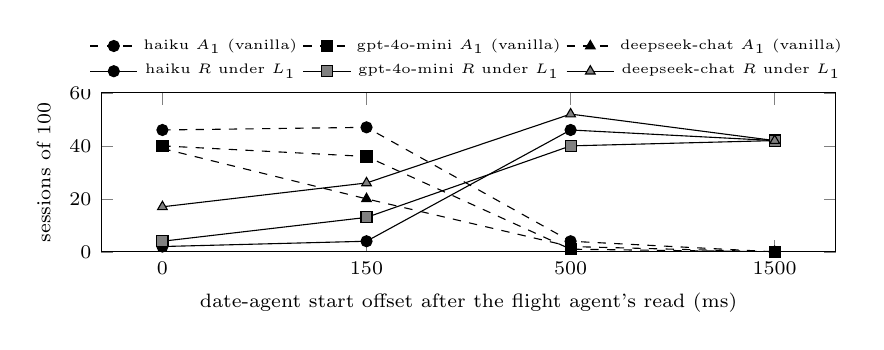
\begin{tikzpicture}
\begin{axis}[width=0.9\columnwidth, height=3.6cm, symbolic x coords={0,150,500,1500}, xtick=data,
  xlabel={date-agent start offset after the flight agent's read (ms)}, ylabel={sessions of 100}, ymin=0, ymax=60,
  legend style={font=\tiny, at={(0.5,1.02)}, anchor=south, legend columns=3, draw=none}, tick label style={font=\scriptsize}, label style={font=\scriptsize}, cycle list name=black white]
\addplot+[dashed, mark=*, mark options={solid}] coordinates {(0,46) (150,47) (500,4) (1500,0)};
\addlegendentry{haiku \A1 (vanilla)}
\addplot+[dashed, mark=square*, mark options={solid}] coordinates {(0,40) (150,36) (500,1) (1500,0)};
\addlegendentry{gpt-4o-mini \A1 (vanilla)}
\addplot+[dashed, mark=triangle*, mark options={solid}] coordinates {(0,39) (150,20) (500,2) (1500,0)};
\addlegendentry{deepseek-chat \A1 (vanilla)}
\addplot+[solid, mark=*] coordinates {(0,2) (150,4) (500,46) (1500,42)};
\addlegendentry{haiku \Rp{} under $L_1$}
\addplot+[solid, mark=square*] coordinates {(0,4) (150,13) (500,40) (1500,42)};
\addlegendentry{gpt-4o-mini \Rp{} under $L_1$}
\addplot+[solid, mark=triangle*] coordinates {(0,17) (150,26) (500,52) (1500,42)};
\addlegendentry{deepseek-chat \Rp{} under $L_1$}
\end{axis}
\end{tikzpicture}
\caption{Probe 303, offset sweep: the live \A1 rate without a discipline (dashed) and the residue \Rp{} that read-set validation leaves (solid) as the date agent's start is delayed; revision probability $0.5$, $n=100$ per point. As the window closes the same revisions land after the commit: \A1 falls to $0$ while \Rp{} rises to the revision rate.}
\label{fig:offset}
\end{figure}

\smallskip\noindent\textbf{What $L_1$ removes, and what it does not.}
Read-set validation removed every firing ($0/300$) at one discarded
generation per realized conflict (\LiveGptRegen{} and \LiveHaikuRegen{} per
$100$ sessions, never two in one session). It did not make the booking agree
with the final trip date: in $\LiveGptValidatedWrong$ and
$\LiveHaikuValidatedWrong$ of $100$ sessions the revision landed after the
commit---the committed record is current at its commit point exactly as
\cref{thm:corc} says, and the booking is stale with respect to a state that
did not yet exist. That residue is a post-commit supersession, the blind
overwrite of \cref{sec:a1}, serializable in commit order and outside every
isolation discipline; only compensation, or holding the effect until its
basis is final, reaches it. The \emph{sequential} control, clean under every
commit-time predicate, delivers the wrong booking in $100/100$ sessions for
the same reason; the predicate alone would have credited $L_1$ with a
correctness it does not provide.

\smallskip\noindent\textbf{\Rp{} decides the residue on the records.}
The \Rp{} column of \cref{tab:live} is decided on the emitted records alone:
the basis of each booking is the date value in its arguments, and \Rp{}
fires in exactly the sessions whose booking disagrees with the final date
and \A1 does not ($A_1+R=100$ in every unguarded cell; under $L_1$ the \Rp{}
column equals the residue; \texttt{a7\_rescore.py -{}-check}). The identity
is between two independent computations (\cref{sec:residue}) and holds
because the booking tool takes the date as a structured argument; a workload
whose effects paraphrase their inputs would show a coverage below
\HypBasisRecovered/\HypBookings{} and a smaller \Rp{} column, never a larger
one. Two further arms run on three API families (haiku, gpt-4o-mini and
deepseek-chat through its OpenAI-compatible endpoint). In the
\emph{verified} arm the $L_1$ decision is taken by the verified store through
the bridge of \cref{sec:trust}: \A1 fires in $0/300$ sessions and the
residue is $2$, $51$ and $52$ of $100$ against $12$, $51$ and $63$ for the
application-layer arm of the same run. In the \emph{ledger} arm a
superseding put registers the obligation and a compensator issues a
replacement booking: $0/100$ wrong on all three families ($5$, $45$ and $53$
obligations, each discharged by one compensation generation), at the price
of $L_1$'s discarded generations plus one per obligation.

\smallskip\noindent\textbf{What a difference between arms can mean, and
what the replication says.} The four arms of \cref{tab:live}'s October run
were sequential blocks of $100$ sessions, and the $L_1$ residue is the
share of revisions that landed after the commit---a race between two
provider latencies plus the fixed offset---so a latency drift between
blocks moves it without any change of discipline: the two $L_1$ arms on
haiku, one discipline decided in two places, differ at $12$ vs.\ $2$ of
$100$ (Fisher exact $p=\ArmFisherHaiku$). The attributable design
interleaves the arms per session in a seeded order and repeats the protocol
with fresh seeds; \cref{tab:liveruns} reports \LiveRunsHaiku{} such runs of
five arms per family (the fifth, \emph{ledger-verified}, is the ledger over
the verified store). Three things follow. The arms ran the same session
back to back, so the comparison is paired: the validated arm alone left the
residue in $\RunsPairedDiscordantHaiku$ sessions of $300$ on haiku (McNemar
exact $p\RunsMcNemarHaiku$; difference $\RunsDiffHaiku$ points, 95\%
$\RunsDiffCIHaiku$), $\RunsPairedDiscordantGpt$ on gpt-4o-mini
($p\RunsMcNemarGpt$; $\RunsDiffGpt$ $\RunsDiffCIGpt$) and
$\RunsPairedDiscordantDeepseek$ on deepseek-chat ($p\RunsMcNemarDeepseek$;
$\RunsDiffDeepseek$ $\RunsDiffCIDeepseek$): the replication detects no arm
difference and bounds one at a few points on haiku, about ten elsewhere;
the sequential-run haiku difference points the same way at a base rate
($2$ of $100$) that leaves no power. \A1 is $0$ in the $900$
October-sequential and $3{,}600$ interleaved sessions run under $L_1$ at
this offset. The run, not the arm, is where the residue moves: against the sequential
run, vanilla \A1 is $94$ vs.\ $\RunsHaikuVanillaAOnePooled$ on haiku
($p\RunsVsSeqHaikuVanillaAOne$) and $44$ vs.\ $\RunsGptVanillaAOnePooled$ on
gpt-4o-mini ($p\RunsVsSeqGptVanillaAOne$), the $L_1$ residue $12$ vs.\
$\RunsHaikuValidatedRPooled$ and $51$ vs.\ $\RunsGptValidatedRPooled$
($p\RunsVsSeqHaikuValidatedR$, $p\RunsVsSeqGptValidatedR$), and three
deepseek-chat runs of one arm span $54$--$73$; the split of the revision
rate into predicate and residue is the provider's latency at the hour of the
run, which a deployment reads off its own records, not off a table. And the
ledger rows do not move: $\RunsHaikuLedgerWrongPooled$ wrong bookings in
both ledger arms on every family (exact 95\% interval
$\RunsHaikuLedgerWrongCI$)---on the store, the qualification
\cref{sec:ledger-world} measures.

\ifnum\LiveRunsAvailable=1
\begin{table}[t]
\centering
\caption{Replicated, interleaved live study (probe 303 \texttt{-{}-interleave -{}-runs 3}): \Rp{} per run of $100$ sessions at the $150$\,ms offset, the five arms of a session run back to back in a seeded order, and the pooled count (exact 95\% intervals: supplement \S\,W). \A1 fired in $0/300$ sessions of every $L_1$ arm and in $\RunsHaikuVanillaAOnePooled$, $\RunsGptVanillaAOnePooled$ and $\RunsDeepseekVanillaAOnePooled$ vanilla sessions (per run \RunsHaikuVanillaAOneRuns, \RunsGptVanillaAOneRuns, \RunsDeepseekVanillaAOneRuns); booking $\neq$ final is $A_1+R$ in every cell. The ledger rows' \Rp{} is decided from the obligation record emitted at the superseding put; the share of revisions that landed after the final commit (wall-clock stamp) equals \Rp{} in the $L_1$ arms and the obligations registered in the ledger arms.}
\label{tab:liveruns}
\footnotesize
\setlength{\tabcolsep}{3pt}
\resizebox{\columnwidth}{!}{%
\begin{tabular}{@{}lccc@{}}
\toprule
Arm & haiku & gpt-4o-mini & deepseek-chat \\
\midrule
vanilla & \RunsHaikuVanillaRShort & \RunsGptVanillaRShort & \RunsDeepseekVanillaRShort \\
validated ($L_1$) & \RunsHaikuValidatedRShort & \RunsGptValidatedRShort & \RunsDeepseekValidatedRShort \\
verified ($L_1$, verified store) & \RunsHaikuVerifiedRShort & \RunsGptVerifiedRShort & \RunsDeepseekVerifiedRShort \\
ledger ($L_1{+}\ell$) & \RunsHaikuLedgerRShort & \RunsGptLedgerRShort & \RunsDeepseekLedgerRShort \\
ledger-verified & \RunsHaikuLedgerVerifiedRShort & \RunsGptLedgerVerifiedRShort & \RunsDeepseekLedgerVerifiedRShort \\
\bottomrule
\end{tabular}}
\end{table}
\fi

\smallskip\noindent\textbf{The offset sweep.} \Cref{fig:offset} varies the
race instead of fixing it: the date agent starts $0$, $150$, $500$ or
$1{,}500$\,ms after the flight agent's read and revises in about half the
sessions ($p=0.5$), $n=100$ per point on the three API families. Without a
discipline \A1 fires in $39$--$46$ of $100$ sessions at $0$\,ms and in $0$ at
$1{,}500$\,ms, where every revision lands after the commit, while the
booking is wrong in every revised session at every offset ($44$--$51$).
Under $L_1$ the curve inverts: the residue is $2$--$17$ at $0$\,ms and
$40$--$52$ at $500$--$1{,}500$\,ms, the discarded generations falling from
$34$--$49$ to $0$. Predicate and residue are the two halves of one quantity,
the revision rate, split by where the revision lands relative to the commit;
what the remark of \cref{sec:residue} says must remain after release does
remain under every commit-time discipline.

\smallskip\noindent\textbf{Superstep.} A second graph places a writer and a
summarizer of one reducer-declared channel in one Pregel
superstep~\cite{MalewiczEtAl2010Pregel}; the barrier hands both the snapshot
at superstep entry, so in $300/300$ sessions the summary names the
destination the writer had changed: the snapshot-insufficiency shape of
\cref{sec:snapshot} observed live, reported as documented BSP semantics, not
a rate (the census finds it in no public graph; under a completion clock
\cref{def:a1} fires in \SuperstepGpt, \SuperstepHaiku, \SuperstepLlama{} of
$100$).


\subsection{The ledger in a world: a consumer, a cancellation, a compensator that fails}
\label{sec:ledger-world}
The ledger arm's $0/300$ is a statement about the final store: the
compensator overwrote the booking cell, nothing read the first booking
before the compensation, the compensator could not fail, and the workload
revised once. None of that is true of a world, so we measure the same
discipline against one (probe 304): the booking is an
irreversible effect in an external service that stays active until
cancelled; a \emph{consumer}---a downstream reader that sends the
itinerary---reads the active bookings a uniform
$0$--$\LedgerWorldConsumerMaxMs$\,ms after the first release; the date agent
revises \emph{twice} ($150$\,ms and $+800$\,ms after the flight agent's
read); and the world refuses a
cancellation or a rebooking with probability $\LedgerWorldPCancelFail$ each,
in which case the obligation stays registered and open and is retried at the
next supersession. Three arms share every session's seed and run
interleaved: $L_1$ alone; $L_1$ with the ledger and a compensator that
cancels the stale booking and rebooks; and the same without the
cancellation, the compensator of \cref{tab:live} seen from the world.
Scored at the end of each session \emph{in the world}:
sessions with an active booking whose date is not the final date
(\emph{world wrong}), with two active bookings (\emph{double}), with none
(\emph{none}: the cancellation went through and the rebooking was refused),
and sessions whose consumer acted on a date that is not the final one
(\emph{consumer stale}) or found no booking (\emph{consumer none}).
\ifnum\LedgerWorldAvailable=1
\Cref{tab:ledgerworld} is the result on three families. Under $L_1$ alone
the second revision lands after the regenerated commit in
$\LWHaikuValidatedR$--$\LWGptValidatedR$ sessions, so \Rp{} fires, store and
world are wrong, and the consumer acted on a stale date in the same
sessions: with two revisions the residue of \cref{tab:live} is nearly total.
The ledger registers an obligation in every one of them and \Rp{} is $0$ in
all $300$ ledger sessions---and that is where its guarantee ends. At session
end the world holds a stale booking in
$\LWHaikuLedgerWorldWrong$--$\LWGptLedgerWorldWrong$ sessions per family (in
$\LWHaikuLedgerDouble$--$\LWGptLedgerDouble$ of them beside the new one: the
cancellation was refused) and no booking in
$\LWHaikuLedgerWorldNone$--$\LWDeepseekLedgerWorldNone$ (the rebooking was
refused), and the obligation behind each is open---counted, not hidden
(last column)---except in the sessions the next paragraph counts; those
shares are the injected refusal rate of $\LedgerWorldPCancelFail$ seen from
the other side (one to two obligations per session), not a finding about
the ledger. The
consumer, reading within $1.5$\,s of the first release,
acted on a stale booking in
$\LWHaikuLedgerConsumerStale$--$\LWDeepseekLedgerConsumerStale$ sessions and
found none in $\LWDeepseekLedgerConsumerNone$--$\LWHaikuLedgerConsumerNone$:
this compensator drafts the replacement by a model call \emph{between} the
cancellation and the rebooking and so opens a window of one model latency
in which the world holds nothing, a transient $L_1$ alone never produces;
the consumer saw the final booking in $1$--$5$ sessions of $100$. Without
the cancellation the world is wrong in $99$ and double-booked in
$\LWHaikuLedgerNoRollbackDouble$--$\LWDeepseekLedgerNoRollbackDouble$.

One number is the one no store can show. Among the ledger sessions whose
every obligation the ledger reports discharged
($\LWHaikuLedgerCleanSessions$, $\LWGptLedgerCleanSessions$ and
$\LWDeepseekLedgerCleanSessions$ of $100$), the world still holds a stale
booking in $\LWHaikuLedgerCleanWrong$, $\LWGptLedgerCleanWrong$ and
$\LWDeepseekLedgerCleanWrong$. The cause is in our compensator, not in the
ledger: it tracked one confirmation per effect, so a retry after a refused
cancellation cancelled the \emph{replacement}, left the original active and
reported success. The world check caught it. The probe's default compensator now tracks every confirmation the effect
created, cancels all of them on a retry and drafts the replacement before
touching the world; \cref{tab:ledgerworld} is the first run, reproducible
under \texttt{-{}-compensator latest}, and its rerun under the corrected
compensator is \Pending{runner step 18 rerun} and replaces these cells. The
lesson does not wait for it: \Rp{} and the ledger are bookkeeping about the
records, the world is the arbiter, and what a ledger buys in a world is its
compensator---a refusal made visible as an open obligation where the
compensator reports truthfully, and nothing where it does not.
\begin{table}[t]
\centering
\caption{The ledger in a world (probe 304, compensator \texttt{\LedgerWorldCompensator}), $n{=}100$ sessions per arm per family, two revisions per session, cancellation and rebooking each refused with probability $\LedgerWorldPCancelFail$/$\LedgerWorldPRebookFail$, consumer delay uniform $0$--$\LedgerWorldConsumerMaxMs$\,ms; arms interleaved per session. Columns: \Rp{} on the records; store $\neq$ final; world wrong / double / none at session end; consumer acted on a stale date / found none; obligations registered\,/\,discharged\,/\,left open.}
\label{tab:ledgerworld}
\footnotesize
\setlength{\tabcolsep}{3pt}
\resizebox{\columnwidth}{!}{%
\begin{tabular}{@{}llrrrrrrrr@{}}
\toprule
Model & Arm & \Rp{} & store & wrong & double & none & c.\,stale & c.\,none & obl. \\
\midrule
\multirow{3}{*}{haiku} & $L_1$ & \LWHaikuValidatedR & \LWHaikuValidatedStoreWrong & \LWHaikuValidatedWorldWrong & \LWHaikuValidatedDouble & \LWHaikuValidatedWorldNone & \LWHaikuValidatedConsumerStale & \LWHaikuValidatedConsumerNone & \LWHaikuValidatedObl \\
 & $L_1{+}\ell$, cancel & \LWHaikuLedgerR & \LWHaikuLedgerStoreWrong & \LWHaikuLedgerWorldWrong & \LWHaikuLedgerDouble & \LWHaikuLedgerWorldNone & \LWHaikuLedgerConsumerStale & \LWHaikuLedgerConsumerNone & \LWHaikuLedgerObl \\
 & $L_1{+}\ell$, no cancel & \LWHaikuLedgerNoRollbackR & \LWHaikuLedgerNoRollbackStoreWrong & \LWHaikuLedgerNoRollbackWorldWrong & \LWHaikuLedgerNoRollbackDouble & \LWHaikuLedgerNoRollbackWorldNone & \LWHaikuLedgerNoRollbackConsumerStale & \LWHaikuLedgerNoRollbackConsumerNone & \LWHaikuLedgerNoRollbackObl \\
\midrule
\multirow{3}{*}{gpt-4o-mini} & $L_1$ & \LWGptValidatedR & \LWGptValidatedStoreWrong & \LWGptValidatedWorldWrong & \LWGptValidatedDouble & \LWGptValidatedWorldNone & \LWGptValidatedConsumerStale & \LWGptValidatedConsumerNone & \LWGptValidatedObl \\
 & $L_1{+}\ell$, cancel & \LWGptLedgerR & \LWGptLedgerStoreWrong & \LWGptLedgerWorldWrong & \LWGptLedgerDouble & \LWGptLedgerWorldNone & \LWGptLedgerConsumerStale & \LWGptLedgerConsumerNone & \LWGptLedgerObl \\
 & $L_1{+}\ell$, no cancel & \LWGptLedgerNoRollbackR & \LWGptLedgerNoRollbackStoreWrong & \LWGptLedgerNoRollbackWorldWrong & \LWGptLedgerNoRollbackDouble & \LWGptLedgerNoRollbackWorldNone & \LWGptLedgerNoRollbackConsumerStale & \LWGptLedgerNoRollbackConsumerNone & \LWGptLedgerNoRollbackObl \\
\midrule
\multirow{3}{*}{deepseek-chat} & $L_1$ & \LWDeepseekValidatedR & \LWDeepseekValidatedStoreWrong & \LWDeepseekValidatedWorldWrong & \LWDeepseekValidatedDouble & \LWDeepseekValidatedWorldNone & \LWDeepseekValidatedConsumerStale & \LWDeepseekValidatedConsumerNone & \LWDeepseekValidatedObl \\
 & $L_1{+}\ell$, cancel & \LWDeepseekLedgerR & \LWDeepseekLedgerStoreWrong & \LWDeepseekLedgerWorldWrong & \LWDeepseekLedgerDouble & \LWDeepseekLedgerWorldNone & \LWDeepseekLedgerConsumerStale & \LWDeepseekLedgerConsumerNone & \LWDeepseekLedgerObl \\
 & $L_1{+}\ell$, no cancel & \LWDeepseekLedgerNoRollbackR & \LWDeepseekLedgerNoRollbackStoreWrong & \LWDeepseekLedgerNoRollbackWorldWrong & \LWDeepseekLedgerNoRollbackDouble & \LWDeepseekLedgerNoRollbackWorldNone & \LWDeepseekLedgerNoRollbackConsumerStale & \LWDeepseekLedgerNoRollbackConsumerNone & \LWDeepseekLedgerNoRollbackObl \\
\bottomrule
\end{tabular}}
\end{table}
\else
The run is \Pending{runner step 18, three families}; its table replaces this
sentence, and until then the ledger's $0/100$ must be read as the store-level
statement above and nothing more.
\fi

\subsection{RQ1 across three disciplines: the AutoGen pilot}
\label{sec:pilot}
An instrumentation layer exposes a two-phase \texttt{begin}/\texttt{commit}
API to LLM-driven agents under AutoGen~\cite{WuEtAl2023AutoGen}; the Rust
runtimes of \cref{sec:l1} sit behind it. Three workloads span the space from
concurrent to sequential: \emph{edit-review} (two agents both read
\texttt{doc} before either writes---overlap forced), \emph{plan-execute}
(strictly sequential---overlap forbidden) and \emph{triage} (a three-agent
pipeline whose overlap is left to the models); gpt-4o, $100$ sessions per
cell, three runtimes (run \texttt{\CostRun}; the table is in supplement
\S\,M). \A1 fires in $100\%$ / $0\%$ / $48\%$ of vanilla
sessions on the three workloads (triage replicated three times:
\PilotTriageRates; pooled \PilotTriagePooled), in $0\%$ everywhere under
pessimistic locking, and in $\PilotSiEditResidual\%$ / $0\%$ /
$\PilotSiTriageResidual\%$ under default snapshot isolation, whose residual
is its no-write bypass (a read-only commit is never validated: the
unfaithful emitter of Theorem L1j; SSI mode closes it). Both endpoints are
engineered, so this is a sensitivity check of the detector and the runtimes
on model-driven traces, not a prevalence; every edit-review witness is a
cold-start read, unlike the live study's supersessions. Pessimistic locking
reaches $0\%$ on edit-review by refusing the reviewer's operation in
$99/100$ sessions---the anomaly is absent because the work is---and on
triage by dropping one of three agents in $97/100$; the sessions that are
\emph{complete and clean} (no witness, every role that commits in the
unguarded cell also commits) are the number to read a prevention claim
against, and on triage they favor the unguarded baseline ($52$) over
default-SI ($45$) and locking ($3$); whether a dropped contribution or a
stale one is worse is the task's call, which is why \cref{sec:cost} prices
prevention per sound committed operation. A Claude Sonnet~4.5 rerun of the vanilla column with operation records reproduces the
two determinate cells (edit-review $100/100$, plan-execute $0/100$); its
triage cell was void, and the cause was the workload: the reporter's prompt
asked for ``a one-sentence bug description'' and supplied no bug, gpt-4o
invented one, and Sonnet wrote ``no bug description provided'' in $100/100$
sessions. The pilot now hands the reporter a concrete bug drawn by scenario
from a fixed list and records the protocol beside each cell; the Sonnet
triage cell rerun under it holds $100$ sessions of three or more events and
no void ticket. \ifnum\PilotClaudeAvailable=1 Scored by the verified
detector, the Sonnet cells fire \A1 in \VSClaudeEditReviewVanilla{} /
\VSClaudePlanExecuteVanilla{} / \VSClaudeTriageVanilla{} sessions
(vanilla), \VSClaudeEditReviewPess{} / \VSClaudePlanExecutePess{} /
\VSClaudeTriagePess{} (pessimistic) and \VSClaudeEditReviewSI{} /
\VSClaudePlanExecuteSI{} / \VSClaudeTriageSI{} (default-SI); a cell
printed as -- has not run.\else Its \A1 rate, like the Sonnet pessimistic
and snapshot-isolation cells, is to be scored by the verified detector of
step 14 and is \Pending{runner steps 11/14} (supplement \S\,M).\fi{} The
gpt-4o run predates the change and is reported as run.

\subsection{RQ1 for $L_2$: output commit on synthetic cascades and live verdicts}
\label{sec:l2-eval}
Three arms run the same $1{,}000$ seeded schedules at nominal chain depths
$2$, $3$ and $5$: a root commits, a chain of dependents reads the previous
cell and commits, one committed transaction is put under review and retracted
or approved, and in a quarter of scenarios the review arrives after that
transaction has released. The \emph{verified} arm is \texttt{l2\_exec.rs};
the \emph{unguarded} arm validates reads, releases at commit and flags only
the aborted transaction; the \emph{cascade} arm releases at commit and
cascades the abort. Each trace is scored under \cref{def:a3}, under the
surviving-dependent predicate, and by \emph{exposed effects}, effects out at
the end although the review asked to withdraw their basis, which reads no
flag (full table: supplement \S\,P). \Cref{def:a3} fires in
\LtwoDefThreeBaseline{} of $1{,}000$ schedules per depth under both
baselines and in none under the verified arm; the cascade arm satisfies its
own surviving-dependent predicate in every scenario while exposing exactly
as many effects as no discipline at all (\LtwoExposedBaseline{}), because it
flagged \LtwoRelabeled{} dependents \emph{after} their effects were out---a
cascade without output commit moves flags, not effects. The verified arm is
not zero on exposed effects: \LtwoExposedVerified{} effects in $199$
scenarios per depth, exactly those in which the review arrived after the
release and the retraction was refused. The figures decompose by arithmetic
($1{,}538 = 402 + 572 + 564$ at depth 2): the first term no runtime can
remove; the second any runtime that declines to release an operation under
review avoids; the third ($37$--$46\%$ of the unguarded exposure) is output
commit's own contribution, at a cost in delay, not liveness (every
committed, unaborted operation was eventually released). The quarter of
late reviews is a harness parameter, so the overall exposure reduction
($73$--$74\%$) is that parameter seen from the other side, not a finding.

\smallskip\noindent\textbf{Live verdicts.} A plan--execute--revise workload
driven by real models (a planner commits a plan; an executor reads it and
commits, acquiring the planner as predecessor; a supervisor decides whether
to retract) was recorded for $200$ sessions on each of three families and
replayed through the three arms. Retraction rates varied sharply---$1/200$
(claude-haiku-4-5), $3/200$ (gpt-4o-mini), $62/200$ (Llama-3.2)---so we
make the pooled statement only: in every one of
the \LiveLtwoRetractions{} retracted sessions the unguarded baseline and the
cascade design left a \cref{def:a3} witness (the latter while satisfying the
surviving-dependent predicate), and the verified runtime released no executor
effect on a retracted plan, at a pooled release rate of $89.0\%$. A further
$1{,}000$ haiku sessions produced no retraction at all, so on that family the
discipline's only observable cost is the hold: each kept effect waited for
the supervisor's verdict, a median $687$\,ms (p90 $789$\,ms). The zero is
structural; the \A3 hazard itself is a property of the backbone's
retraction rate, here $0/1{,}000$ to $62/200$.

\subsection{RQ1 for $L_3$: a released tool executor reorders}
\label{sec:a6-eval}
LangGraph's \texttt{ToolNode} dispatches a turn's tool calls concurrently
(\texttt{asyncio.gather}), collects results in input order and does not
serialize side effects; its tracker records a user needing sequential
execution for stateful tools and unable to obtain it (langgraphjs \#861). We
gave three backbones a natural prompt (no instruction to parallelize) over
five order-dependent infrastructure tools whose docstrings state their
dependencies, took the model-emitted call list as $\fld{io}$, and dispatched
it through the released \texttt{ToolNode} and through the $L_3$ sequencer.
Two things are real---whether a backbone batches an order-dependent
pipeline into one turn, and the executor---and per-tool latency is modeled,
drawn uniformly from $10$--$200$\,ms (a uniform-latency control produces no
reorder); the replay against real effects below removes the model.


The finding that survives the modeling is structural (table in
supplement \S\,P): gpt-4o-mini batches an order-dependent pipeline on
$\ToolNodeGptBatched/30$ turns, the full five-tool pipeline on
$\ToolNodeGptFull$ of them, and \texttt{ToolNode} commits
$\ToolNodeGptReordered$ of the $\ToolNodeGptBatched$ out of order ($0$ under
$L_3$); Llama-3.2 batches $\ToolNodeLlamaBatched/30$ and reorders
$\ToolNodeLlamaReordered$; claude-haiku-4-5 never batches ($0/30$); and the
transcript a developer inspects shows the correct order in all
\ToolNodeBatchedTurns{} batched turns while the external state does not in
\ToolNodeReorderings{} of them.
Calls emitted in one turn are, by the provider's contract, calls the model
declared parallelizable, so the defect is shared between a backbone that
misjudged independence and an executor that cannot notice; the $L_3$
sequencer makes effect order independent of the backbone, which the
cross-model spread shows cannot otherwise be assumed.
Replaying the $33$ recorded batches five times each through
\texttt{ToolNode} against real effects---a WAL-backed SQLite database and a
local HTTP service, with whatever latency those have---rather than a modeled
sleep, baseline \A6 fires in \ToolNodeRealSqlite{} replays (SQLite) and
\ToolNodeRealHttp{} (HTTP): the reorder is a property of concurrent dispatch
under any real latency, not of the distribution we drew. The $L_3$ arm of
that replay issued the calls one at a time, which cannot reorder and
measures nothing; \ifnum\ToolNodeVerifiedAvailable=1 the arm that counts
dispatches the batch concurrently through the same executor and releases
each real effect only when the verified sequencer (\cref{sec:l3}) releases
it: \A6 in \ToolNodeVerifiedSqlite{} replays (SQLite, baseline
\ToolNodeVerifiedBaselineSqlite{} in the same replays) and
\ToolNodeVerifiedHttp{} (HTTP, baseline \ToolNodeVerifiedBaselineHttp).\else
the arm that counts---concurrent dispatch through the same executor, each
real effect released only when the verified sequencer of \cref{sec:l3}
releases it---is \Pending{runner step 15}.\fi

\smallskip\noindent\textbf{$L_4$: validation at dispatch.}\label{sec:l4-eval}
One seeded schedule per run pins a tool and then revokes or re-signs random
tools; three dispatchers act on the same registry. Over $1{,}000$ runs at
registry widths $2$, $4$ and $16$ the churn touched the planned tool in
\LfourPhantom{} runs, and in exactly those runs both live resolution and
snapshot resolution called a phantom---Theorem $L_4$d measured rather than
argued---while the verified dispatcher (\texttt{l4\_exec.rs}, the verified
bytes) called none and refused exactly those runs; the informative figures
are the hazard rate and the refusal cost, the zero is Theorem $L_4$b
executing.

\subsection{RQ2: what prevention costs}
\label{sec:cost}
The pilot driver captures per-call usage and wall-clock for every session of
run \texttt{\CostRun} (gpt-4o, $900$ sessions) and of its Claude Sonnet~4.5
cost replication (September, without operation records: its guarded cells
price the disciplines without an \A1 verdict; \cref{sec:pilot}), at list
price at the time of the run. Per session,
snapshot isolation's token cost is not separable from the unguarded
runtime's on either provider (overlapping intervals in every cell), and
pessimistic locking's overhead is provider-dependent (at most $1.6\times$
on gpt-4o and $2.2\times$ on Claude, both on triage, where it retries). A
per-session denominator credits a discipline for work it declined to do, so
\cref{tab:cost} re-prices the same run per committed operation and per
\emph{sound} committed operation---one that is not the stale reader of any
\cref{def:a1} witness.

\begin{table}[t]
\centering
\caption{Token cost of prevention under three denominators, gpt-4o, run
\texttt{\CostRun}. Per sound committed operation is the price we recommend
reading. Underlying counts (commits / sound): edit-review vanilla $212/112$,
pessimistic $101/101$, SI $110/105$; triage vanilla $335/283$, pessimistic
$205/205$, SI $268/256$; plan-execute $\approx200/200$ for all three.}
\label{tab:cost}
\footnotesize
\setlength{\tabcolsep}{3.5pt}
\resizebox{\columnwidth}{!}{%
\begin{tabular}{@{}llrrr@{}}
\toprule
Workload & Discipline & per session & per commit & per sound commit \\
\midrule
edit-review  & pessimistic & $+3.8\%$  & $+117.9\%$ & $+15.1\%$ \\
edit-review  & SI          & $+0.6\%$  & $+94.0\%$  & $+7.4\%$  \\
plan-execute & pessimistic & $+1.7\%$  & $+1.2\%$   & $+1.2\%$  \\
plan-execute & SI          & $+0.4\%$  & $+0.4\%$   & $+0.4\%$  \\
triage       & pessimistic & $+42.7\%$ & $+133.2\%$ & $+97.0\%$ \\
triage       & SI          & $+0.5\%$  & $+25.6\%$  & $+11.1\%$ \\
\bottomrule
\end{tabular}}
\end{table}

Parity does not survive the change of denominator: snapshot isolation costs
$+7.4\%$, $+0.4\%$ and $+11.1\%$ per sound committed operation, and
pessimistic locking's triage penalty is $+97\%$ rather than $+43\%$.
Overhead tracks realized contention: edit-review, which aborts hardest, pays
most; plan-execute, which never aborts, pays at most $+1.7\%$ under any
denominator. A separate $155$-session paired sweep on gpt-4o-mini (fan-in
$2$--$16$ at one cell; $2$--$32$ cells at fan-in $8$; realized abort rates
$0.09$--$0.93$) resolves the mechanism: snapshot isolation carries no fixed
overhead (intercept $+0.05\%$, CI $[-1.5,+1.7]$) and pays $1.074\times$
$[1.052, 1.096]$ a first-attempt generation per abort, because the retry
carries the conflict into its prompt; the per-abort price does not steepen
with contention (supplement \S\,M).

\smallskip\noindent\textbf{Wall-clock, with its confound.} The nine cells of
a run were executed one after another, so a difference between cells carries
whatever the provider's latency did in between. Plan-execute, on which no
runtime aborts, is the control, and its ``overheads'' are $-4.5\%$ and
$-4.9\%$ on gpt-4o (Holm-corrected permutation $p=0.014$, $0.002$) and
$+13.5\%$ for SI on Claude ($p=0.001$): drift, whose largest magnitude we
report as the run's null band. Outside it, on mean and median alike:
pessimistic locking at $+16.7\%$ (edit-review) and $+34.9\%$ (triage) on
gpt-4o and $+109.5\%$ (triage) on Claude, where it makes $7.75$ model calls
per session against $4.00$. Snapshot isolation is inside the band in every
cell on both families, which is not zero: the design cannot resolve an
overhead below about $5\%$ on gpt-4o or $14\%$ on Claude, and the
per-sound-commit wall-clock overheads on gpt-4o, $+4.9\%$ $[-2.8, +13.5]$
and $+11.0\%$ $[-2.5, +26.1]$, have intervals that include both zero and the
band (every cell in supplement \S\,O). Only a rerun with the three runtimes
interleaved per session removes the confound; probe~302 is that design.
\ifnum\WallclockPairedClaudeAvailable=1 On Claude Sonnet~4.5 its paired
per-session overheads (mean, bootstrap 95\% CI) are triage pessimistic
\WallclockPairedClaudeTriagePess{} and SI \WallclockPairedClaudeTriageSI,
with the plan-execute control at \WallclockPairedClaudePlanExecutePess{} and
\WallclockPairedClaudePlanExecuteSI{} (supplement \S\,O for every
cell).\else Its Claude Sonnet~4.5 run is \Pending{runner step 6}; the
gpt-4o rerun is not planned, so the gpt-4o wall-clock cells above stand
with their null band and no finer claim is made for them.\fi

\subsection{RQ3: where the preconditions occur}
\label{sec:prevalence}
Every occurrence figure above is a race we opened or a rate on our own
workloads. To put a denominator under the structural precondition of \A1 in
the framework we studied---a reader and a writer of one last-value channel
released into the same superstep---we analyzed public code; the answer is a
bracket, \emph{none confirmed, at most about half}. \emph{Frame}: GitHub
repositories matching \texttt{langgraph} in name, description or readme
(Python; forks and the framework's own organization excluded), in three star
bands; $60$ drawn per band under a fixed seed from the API's $500$ most
recently updated. \emph{Instrument}: a static front end that recovers, from
the syntax tree alone, each \texttt{StateGraph} site, the node pairs one
fork releases into a superstep, and each node's read and written keys;
whatever it cannot resolve is \emph{unknown}, never guessed (eleven fixtures
pin its rules; a differential oracle agrees with execution on the eight
runnable ones). All $180$ repositories were read (per-band counts in
supplement \S\,Q); \CensusRepos{} contain a visible graph, holding
\CensusSites{} sites, of which \CensusSequential{} ($96\%$) are sequential.
Fifteen sites in \CensusParallelRepos{} repositories ($11.2\%$, Wilson 95\%
$[6.4, 19.0]$) contain a co-scheduled pair; none is a confirmed
reader/writer pair on a last-value channel (repository-level upper limit
$3.8\%$); two are such pairs on a reducer channel, the ordinary
parallel-agents-on-\texttt{messages} idiom; eight have an unresolved side,
bounding the susceptible share at $8.2\%$ $[4.2, 15.3]$ of repositories.
Counting every unresolved site ($82$ with unresolved routing, $7$ with a
\texttt{Send} fan-out) gives a wide bound of $51\%$. An enriched
population---the
\CensusErrorStringRepos{} third-party repositories whose issues quote
LangGraph's co-superstep writer/writer error, projects that demonstrably ran
parallel writers---has parallel graphs in $12/26$ but again no confirmed
site in $391$. The narrow reading is a negative result for the motivation
of \cref{sec:live-a1}, recorded as one; the census measures how code is
written, not how often a graph runs or whether a co-scheduled read goes
stale.

\smallskip\noindent\textbf{Mechanisms, not rates.} Of five deployed designs
we probed, four close the window by construction and LangGraph's superstep
channels and cross-thread store leave it open, which is where
\cref{sec:live-a1} measures it; the mechanisms, and two framework defects
outside the catalog (a sequential blind overwrite behind deer-flow \#3123;
\texttt{interrupt} emitting a pre-gate effect twice), are in supplement
\S\,Q.

\subsection{Threats to validity}
\label{sec:threats}
\emph{Construct.} \A1 tracks the window, not the harm; \cref{tab:live}
reports both and \Rp{} names the gap. The basis is argument provenance,
verbatim and not semantic. Whether a booking that disagrees with a later
revision is harm is the application's call; we count it because the user
asked for one trip. \A6 fires on commuting effects and is silent on dropped
ones. \emph{Internal.} The live rates are
latency races, $n=100$ per cell, single runs in \cref{tab:live} and
\cref{fig:offset} and three interleaved runs in \cref{tab:liveruns}; the
wall-clock cells carry a run-order confound we bound rather than remove
(probe~302 removes it; not run); the L2 live replay rests on $66$
retractions, $62$ from one family ($1{,}000$ further haiku sessions added
none). \emph{External.} Three API families and one local; one framework
driven live; toy workloads of two to three agents. \emph{Reproducibility.}
Every cell is committed with its traces and rescored by an independent
implementation of \cref{def:a1}; run \texttt{20260913T0424Z} carries a
manifest captured at run time, the two earlier runs carry reconstructed
manifests that say so.

% ============================================================================
% sec/07-related.tex
% ============================================================================
\section{Related work}
\label{sec:related}

\subsection{Classical consistency and isolation}
The hardware tradition~\cite{Lamport1979SC,HerlihyWing1990} characterizes
visibility under bounded latency; ours is unbounded. The database isolation
hierarchy~\cite{BerensonEtAl1995,Adya1999,AdyaLiskovOneil2000} is the direct
ancestor: we adopt its anomaly-based method over a different operational
model, and the SSI line~\cite{FeketeEtAl2005MakingSI,CahillRohmFekete2008SSI,PortsGrittner2012}
is the reference for our SSI runtime, the difference being that the work
discarded on abort is an inference. Weikum and Vossen's commit-order-preserving
serializability~\cite{WeikumVossen2001} and Kung and Robinson's backward
validation~\cite{KungRobinson1981OCC} are what \cref{thm:corc} mechanizes at
the level of values read; view equivalence~\cite{Papadimitriou1979} is where
the value-level and conflict-level notions meet. Highly available
transactions~\cite{BailisEtAl2014HAT} classify levels by admitted anomalies,
the method our lattice borrows; Cerone et al.~\cite{CeroneEtAl2015Framework}
give the axiomatic framework our predicates specialize;
\emph{robustness}~\cite{BernardiGotsman2016Robustness} is what the census
asks statically; our detectors are polynomial only because each predicate
is existential over a constant number of records. Compensation descends
from sagas~\cite{GarciaMolinaSalem1987Sagas}, its formal
treatment~\cite{KorthLevySilberschatz1990Compensating},
ConTracts~\cite{ReuterWachter1991ConTract} and Gray and
Reuter~\cite{GrayReuter1993}; recoverability and strictness are
Hadzilacos~\cite{Hadzilacos1988Reliability} and Bernstein et
al.~\cite{BernsteinHadzilacosGoodman1987}. Irrevocable
transactions~\cite{WelcEtAl2008Irrevocable} and transactional
boosting~\cite{HerlihyKoskinen2008Boosting} met the same irreversibility in
transactional memory; output commit is the dual choice. Commutativity-based
control~\cite{Weihl1988Commutativity} orders only what does not commute: an
\A6 discipline over commutativity classes would pay the sequencing cost only
where it buys something, since the premise of \A6 holds only for
non-commuting effects and our predicate over-reports on the rest. The basis
of \cref{def:residue} is why-provenance~\cite{BunemanEtAl2001Why} restricted
to copying; exactly-once stream processing~\cite{AkidauEtAl2013MillWheel}
holds side effects at a transactional sink until the input is durable, the
industrial precedent for output commit. The pessimistic/optimistic choice
our cost analysis turns on is STM's contention-management problem, and the
cost-aware selection of a level is consistency
rationing~\cite{KraskaEtAl2009Rationing} and
TxnSails~\cite{ZhouEtAl2025TxnSails}.

\subsection{Concurrency control and shared memory for LLM agents}
A 2025--2026 line builds mechanisms for this regime, mostly without verifying
them, and this paper is one point in it rather than its origin. Agentic
transactions~\cite{SunEtAl2026AgenticTx} recast ACID as four semantic
guarantees for a single long-horizon agent and measure task success, with no
history predicate, model or proof; our catalog is the anomaly-level account
such guarantees would be checked against (supplement \S\,D places it on the
lattice with the systems below). CoAgent~\cite{LyuEtAl2026CoAgent} states
the regime in our three terms and proposes an advisory protocol in which a
notified agent repairs its own plan; its correctness argument is conditional
on a model judgment measured at a $5\%$ failure rate, and its lock/OCC cost
inversion independently reproduces \cref{sec:cost}. STORM~\cite{LiuEtAl2026STORM} is read validation ($L_1$)
deployed per file; ATCC~\cite{ZhouEtAl2026ATCC} and GoEX~\cite{PatilEtAl2024GoEX}
impose a remedy from the runtime. MemTX~\cite{LiEtAl2026MemTX} is the closest
design to our $L_2$: staged writes under snapshot isolation, irreversible
tool calls gated on current belief and cascading repair on retraction, with
two invariants checked by bounded enumeration ($5.5$M states) and a
five-backbone evaluation; it does not state the predicates it excludes,
verify the runtime, or price prevention per unit of sound work. Yang et
al.~\cite{YangEtAl2026Position} argue that coordination failures attributed
to communication are concurrency failures; governed shared
memory~\cite{MargalitEtAl2026Governed} and transactive
memory~\cite{Transactive2026} address provenance, supersession and scoping
without treating the generation window as a transaction.
TOKI~\cite{Wang2026TOKI} is the closest formal treatment of supersession: it
casts contradiction resolution in agent memory as write-time concurrency
control, names the isolation each resolution operator presupposes and the
write anomalies it admits, and proves soundness of a bitemporal operator
family; it governs which belief a memory keeps, where \Rp{} governs what an
effect already out still owes, and the two are complementary.
SAFEFLOW~\cite{LiEtAl2025SAFEFLOW} combines transactional execution with
information-flow labels and write-ahead rollback at the coordination layer,
and Cordon~\cite{ChenEtAl2026Cordon} stages external actions in an effect
outbox released only after whole-workflow validation---output commit at
task granularity without a model of concurrent tasks or a proof.
StateFuse~\cite{VolkovEtAl2026StateFuse} keeps conflicting observations
visible under CRDT merging, a contract orthogonal to exclusion like
CodeCRDT's. Yu et al.~\cite{YuEtAl2026ExecConsistency} ask whether a
shared memory, however consistent, suffices for an agent's task duties, a
question above the history level at which we work.
SagaLLM~\cite{GengChang2025SagaLLM}, Atomix~\cite{MohammadiEtAl2026Atomix}
and CodeCRDT~\cite{Pugachev2025CodeCRDT} are placed on the lattice informally
in supplement \S\,D (none reaches $L_4$; \S\,V compares the nearest systems
dimension by dimension). S-Bus~\cite{Khan2026SBus} (the author's prior work)
recovers implicit read sets for one contract and is the natural supplier of
trust-base item (ix), with the limit stated there; agent-memory
systems~\cite{PackerEtAl2023MemGPT} and the
frameworks~\cite{LangGraph2026,WuEtAl2023AutoGen} supply substrate, not
contract.


\subsection{Commit-time guards, retraction, and what comes after commit}
\label{sec:related-residue}
The 2026 work on agent effects acts at the commit boundary:
CommitGuard~\cite{SantosGrueiro2026CommitGuard} licenses a durable effect
only by a witness still fresh at commit; Zheng et
al.~\cite{ZhengEtAl2026Stale} show that freshness guards of our $L_1$ kind
block $92$--$95\%$ of benign infrastructure races and argue for semantic
commit predicates; EffectMatch~\cite{ZhangEtAl2026EffectMatch} validates
persistent outcomes against what was approved; versioned
execution~\cite{ZhangEtAl2026Revisable} revokes an obsolete execution's
authority to publish. MemTX~\cite{LiEtAl2026MemTX} alone looks past
commit: on an explicit \emph{retraction} it walks a derivation DAG to
executed tool actions and records each as compensated or leaked. None
treats the ordinary case \cref{tab:live} measures---no retraction, no race,
a legitimate later write---or states what guarantee is achievable there;
the remark of \cref{sec:residue} says it is an obligation under an
open-world store, which the ledger registers atomically. The precision
objection of Zheng et al.\ is answered at the basis: a basis predicate
ignores writes to cells the effect never depended on.

\subsection{Effect order, durable execution, verified systems, taxonomies}
Parallel function calling is pursued deliberately
(LLMCompiler~\cite{KimEtAl2024LLMCompiler}, asynchronous
calling~\cite{GimEtAl2024AsyncLM}), with the ordering of
effects left to the runtime; \A6 is a wrong independence judgment seen at
the effect level (\cref{sec:a6-eval}). Sandboxes and policies for tool
effects~\cite{RuanEtAl2024ToolEmu,DebenedettiEtAl2024AgentDojo}
gate \emph{what} an agent may do, orthogonally to the order and basis of
effects; $\tau$-bench~\cite{YaoEtAl2024TauBench} scores end state for a
single agent. Durable-execution
engines~\cite{BurckhardtEtAl2021Durable} and exactly-once workflow
systems~\cite{SkiadopoulosEtAl2022DBOS}
govern whether an effect is \emph{repeated} after a crash---the property $D$
of \cref{sec:dup} names---while output commit governs whether it may
\emph{leave} while its basis can be withdrawn, and the two compose; rollback
recovery~
discharges duplicates by identity because replay is deterministic, a premise
agent runtimes break~\cite{ZhengEtAl2026ACRFence}. Retro~\cite{KimEtAl2010Retro} repair
effects that have already left by compensating requests; a refused
retraction in our $L_2$ is such an effect. IronFleet~\cite{HawblitzelEtAl2015IronFleet}
verify running protocols and stores, and Perennial~\cite{ChajedEtAl2019Perennial}
verify crash-safe storage by layered refinement, the template for the open
step of \cref{sec:l1}; ours are far smaller, and what they add is verified
bytes executed in a measurement. Jepsen~\cite{Kingsbury2013Jepsen} and the
black-box
checkers~\cite{TanEtAl2020Cobra,Aphyr2020Elle}
decide serializability over database histories with unverified analyzers
under a uniqueness assumption we share (\cref{sec:a3}); ours decide a far
simpler property and are verified against it, in the tradition of runtime
verification~\cite{BauerLeuckerSchallhart2011}.
MAST~\cite{CemriEtAl2025MAST} catalogs cognitive and coordination failures
and its traces cannot show \A1 either way (supplement \S\,C);
Agentproof~\cite{XavierEtAl2026Agentproof} analyzes agent graphs
statically, the programme the census specializes;
MCMAS~\cite{LomuscioQuRaimondi2017MCMAS} verifies task-level and strategic
properties, a complementary layer.

% ============================================================================
% sec/08-limitations.tex
% ============================================================================
\section{Limitations and future work}
\label{sec:limitations}

\noindent\emph{The predicates are coarser than the phenomena.} \A1
over-reports in one shape (a value overwritten and restored inside the
window; \HypRestored{} of \HypAOneWitnesses{} witness pairs on the live
records) and, as \cref{tab:live} shows, under-reaches the harm by the
post-commit supersession that \Rp{} names; \A6 fires on commuting effects
and is blind to dropped and duplicated ones. The detectors are sound and
complete against their Verus specifications, and \cref{tab:assurance} says
for each where specification and catalog definition coincide and under what
hypothesis.

\smallskip\noindent\emph{\Rp{} is not an anomaly, and its basis is
syntactic.} \Rp{} fires in $100/100$ sequential sessions because the
workload revises the date in every session; what \cref{tab:live}
establishes is that the harm an isolation discipline cannot reach is exactly
this predicate, not that concurrency causes it. Its basis is argument
provenance, a value that appears verbatim in an effect's arguments: a
booking derived from the date by computation (``the day after'') has an
empty basis and is invisible, so the extractor under-reaches and the \Rp{}
column is a lower bound; its coverage here is
\HypBasisRecovered/\HypBookings{} because the booking tool takes the date as
a structured argument, and free-text effects need a declared or
taint-tracked basis. The ledger's guarantee ends at registration; whether
an obligation is discharged, and at what cost, is the compensator's, and
\cref{sec:ledger-world} measures two of them on one workload.

\smallskip\noindent\emph{A refused retraction is not a prevented anomaly.}
Output commit makes \cref{def:a3} unreachable partly by holding effects and
partly by refusing to retract an operation whose effects are out; the second
leaves the world as it was and is counted (\cref{sec:l2-eval}); the
exposure--latency curve between the harness's one point and the live
driver's extreme is unmeasured.

\smallskip\noindent\emph{Verification is relative to the trace, and the
triangle closes on one system only in part.} Trust-base item (ix) is the
largest and is measured only at the store boundary: a value that reaches
the model through prompt context is invisible, and our own read-set
reconstruction finds most reads invisible on a realistic
workload~\cite{Khan2026SBus}. \ifnum\VerifiedScorerAvailable=1 The \A1
verdict is now the verified bytes behind an interning wrapper; the \A2,
\A3 and \A6 verdicts remain ports gated against their specifications.\else
The published \A1 verdicts stand on a gated port until the rescoring through
the verified bytes is committed; \A2, \A3 and \A6 remain ports gated against
their specifications.\fi{} The refinement from the two concurrent stores to
their abstract machines is open (a bounded simulation over $506{,}880$
transitions is evidence, not a proof); the $L_2$--$L_4$ exec artifacts are
sequential objects a multi-threaded caller must serialize; the ledger arm's
executable is harness code and the ledger's Verus model is scaffolding.
Liveness is verified nowhere.

\smallskip\noindent\emph{Prevalence is not established, and the census
points the other way.} The census bounds a structural precondition in public
code (none confirmed; at most about half counting every unresolved site)
and says nothing about private deployments, run frequency or the
cross-thread store variant; public LangGraph code rarely contends. Whether
these anomalies occur in production at a rate that justifies the costs of
\cref{sec:cost} is open; the live rates are latency races, and
\cref{tab:liveruns} shows them moving between runs of one arm by more than
between arms.

\smallskip\noindent\emph{Pending}, each a step of the artifact's runner and
each marked in the text where its receipt will land:
\ifnum\VerifiedScorerAvailable=0 the rescoring of every cell through the
verified detector (step 14; its first run rejected every record carrying
both \texttt{agent} and \texttt{agent\_id}, a reader defect fixed in this
version of the artifact, its rerun pending); \fi\ifnum\ToolNodeVerifiedAvailable=0 the
replay with the verified $L_3$ bytes (15); \fi\ifnum\LiveRunsAvailable=0
the replicated, interleaved live study with the ledger over the verified
store (17); \fi\ifnum\LedgerWorldAvailable=0 the ledger in a world (18);
\fi\ifnum\LedgerWorldFirstAvailable=0 the world study's rerun under the
corrected compensator (18); \fi\ifnum\WallclockPairedClaudeAvailable=0 the
interleaved cost rerun on Claude (6) and the Claude pilot's pessimistic and
snapshot-isolation cells, and the \A1 rate of its rerun triage cell (11,
14); \fi longer tasks, more agents and an instrumented deployment
remain the empirical follow-up; the store refinements, the formal one.

% ============================================================================
% sec/09-conclusion.tex
% ============================================================================
\section{Conclusion}
\label{sec:conclusion}

Four classical consistency conditions port to the regime in which an agent's
step spans an inference call, and the development is mechanized at stated
assurance levels: \TLA{} predicates with TLC witnesses, a realizability
matrix over every point of their exclusion lattice at stated bounds, a TLAPS
theorem placing stale-generation freedom as a conditional commit-order read
consistency, Verus detectors sound and complete against their specifications
with each specification's relation to its definition named, and four
disciplines verified in Verus and compiled byte-identical into the runtime,
\ifnum\ToolNodeVerifiedAvailable=1 all four\else three of them\fi{} executed
as the bytes that were verified. What the four leave is not an anomaly: an
effect out on a basis later writes revise, which under an open-world store
can only be owed, for which a basis ledger registers the obligation
atomically at every lattice point and, with a compensator, removes the
residue on the store---while in a world the ledger is worth exactly what
its compensator does, and the world check caught our own compensator
misreporting. The evaluation's contribution is not the verified arms'
zeros, which are theorems, but what sits beside them: the harm each
discipline leaves (\Rp{} in $1$--$65\%$ of live sessions per family and arm
under $L_1$ at $150$\,ms and up to $52\%$ as the race offset grows; $402$--$549$ exposed
effects per $1{,}000$ cascades under $L_2$), its cost per unit of sound work
($+0.4$--$11\%$ for snapshot isolation, up to $+97\%$ for locking), where
the preconditions occur in deployed code (nowhere confirmed in $407$ public
LangGraph sites for \A1; $30/30$ turns of one backbone's tool batching for
\A6; a resumption path that emits an effect twice), and which comparisons
its own design cannot support; the artifact re-derives each from committed
data.


% ============================================================================
% bib.tex
% ============================================================================
\begin{thebibliography}{100}
\bibitem{GengChang2025SagaLLM}
E.~Y. Chang and L.~Geng, ``{SagaLLM}: Context management, validation, and
  transaction guarantees for multi-agent {LLM} planning,'' \emph{Proceedings of
  the VLDB Endowment}, 2025, arXiv:2503.11951.

\bibitem{MohammadiEtAl2026Atomix}
B.~Mohammadi, N.~Potamitis, L.~Klein, A.~Arora, and L.~Bindschaedler, ``Atomix:
  Timely, transactional tool use for reliable agentic workflows,'' \emph{arXiv
  preprint arXiv:2602.14849}, 2026, preprint; not yet peer-reviewed at time of
  writing.

\bibitem{WeikumVossen2001}
G.~Weikum and G.~Vossen, \emph{Transactional Information Systems: Theory,
  Algorithms, and the Practice of Concurrency Control and Recovery}.\hskip 1em
  plus 0.5em minus 0.4em\relax Morgan Kaufmann, 2001.

\bibitem{KungRobinson1981OCC}
H.~T. Kung and J.~T. Robinson, ``On optimistic methods for concurrency
  control,'' \emph{ACM Transactions on Database Systems}, vol.~6, no.~2,
  pp. 213--226, 1981.

\bibitem{Lamport1979SC}
L.~Lamport, ``How to make a multiprocessor computer that correctly executes
  multiprocess programs,'' \emph{IEEE Transactions on Computers}, vol. C-28,
  no.~9, pp. 690--691, 1979.

\bibitem{HerlihyWing1990}
M.~P. Herlihy and J.~M. Wing, ``Linearizability: A correctness condition for
  concurrent objects,'' \emph{ACM TOPLAS}, vol.~12, no.~3, pp. 463--492, 1990.

\bibitem{BerensonEtAl1995}
H.~Berenson, P.~Bernstein, J.~Gray, J.~Melton, E.~O'Neil, and P.~O'Neil, ``A
  critique of {ANSI} {SQL} isolation levels,'' in \emph{ACM SIGMOD}, 1995, pp.
  1--10.

\bibitem{Adya1999}
A.~Adya, ``Weak consistency: A generalized theory and optimistic
  implementations for distributed transactions,'' Ph.D. dissertation, MIT,
  1999.

\bibitem{AdyaLiskovOneil2000}
A.~Adya, B.~Liskov, and P.~O'Neil, ``Generalized isolation level definitions,''
  in \emph{Proceedings of the 16th International Conference on Data Engineering
  ({ICDE})}, 2000, pp. 67--78.

\bibitem{LloydEtAl2011COPS}
W.~Lloyd, M.~J. Freedman, M.~Kaminsky, and D.~G. Andersen, ``Don't settle for
  eventual: Scalable causal consistency for wide-area storage with {COPS},'' in
  \emph{SOSP}, 2011, pp. 401--416.

\bibitem{CemriEtAl2025MAST}
M.~Cemri, M.~Z. Pan, S.~Yang, L.~A. Agrawal, B.~Chopra, R.~Tiwari, K.~Keutzer,
  A.~Parameswaran, D.~Klein, K.~Ramchandran, M.~Zaharia, J.~E. Gonzalez, and
  I.~Stoica, ``Why do multi-agent {LLM} systems fail?'' in \emph{NeurIPS
  Datasets and Benchmarks Track}, 2025, spotlight; arXiv:2503.13657.

\bibitem{CahillRohmFekete2008SSI}
M.~J. Cahill, U.~R{\"o}hm, and A.~D. Fekete, ``Serializable isolation for
  snapshot databases,'' in \emph{Proceedings of the {ACM} {SIGMOD}
  International Conference on Management of Data}, 2008, pp. 729--738.

\bibitem{Lamport1978TimeClocks}
L.~Lamport, ``Time, clocks, and the ordering of events in a distributed
  system,'' \emph{Communications of the ACM}, vol.~21, no.~7, pp. 558--565,
  1978.

\bibitem{WuEtAl2023AutoGen}
Q.~Wu, G.~Bansal, J.~Zhang, Y.~Wu, S.~Zhang, E.~Zhu, B.~Li, L.~Jiang, X.~Zhang,
  and C.~Wang, ``{AutoGen}: Enabling next-gen {LLM} applications via
  multi-agent conversation,'' in \emph{arXiv preprint arXiv:2308.08155}, 2023.

\bibitem{Miller2006Robust}
M.~S. Miller, ``Robust composition: Towards a unified approach to access
  control and concurrency control,'' Ph.D. dissertation, Johns Hopkins
  University, 2006.

\bibitem{BernsteinHadzilacosGoodman1987}
P.~A. Bernstein, V.~Hadzilacos, and N.~Goodman, \emph{Concurrency Control and
  Recovery in Database Systems}.\hskip 1em plus 0.5em minus 0.4em\relax
  Addison-Wesley, 1987.

\bibitem{GarciaMolinaSalem1987Sagas}
H.~Garcia-Molina and K.~Salem, ``Sagas,'' in \emph{Proceedings of the 1987 ACM
  SIGMOD International Conference on Management of Data}, 1987, pp. 249--259.

\bibitem{StromYemini1985OptimisticRecovery}
R.~E. Strom and S.~Yemini, ``Optimistic recovery in distributed systems,''
  \emph{ACM Transactions on Computer Systems}, vol.~3, no.~3, pp. 204--226,
  1985.

\bibitem{KorthLevySilberschatz1990Compensating}
H.~F. Korth, E.~Levy, and A.~Silberschatz, ``A formal approach to recovery by
  compensating transactions,'' in \emph{Proceedings of the 16th International
  Conference on Very Large Data Bases (VLDB)}, 1990, pp. 95--106.

\bibitem{FeketeEtAl2005MakingSI}
A.~Fekete, D.~Liarokapis, E.~O'Neil, P.~O'Neil, and D.~Shasha, ``Making
  snapshot isolation serializable,'' \emph{ACM Transactions on Database Systems
  ({TODS})}, vol.~30, no.~2, pp. 492--528, 2005.

\bibitem{Lattuada2023Verus}
A.~Lattuada, T.~Hance, C.~Cho, M.~Brun, I.~Subasinghe, Y.~Zhou, J.~Howell,
  B.~Parno, and C.~Hawblitzel, ``Verus: Verifying {Rust} programs using linear
  ghost types,'' in \emph{Proceedings of the {ACM} on Programming Languages
  (OOPSLA)}, vol.~7, 2023, pp. 286--315.

\bibitem{AnthropicMCP2024}
{Anthropic}, ``Model context protocol,'' \url{https://modelcontextprotocol.io},
  2024.

\bibitem{MalewiczEtAl2010Pregel}
G.~Malewicz, M.~H. Austern, A.~J.~C. Bik, J.~C. Dehnert, I.~Horn,
  N.~Leiser, and G.~Czajkowski, ``Pregel: A system for large-scale graph
  processing,'' in \emph{Proceedings of the ACM SIGMOD International
  Conference on Management of Data}, 2010, pp. 135--146.

\bibitem{Pugachev2025CodeCRDT}
S.~Pugachev, ``{CodeCRDT}: Observation-driven coordination for multi-agent
  {LLM} code generation,'' \emph{arXiv preprint arXiv:2510.18893}, 2025.

\bibitem{PortsGrittner2012}
D.~R.~K. Ports and K.~Grittner, ``Serializable snapshot isolation in
  {PostgreSQL},'' \emph{Proceedings of the VLDB Endowment}, vol.~5, no.~12,
  pp. 1850--1861, 2012.

\bibitem{Papadimitriou1979}
C.~H. Papadimitriou, ``The serializability of concurrent database updates,''
  \emph{J. ACM}, vol.~26, no.~4, pp. 631--653, 1979.

\bibitem{CeroneEtAl2015Framework}
A.~Cerone, G.~Bernardi, and A.~Gotsman, ``A framework for transactional
  consistency models with atomic visibility,'' in \emph{26th International
  Conference on Concurrency Theory (CONCUR)}, ser. LIPIcs, vol.~42, 2015,
  pp. 58--71.

\bibitem{BernardiGotsman2016Robustness}
G.~Bernardi and A.~Gotsman, ``Robustness against consistency models with
  atomic visibility,'' in \emph{27th International Conference on Concurrency
  Theory (CONCUR)}, ser. LIPIcs, vol.~59, 2016, pp. 7:1--7:15.

\bibitem{WelcEtAl2008Irrevocable}
A.~Welc, B.~Saha, and A.-R. Adl-Tabatabai, ``Irrevocable transactions and
  their applications,'' in \emph{Proc. 20th ACM Symp. Parallelism in Algorithms
  and Architectures (SPAA)}, 2008.

\bibitem{HawblitzelEtAl2015IronFleet}
C.~Hawblitzel, J.~Howell, M.~Kapritsos, J.~R. Lorch, B.~Parno, M.~L. Roberts,
  S.~Setty, and B.~Zill, ``{IronFleet}: Proving practical distributed systems
  correct,'' in \emph{Proceedings of the 25th ACM Symposium on Operating
  Systems Principles (SOSP)}, 2015, pp. 1--17.

\bibitem{Kingsbury2013Jepsen}
K.~Kingsbury, ``Jepsen: Distributed systems safety analysis,''
  \url{https://jepsen.io}, 2013--present, accessed 2026.

\bibitem{TanEtAl2020Cobra}
C.~Tan, C.~Zhao, S.~Mu, and M.~Walfish, ``{Cobra}: Making transactional
  key-value stores verifiably serializable,'' in \emph{Proceedings of the 14th
  {USENIX} Symposium on Operating Systems Design and Implementation ({OSDI})},
  2020, pp. 63--80.

\bibitem{Aphyr2020Elle}
K.~Kingsbury and P.~Alvaro, ``{Elle}: Inferring isolation anomalies from
  experimental observations,'' arXiv:2003.10554, 2020.

\bibitem{KimEtAl2024LLMCompiler}
S.~Kim, S.~Moon, R.~Tabrizi, N.~Lee, M.~W. Mahoney, K.~Keutzer, and
  A.~Gholami, ``An {LLM} compiler for parallel function calling,'' in
  \emph{Proc. 41st Int. Conf. Machine Learning (ICML)}, 2024.

\bibitem{YaoEtAl2024TauBench}
S.~Yao, N.~Shinn, P.~Razavi, and K.~Narasimhan, ``$\tau$-bench: A benchmark for
  tool-agent-user interaction in real-world domains,'' arXiv:2406.12045, 2024.

\bibitem{DebenedettiEtAl2024AgentDojo}
E.~Debenedetti, J.~Zhang, M.~Balunovi\'c, L.~Beurer-Kellner, M.~Fischer, and
  F.~Tram\`er, ``{AgentDojo}: A dynamic environment to evaluate prompt
  injection attacks and defenses for {LLM} agents,'' in \emph{Advances in
  Neural Information Processing Systems (NeurIPS), Datasets and Benchmarks
  Track}, 2024.

\bibitem{BurckhardtEtAl2021Durable}
S.~Burckhardt, C.~Gillum, D.~Justo, K.~Kallas, C.~McMahon, and C.~S.
  Meiklejohn, ``Durable Functions: Semantics for stateful serverless,''
  \emph{Proceedings of the ACM on Programming Languages (OOPSLA)},
  vol.~5, 2021.

\bibitem{LyuEtAl2026CoAgent}
H.~Lyu, D.~Zhang, M.~Wu, X.~Wei, and H.~Chen, ``{CoAgent}: Concurrency control
  for multi-agent systems,'' arXiv preprint arXiv:2606.15376, 2026.

\bibitem{LiuEtAl2026STORM}
M.~Liu, T.~Chen, Z.~Xu, X.~Jiang, and Y.~Dong, ``Multi-agent collaboration with
  state management,'' arXiv preprint arXiv:2605.20563, 2026.

\bibitem{Khan2026SBus}
S.~Khan, ``{S-Bus}: Automatic read-set reconstruction for multi-agent {LLM}
  state coordination,'' arXiv preprint arXiv:2605.17076, 2026.

\bibitem{ZhouEtAl2026ATCC}
W.~Zhou, Z.~Wang, Z.~Peng, H.~Chen, Y.~Zhang, and G.~Yu, ``{ATCC}: Adaptive
  concurrency control for unforeseen agentic transactions,'' arXiv preprint
  arXiv:2603.13906, 2026.

\bibitem{PatilEtAl2024GoEX}
S.~G. Patil, T.~Zhang, V.~Fang, Noppapon~C., R.~Huang, A.~Hao, M.~Casado,
  J.~E. Gonzalez, R.~A. Popa, and I.~Stoica, ``{GoEX}: Perspectives and designs
  towards a runtime for autonomous {LLM} applications,'' arXiv preprint
  arXiv:2404.06921, 2024.

\bibitem{XavierEtAl2026Agentproof}
M.~Xavier, Vaisakh~M.~A., M.~Jolly, and M.~Xavier, ``{Agentproof}: Static
  verification of agent workflow graphs,'' arXiv preprint arXiv:2603.20356,
  2026.

\bibitem{Hadzilacos1988Reliability}
V.~Hadzilacos, ``A theory of reliability in database systems,'' \emph{J. ACM},
  vol.~35, no.~1, pp. 121--145, 1988.

\bibitem{KimEtAl2010Retro}
T.~Kim, X.~Wang, N.~Zeldovich, and M.~F. Kaashoek, ``Intrusion recovery using
  selective re-execution,'' in \emph{Proc. 9th USENIX Symp. Operating Systems
  Design and Implementation (OSDI)}, 2010.

\bibitem{SkiadopoulosEtAl2022DBOS}
A.~Skiadopoulos, Q.~Li, P.~Kraft, K.~Kaffes, D.~Hong, S.~Mathew, D.~Bestor,
  M.~Cafarella, V.~Gadepally, G.~Graefe, J.~Kepner, C.~Kozyrakis, T.~Kraska,
  M.~Stonebraker, L.~Suresh, and M.~Zaharia, ``{DBOS}: A {DBMS}-oriented
  operating system,'' \emph{Proceedings of the VLDB Endowment}, vol.~15,
  no.~1, pp. 21--30, 2021.

\bibitem{PackerEtAl2023MemGPT}
C.~Packer, V.~Fang, S.~G. Patil, K.~Lin, S.~Wooders, and J.~E. Gonzalez,
  ``{MemGPT}: Towards {LLMs} as operating systems,'' \emph{arXiv preprint
  arXiv:2310.08560}, 2023.

\bibitem{ReuterWachter1991ConTract}
A.~Reuter and H.~W{\"a}chter, ``The {ConTract} model,'' \emph{IEEE Data
  Engineering Bulletin}, vol.~14, no.~1, pp. 39--43, 1991.

\bibitem{ChajedEtAl2019Perennial}
T.~Chajed, J.~Tassarotti, M.~F. Kaashoek, and N.~Zeldovich, ``Verifying
  concurrent, crash-safe systems with {Perennial},'' in \emph{Proc. 27th ACM
  Symposium on Operating Systems Principles (SOSP)}, 2019, pp. 243--258.

\bibitem{BauerLeuckerSchallhart2011}
A.~Bauer, M.~Leucker, and C.~Schallhart, ``Runtime verification for {LTL} and
  {TLTL},'' \emph{ACM Transactions on Software Engineering and Methodology},
  vol.~20, no.~4, pp. 14:1--14:64, 2011.

\bibitem{LomuscioQuRaimondi2017MCMAS}
A.~Lomuscio, H.~Qu, and F.~Raimondi, ``{MCMAS}: an open-source model checker
  for the verification of multi-agent systems,'' \emph{International Journal
  on Software Tools for Technology Transfer}, vol.~19, no.~1, pp. 9--30, 2017.

\bibitem{ZhengEtAl2026ACRFence}
Y.~Zheng, Y.~Yang, W.~Zhang, and A.~Quinn, ``{ACRFence}: Preventing semantic
  rollback attacks in agent checkpoint-restore,'' arXiv preprint
  arXiv:2603.20625, 2026.

\bibitem{ZhouEtAl2025TxnSails}
W.~Zhou, Y.~Zhang, Z.~Peng, and G.~Yu, ``{TxnSails}: Achieving serializable
  transaction scheduling with self-adaptive isolation level selection,'' arXiv
  preprint arXiv:2502.00991, 2025.

\bibitem{GrayReuter1993}
J.~Gray and A.~Reuter, \emph{Transaction Processing: Concepts and Techniques}.\hskip 1em plus 0.5em minus 0.4em\relax Morgan Kaufmann, 1993.

\bibitem{HerlihyKoskinen2008Boosting}
M.~Herlihy and E.~Koskinen, ``Transactional boosting: A methodology for highly-concurrent transactional objects,'' in \emph{Proc. 13th ACM SIGPLAN Symp. Principles and Practice of Parallel Programming (PPoPP)}, 2008, pp. 207--216.

\bibitem{KraskaEtAl2009Rationing}
T.~Kraska, M.~Hentschel, G.~Alonso, and D.~Kossmann, ``Consistency rationing in the cloud: Pay only when it matters,'' \emph{Proceedings of the VLDB Endowment}, vol.~2, no.~1, pp. 253--264, 2009.

\bibitem{LiEtAl2026MemTX}
X.~Li, Y.~Wang, H.~Lu, Z.~Chen, M.~Li, P.~Song, M.~Zheng, and T.~Cai, ``{MemTX}: Transactional belief commit for stateful agent memory,'' arXiv preprint arXiv:2607.23929, 2026.

\bibitem{YangEtAl2026Position}
X.~Yang, L.~Li, Z.~Ji, T.~J. Zhang, and W.~Jiang, ``Position: Multi-agent systems should prioritize concurrency control,'' arXiv preprint arXiv:2608.18092, 2026.

\bibitem{MargalitEtAl2026Governed}
Y.~Margalit, N.~Cohen-Inger, E.~Avram, R.~Taig, and O.~Margalit, ``Governed shared memory for multi-agent {LLM} systems,'' arXiv preprint arXiv:2606.24535, 2026.

\bibitem{Transactive2026}
T.~E. Kim, X.~He, D.~Jain, A.~Agrawal, N.~Arabzadeh, and F.~Diaz, ``Multi-agent transactive memory,'' arXiv preprint arXiv:2606.19911, 2026.

\bibitem{GimEtAl2024AsyncLM}
I.~Gim, S.~Lee, and L.~Zhong, ``Asynchronous {LLM} function calling,'' arXiv preprint arXiv:2412.07017, 2024.

\bibitem{RuanEtAl2024ToolEmu}
Y.~Ruan, H.~Dong, A.~Wang, S.~Pitis, Y.~Zhou, J.~Ba, Y.~Dubois, C.~J. Maddison, and T.~Hashimoto, ``Identifying the risks of {LM} agents with an {LM}-emulated sandbox,'' in \emph{Int. Conf. Learning Representations (ICLR)}, 2024.

\bibitem{SantosGrueiro2026CommitGuard}
I.~Santos-Grueiro, ``Temporary authority, permanent effects: Commit-time authorization for {LLM} agents,'' arXiv preprint arXiv:2607.10487, 2026.

\bibitem{ZhengEtAl2026Stale}
Z.~Zheng, J.~Long, B.~Li, and J.~Yao, ``Stale does not mean unsafe: Guard precision for tool-using {LLM} agents under infrastructure state races,'' arXiv preprint arXiv:2609.29522, 2026.

\bibitem{ZhangEtAl2026EffectMatch}
H.~Zhang, H.~Zhang, Z.~Liang, Y.~Yan, D.~Zuo, and H.~Wang, ``Beyond approved actions: Runtime validation of persistent outcomes in agent workflows,'' arXiv preprint arXiv:2609.31301, 2026.

\bibitem{ZhangEtAl2026Revisable}
Y.~Zhang, R.~Sharma, N.~Vegesna, Z.~Fu, C.~Liu, and T.~Krishnamurthy, ``Serving a revisable world: Versioned execution for interruptible agents,'' arXiv preprint arXiv:2610.01160, 2026.

\bibitem{BailisEtAl2014HAT}
P.~Bailis, A.~Davidson, A.~Fekete, A.~Ghodsi, J.~M. Hellerstein, and I.~Stoica, ``Highly available transactions: Virtues and limitations,'' \emph{Proc. VLDB Endow.}, vol.~7, no.~3, pp. 181--192, 2014.

\bibitem{Weihl1988Commutativity}
W.~E. Weihl, ``Commutativity-based concurrency control for abstract data types,'' \emph{IEEE Trans. Comput.}, vol.~37, no.~12, pp. 1488--1505, 1988.

\bibitem{BunemanEtAl2001Why}
P.~Buneman, S.~Khanna, and W.-C. Tan, ``Why and where: A characterization of data provenance,'' in \emph{Proc. ICDT}, 2001, pp. 316--330.

\bibitem{GuptaMumick1995ViewMaint}
A.~Gupta and I.~S. Mumick, ``Maintenance of materialized views: Problems, techniques, and applications,'' \emph{IEEE Data Eng. Bull.}, vol.~18, no.~2, pp. 3--18, 1995.

\bibitem{AkidauEtAl2013MillWheel}
T.~Akidau, A.~Balikov, K.~Bekiro\u{g}lu, S.~Chernyak, J.~Haberman, R.~Lax, S.~McVeety, D.~Mills, P.~Nordstrom, and S.~Whittle, ``{MillWheel}: Fault-tolerant stream processing at internet scale,'' \emph{Proc. VLDB Endow.}, vol.~6, no.~11, pp. 1033--1044, 2013.

\bibitem{SunEtAl2026AgenticTx}
Z.~Sun, X.~Wang, and G.~Li, ``Agentic transaction: Towards {ACID}-compliant agent systems,'' arXiv preprint arXiv:2608.13900, 2026.

\bibitem{LangGraph2026}
{LangGraph} 1.2, {Letta}, {CrewAI} 1.15, GitHub repositories, 2026.

\bibitem{Wang2026TOKI}
Z.~Wang, ``{TOKI}: A bitemporal operator algebra for contradiction resolution
  in {LLM}-agent persistent memory,'' \emph{arXiv preprint arXiv:2606.06240},
  2026.

\bibitem{LiEtAl2025SAFEFLOW}
P.~Li, Z.~Wu, Y.~Zhang \emph{et~al.}, ``{SAFEFLOW}: A principled protocol for
  trustworthy and transactional autonomous agent systems,'' \emph{arXiv
  preprint arXiv:2506.07564}, 2025.

\bibitem{ChenEtAl2026Cordon}
Z.~Chen, H.~Liu, D.~Xu, D.~Dong, J.~Li, B.~Pu, and J.~Zhai, ``Cordon: Semantic
  transactions for tool-using {LLM} agents,'' \emph{arXiv preprint
  arXiv:2606.17573}, 2026.

\bibitem{VolkovEtAl2026StateFuse}
S.~Volkov, Y.~Li, and Y.~Luo, ``{StateFuse}: Deterministic conflict-preserving
  memory for multi-agent systems,'' \emph{arXiv preprint arXiv:2607.05844},
  2026.

\bibitem{YuEtAl2026ExecConsistency}
Z.~Yu, Z.~Wang, P.~Wang, H.~Lin, R.~Zhao, and C.~Qin, ``Beyond corrected
  memory: Execution consistency in multi-agent systems,'' \emph{arXiv preprint
  arXiv:2610.08101}, 2026.

\end{thebibliography}


\end{document}
